
% ------------------ DOCUMENT SETUP ------------------ 
% The document class defines the document type (report) and sets the font size (12pt)
\documentclass[12pt]{report}
\author{Yie Nian Chu}


% Inputs the Document Packages
% ------------------ PACKAGES ------------------ 
% Packages add extra commands and features to your LaTeX document. 
% In here, some of the most common packages for a thesis document have been added 

% LaTeX's float package
\usepackage{float}

% LaTeX's color package
\usepackage{color}

% LaTeX's main math package
\usepackage{amsmath}

% LaTeX's Caption and subcaption packages
\usepackage[format=plain,font=footnotesize,labelfont=bf]{caption}
\usepackage{subcaption}

% The graphicx package provides graphics support for adding pictures.
\usepackage{graphicx}

% Longtable allows you to write tables that continue to the next page.
\usepackage{longtable}

% The geometry packages defines the page layout (page dimensions, margins, etc)
\usepackage[a4paper, lmargin=2.5cm, rmargin=2.5cm, tmargin=2.5cm, bmargin=2.5cm]{geometry}

% Defines the Font of the document, e.g. Arimo font (Check Fonts here: https://tug.org/FontCatalogue/)
\usepackage[sfdefault]{arimo}

% Font encoding
\usepackage[T1]{fontenc}

% This package allows the user to specify the input encoding
\usepackage[utf8]{inputenc}

% This package allows you to add empty pages
\usepackage{emptypage}

% Allows inputs to be imported from a directory
\usepackage{import}

% Provides control over the typography of the Table of Contents, List of Figures and List of Tables
\usepackage{tocloft}

% The setspace package controls the line spacing properties.
\usepackage{setspace}

% Allows the customization of Latex's title styles
\usepackage{titlesec}

% Allows the customization of Latex's table of contents title styles
\usepackage{titletoc}

% The package provides functions that offer alternative ways of implementing some LATEX kernel commands
\usepackage{etoolbox}

% Provides extensive facilities for constructing and controlling headers and footers
\usepackage{fancyhdr} 

% Typographical extensions, namely character protrusion, font expansion, adjustment 
%of interword spacing and additional kerning
\usepackage{microtype}

% Manages hyperlinks 
\usepackage[colorlinks=true,linkcolor=black,urlcolor=black,citecolor=black]{hyperref}

% Generates PDF bookmarks
\usepackage{bookmark}

% Add color to Tables
\usepackage[table,xcdraw]{xcolor}

% Use these two packages together -- they define symbols
%  for e.g. units that you can use in both text and math mode.
\usepackage{gensymb}
\usepackage{textcomp}

% Acronym Package
\usepackage[acronym]{glossaries}

% Package for Matlab code
\usepackage{matlab-prettifier}

\usepackage{indentfirst}

% Change font size
\usepackage{relsize}

% Blindtext (only for template)
\usepackage{blindtext}

\usepackage{titlesec}



% Controls how many subsections the document can take
%  and how many of those will get put into the contents pages.
\setcounter{secnumdepth}{4}
\setcounter{tocdepth}{4}


% Line Spacing
\setstretch{1.5}


% Places a dot after Chapter/Section/Subsection number in Table of Contents
\renewcommand{\cftchapaftersnum}{.}
\renewcommand{\cftsecaftersnum}{.}
\renewcommand{\cftsubsecaftersnum}{.}

%  Customize Dot spacing in Table of Contents/List of Figures/Tables
\renewcommand{\cftdotsep}{0.3}


% Line Break Properties
\tolerance=1
\emergencystretch=\maxdimen
\hyphenpenalty=10000
\hbadness=10000

% Formatting Table of Contents/Lists titles
\renewcommand{\contentsname}{\bfseries\LARGE{CONTENTS}}
\renewcommand{\listfigurename}{\bfseries\LARGE{LIST OF FIGURES}}
\renewcommand{\listtablename}{\bfseries\LARGE{LIST OF TABLES}}

% Signature Line for the declaration
\newbox\namebox
\newdimen\signboxdim

\def\signature#1{%
    \setbox\namebox=\hbox{#1}
    \signboxdim=\dimexpr(\wd\namebox+3cm)
    \parbox[t]{\signboxdim}{%
        \centering
            \hrulefill\\    % for a line
            #1
        \par}%
    }

% Title Formatting customization
\titleformat{\chapter}{\normalfont\bfseries\LARGE}{\thechapter.}{1em}{\MakeUppercase}

\titleformat{\section}{\normalfont\bfseries\large}{\thesection.}{1em}{\MakeUppercase}
\titlespacing*{\section} {0pt} {0pt} {15pt} % left, before, after

\titleformat{\subsection}{\normalfont\bfseries\large}{\thesubsection.}{1em}{}
\titlespacing*{\subsection} {0pt} {10pt} {10pt}

\titleformat{\subsubsection}{\normalfont\bfseries\large}{\thesubsubsection.}{1em}{}
\titlespacing*{\subsubsection} {0pt} {10pt} {10pt}

\titleformat{\paragraph}
{\normalfont\normalsize\bfseries}{\theparagraph}{1em}{}
\titlespacing*{\paragraph}
{0pt}{3.25ex plus 1ex minus .2ex}{1.5ex plus .2ex}

% HEADER AND FOOTER
\pagestyle{fancy}  % Set Page Style (Header and Footer Style)
\fancyhf{}  % Clears the header and footer (from the default info)

% Header
\renewcommand{\headrulewidth}{0pt}  % Removes the default Horizontal Line in Header
% Optional Headers
%\fancyhead[L]{}
%\fancyhead[R]{2022/2023}

% Footer
\fancyfoot[C]{\thepage} % Page Number

% Change figure numbering per section
\numberwithin{figure}{chapter}

%Acronym entries
\makeglossaries
\newacronym{namt}{NAMT}{National Association for Music Therapy}
\newacronym{ai}{AI}{Artificial Intelligence}
\newacronym{ml}{ML}{Machine Learning}
\newacronym{svm}{SVM}{Support Vector Machine}
\newacronym{knn}{k-NN}{K-Nearest Neighbors}
\newacronym{cnns}{CNNs}{Convolutional Neural Networks}
\newacronym{mlp}{MLP}{Multi-Layer Perceptron}
\newacronym{rf}{RF}{Random Forest}
\newacronym{lr}{LR}{Linear Regression}
\newacronym{mse}{MSE}{Mean Squared Error}
\newacronym{gd}{GD}{Gradient Descent}
\newacronym{fer}{FER}{Facial Emotion Recognition}
\newacronym{amta}{AMTA}{American Music Therapy Association}
\newacronym{ptsd}{PTSD}{Post-traumatic Stress Disorder}
\newacronym{tbi}{TBI}{Traumatic Brain Injury}
\newacronym{ui}{UI}{User Interface}
\newacronym{erd}{ERD}{Entity-Relationship Diagram}
\newacronym{pk}{PK}{Primary Key}
\newacronym{fk}{FK}{Foreign Key}
\newacronym{conv2d}{Conv2D}{Convolutional Layer}

%  -------------------------------------------------
%  --------- The document starts from here --------- 
%  -------------------------------------------------

\begin{document}


% ------------------  TITLE PAGE -------------------
\begin{titlepage}
\begin{center}
    % UCL IMAGE
    \makebox[\textwidth]{
\includegraphics[width=5cm]{Images/uwe-logo.jpg}}
    
    \vspace{2.3cm}
    
    % Title
    {\relscale{1.19}{A report submitted in partial fulfilment of the requirements for the degree of Bachelor of Science (BSc) in}}

    \vspace{1cm}
    {\relscale{1.15}\textbf{COMPUTER SCIENCE\\}}
    \vspace{0.3cm}
    {\relscale{1.15}\textbf{UNIVERSITY OF THE WEST OF ENGLAND\\}}
    \vspace{2.4cm}
    
    {\relscale{1.19}{FACIAL EMOTION RECOGNITION\\ FOR MUSIC RECOMMENDATION SYSTEM}}\\
    %\vspace{0.1cm}
    By\\
    %\vspace{0.1cm}
    YIE NIAN CHU\\
    \vspace{0.9cm}
    {\begin{singlespace}Supervisor: Craig Duffy\\\end{singlespace}}
\end{center}
{\raggedleft\vfill{\begin{singlespace}
     School of Computing \\and Creative Technologies\\
\end{singlespace}
 UNIVERSITY OF THE WEST OF ENGLAND\\
 \begin{singlespace}
 Date of submission: \today\\
 Word count: WORD COUNT\\
 \end{singlespace}
}\par
}
\end{titlepage}

% ----------------------  DECLARATION -----------------------
\newpage
\chapter*{Declaration} % the Asterix (*) indicates that this section will be added to the table of contents but no number will be present beside it.
\addcontentsline{toc}{chapter}{Declaration}
I, Yie Nian Chu confirm that the work presented in this report is my own. Where information has been derived from other sources, I confirm that this has been indicated in the report.
\vspace*{3cm}

\noindent\signature{Yie Nian Chu}
\newpage
% ----------------------  ABSTRACT -----------------------
\newpage
\chapter*{Abstract} % the Asterix (*) indicates that this section will be added to the table of contents but no number will be present beside it.
\addcontentsline{toc}{chapter}{Abstract}
This project builds a facial emotion recognition model, and integrates it to a web application that provide music therapy service.
The application uses machine learning and the PERN stack (PostgreSQL, Express, React and Node.js) to identify user's emotional states from their facial expressions, recommend and generate music playlist that aligns with their current emotion.
The aim is to make music therapy more widely available and a useful tool for assistance outside of traditional settings. 
The machine learning model was trained with FER2013 and CK+ dataset to ensure it has the capability of emotion detection.
Then it is enhanced with transfer learning technique to ensure broad demographic applicability and accuracy in emotion detection.
The application's capability to correctly identify emotions and provide music recommendation was confirmed by the initial testing.
It also brought attention to difficulties with expanding the application to support more different demographic users and integrating other music services.
Future improvements will concentrate on expanding the scope of service integrations, and enhancing scalability and integrating user feedback to improve the recommendation algorithms.
This report outlines the project's scope, from conception to testing and assessment, and discusses the potential future developments that could improve the application's contribution on mental health support. 
This project serves as an example of how technology can link in mental healthcare by providing a scalable, personalized solution that meet individual emotional requirements.

% -----------------  ACKNOWLEDGEMENTS  -------------------
\newpage
\chapter*{Acknowledgements}
\addcontentsline{toc}{chapter}{Acknowledgement}
I have many people to thank for their invaluable advice and assistance which were crucial to the accomplishment of this project
\\
\indent First and foremost, I would like to express my sincere thanks to my supervisor, Mr. Craig Duffy, whose consistent support, insightful feedback, and guidance have been invaluable to me during this project.
His thought not only influenced this work, but also aided in my intellectual growth.
\\
\indent Also, I would like to express my gratitude to my second marker, Mr. Mark Rhodes, who I had the pleasure of meeting on Project-in-Progress Day.
His helpful feedback at that crucial stage gave me precise guidance on how to improve my project.
\\
\indent Additionally, I would like to thank Dr. Martin Serpell for his advice and guidance from the beginning of this project.
His advice was invaluable in selecting the project topic and his ongoing support has made the process much more enjoyable.
\\
\indent My friend, Mr. Kai Lim Ng, deserves special particular mention for his network-related expertise, which was required in setting up the email services for user registration and other application functionalities.
His technical support was vital for the project's accomplishment.
\\
\indent I am equally thankful to Ms. Kai Xin Phua for sharing her expertise in music classification. 
Her knowledge in music related field was essential in aligning the music recommendation system with the emotional analysis to enhance user experience.
\\
\indent My appreciation goes out to Ms. Megan Theng Ong, whose artistic abilities were instrumental in creating a visually striking and significant logo for the application. 
Her artistic contribution has greatly enhanced the project's UI and aesthetics.
\\
\indent Last but not least, I want to express my gratitude for my family's unwavering support, whose encouragement and belief in my capabilities have constantly motivated me during this journey.
 
\newpage
% -----------------  ACRONYMS  -------------------
\newpage
%\chapter*{Acronyms}
\addcontentsline{toc}{chapter}{Acronyms}
\printglossary[type=\acronymtype,nonumberlist,nopostdot]
\newpage
% ------------------  TABLE OF CONTENTS --------------------
\tableofcontents 



% -------------------  LIST OF FIGURES --------------------
\newpage 
%{\let\oldnumberline\numberline       % Uncomment to add the word 'Figure' to figure number in List of Figures
%\renewcommand{\numberline}{\figurename~\oldnumberline}  
\listoffigures%}
\addcontentsline{toc}{chapter}{List of Figures} % Add List of figures into contents without any numeration 


% -------------------  LIST OF TABLES --------------------
\newpage
\listoftables
\addcontentsline{toc}{chapter}{List of Tables}


% -------------------  INTRODUCTION  ---------------------
\chapter{Introduction}
\section{Background}

 % Section/Chapter entries can be done in the Main.tex file or in a  
                       % separate tex file for longer and more complex documents

% -------------------  LITERATURE REVIEW  ---------------------
\chapter{Literature Review}
\section{Music}
\subsection{Introduction of Music}
The development of human communication and social cohesiveness is closely linked to the origins of music. 
Protohumans probably created the first musical sounds through rhythmic awareness and vocalizations with variable pitch before musical instruments were invented. 
Primitive humans showed the ability to compose music even before they learned to speak. 
The development of early human civilizations may have benefited from this musical talent by fostering social cohesion and collaboration.
\\
\indent The comparison of early speech or the pitched sounds of animals to historical music demonstrates how primitive music was as a medium of expression before sophisticated language. 
A tight relationship exists between the growth of rhythmic awareness and the capacity to produce percussion sounds and the formation of music in the evolutionary timeline.
The ability to perceive and produce music was probably important for social interactions when Homo neanderthalensis and Homo sapiens evolved.
One major explanation for the evolution of music is the innate human desire to collaborate and form social contexts for doing so. 
Early human society appears to have relied heavily on music, judging from its role in fostering social cohesiveness, entertaining, enabling dance, and supporting ritualistic behaviors.
\\
\indent Essentially, the origins of music can be found in the basic human urge for collaboration, socialization, and the development of cultural contexts that support these endeavors. 
Even in its most primitive incarnations, music influenced human communities and may have helped Homo sapiens outperform other hominid species in terms of cultural development.

\subsection{Evolution and Diversity of Music}
\begin{figure}[!ht]
    \centering
    \subfloat[\centering Cuneiform Alphabet \\Image from \cite{a2021_how} \label{subfig:cuneiform}]{{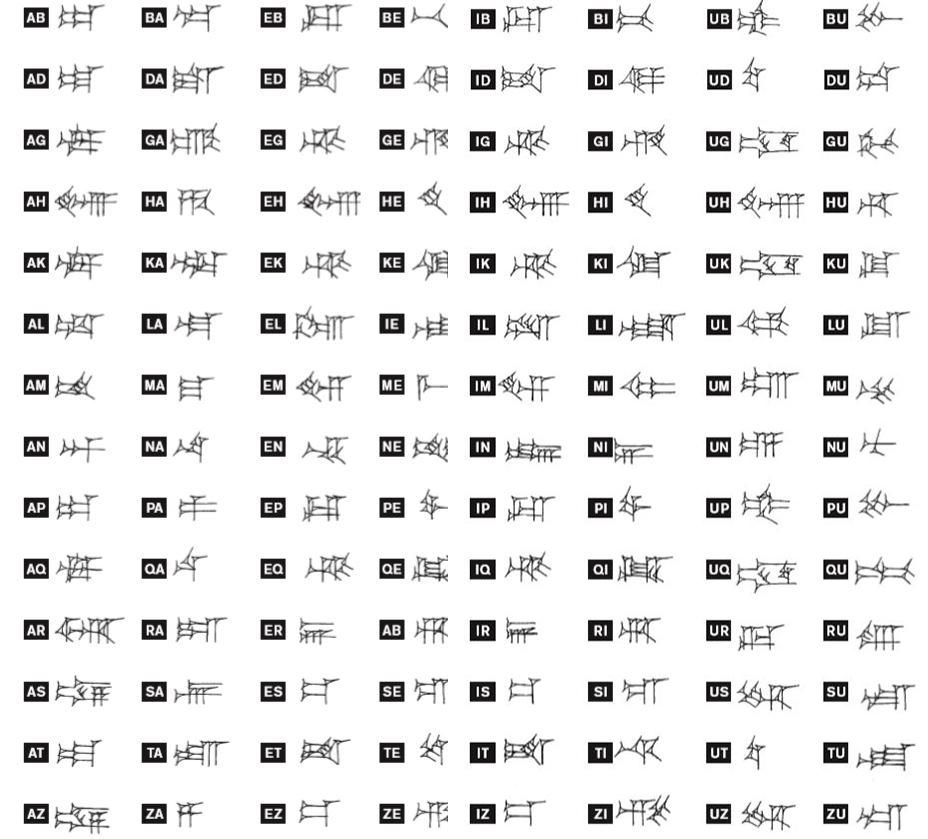
\includegraphics[width=5cm]{Images/cuneiform.jpg}}}%
    \qquad
    \subfloat[\centering World's Earliest Music Composition \\Image from \cite{porter_2018_did} \label{subfig:first_song}]{{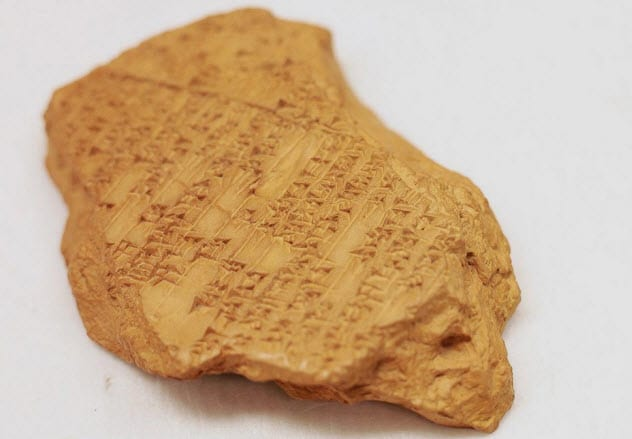
\includegraphics[width=5cm]{Images/first_song.jpg}}}%
\end{figure}
The history of music is extensive and ancient, and it is an essential part of human culture. 
In Syria, a cuneiform "alphabet" (\ref{sub@subfig:cuneiform}) containing the earliest known written composition of music was found (\ref{sub@subfig:first_song}) \cite{porter_2018_did}.
It is thought to have been composed some 3400 years ago. 
The oldest musical instruments, according to archaeological evidence, date back approximately 40,000 years, but the history of music is far older still \cite{killin_2018_the}.
Despite not yet being documented in the archaeological record, these instruments offer a window into far older musical endeavors. 
Proto-musical evolution most likely started about 400,000 years ago, based on the social brain hypothesis \cite{dunbar_social_brain}. 
Musical traditions developed further as people left Africa and spread over the world, reaching a turning point during the Holocene. 
This historical voyage demonstrates the persistent and varied impact that music has played in human history.
Moving forward, there are so many types of music, each representing unique expression of culture, emotion and creativity:
\begin{itemize}
    \item \textbf{Classical Music}: a diverse and evolving tradition, extending beyond the commonly associated period of 1750 to 1820 and encompassing composers from Bach to contemporary artists. 
    It serves as a living and influential force in the world of music, shaping compositions for orchestras, chamber ensembles, solo performers, and even finding unexpected expressions in various genres, from video-game scores to popular music. \cite{gabler_2013_what} \nocite{pentreath_2022_why}
    \item \textbf{Jazz}: originating in early 20th-century New Orleans, is characterized by complex harmony, syncopated rhythms, and a focus on improvisation. 
    Emerging from a rich tradition of ragtime and blues, jazz evolved into a versatile genre that expanded its influence globally, encompassing popular music standards, modal music, and even avant-garde compositions.\cite{beek_2021_what}
    \item \textbf{Blues}: both a musical form and genre, initially associated with melancholy themes, has evolved to encompass a broader range of subjects and emotions, aiming to uplift through music.\cite{chaudhuri_2022_what}
    Characterized by specific chord progressions, a walking bass, call and response, and unique features like microtonality and flattened 'blue' notes, blues is known for its distinct sound and expressive style. \cite{bbc_2023_history}
    \item \textbf{Electronic}: utilizes diverse sound sources, ranging from recorded sounds captured by microphones to those generated by electronic oscillators and complex computer installations. 
    Typically played back through loudspeakers, electronic music can be created using various technologies, with the exception of "live electronic music," which involves real-time performance. \cite{hiller_2019_electronic}
    \item \textbf{Country}: originating in rural Southern and Western areas in the early 20th century, was initially labeled "hillbilly music" before adopting the official term "country and western music" in 1949. 
    Rooted in the ballads, folk songs, and popular tunes of English, Scots, and Irish settlers, country music gained commercial recognition in the early 1920s, marked by its realistic portrayal of rural life contrasting with the sentimental tone prevalent in popular music of that era. \cite{_2019_country} \nocite{_2021_country}
    \item \textbf{Hip-Hop}: a cultural movement that gained widespread popularity in the 1980s and '90s, serves as the foundational music for rap—a style featuring rhythmic and/or rhyming speech, which became the movement's enduring and influential art form. 
    Hip-hop, beyond its musical dimension, encompasses diverse elements such as graffiti art, breakdancing, and social activism, reflecting a multifaceted expression of urban culture and creativity. \cite{tate_2019_hiphop} \nocite{seanmccollum_2019_hiphop}
    \item \textbf{Rock}: a form of popular music that emerged in the 1950s and by the end of the 20th century became the dominant global music genre, influencing the recording industry, international retail, and radio and television playlists. 
    While dictionary definitions often focus on its strong beat and instrumentation, the cultural significance of rock lies in its social and ideological distinctions from other music genres, particularly its development as a term to distinguish certain attitudes and practices from those associated with pop music.\cite{frith_2018_rock}
\end{itemize}

\subsection{Music and Emotion}
Since ancient times, people have been fascinated by the paradoxical connection that exists between music and emotion.
Even though music is an abstract art form that appears to be removed from everyday life, it has a profound potential to evoke strong emotional responses.
This ability of music to trigger strong emotions is also demonstrated in other social circumstances, such as advertising. 
This encounter is further enhanced by the relationship that exists between music and our individual life experiences.
Emotions, influenced by these encounters, provide our perception and thought processes a personalized meaning that connects the abstract quality of music to the concrete events of our everyday life. 
This complex tapestry that highlights the profound influence of music on our emotional environment is created by the blending of music, emotion, and human experience \cite{juslin_2013_music}.
\\
\indent Numerous musical elements that have been thoroughly explored are combined to convey emotions through music. 
Pace, mode, harmony, interval, rhythm, sound level, timbre, timing, articulation, accents, tone attacks and decays, and vibrato are some of these characteristics. 
Emotion in music is expressed through compositional elements as well as performance elements. 
Still, it's not an easy task to express feelings through music. 
Certain musical elements can be employed to convey a range of moods, showing that certain elements are not always reliable predictors of a certain emotion. 
The Lens Model \cite{juslin_2013_music}, which characterizes emotional expression in music as involving probabilistic and partially redundant auditory cues, sheds more light on this complexity.
Listeners combine several cues for successful emotion recognition, and the redundancy of cues allows for a high level of emotion recognition through different combinations, offering room for creativity and personal expression \cite{pereira_2011_music}.
\section{Artificial Intelligence and Machine Learning}
\subsection{Artificial Intelligence}
\gls{ai} is a broad field that includes using technology to build machines and computers that can replicate cognitive abilities connected to human intellect. 
These abilities include making recommendations, language understanding, data processing, and visual perception.
\gls{ai} should be viewed as a group of technologies incorporated into systems rather than as a stand-alone system that can understand, learn, and respond to complex problems.

\subsection{Machine Learning}
\gls{ml} is a branch of \gls{ai} focused on enabling machines and systems to learn and enhance their performance through experience. 
Instead of relying on explicit programming, machine learning employs algorithms to analyze vast datasets, derive insights, and subsequently make informed decisions. 
These algorithms continually improve their performance as they are exposed to more data. The outcomes of this learning process are the machine learning models, which become more proficient with increased exposure to data.

\subsection{Machine Learning Algorithms}
\subsubsection{Linear Regression}
\nocite{mali_2021_linear}
\nocite{rohithgandhi_2018_introduction}
\nocite{kwiatkowski_2021_gradient,ibm_what}
\nocite{_2019_descending}
\gls{lr} is a supervised learning algorithm used to model the relationship between a dependent variable (target) and one or more independent variables (features).
The fundamental assumption of \gls{lr} is that there exists a linear relationship between the input variables and output. \cite{ibm_2022_about}
\begin{equation} \label{eq:linear_equation}
    y = mx + b
\end{equation}
\begin{equation} \label{eq:linear_regression}
    Y = \beta_0 + \beta_{1}X_{1} + \beta_{2}X_{2} + \cdots + \beta_{n}X_{n} + \epsilon
\end{equation}
\indent A \gls{lr} model can be represented by the equation \ref{eq:linear_regression} where $Y$ represented the dependent variable. 
$\beta_0$ is the y-intercept, $\beta_1, \beta_2, \cdots, \beta_3$ are the coefficients  and the $\epsilon$ is an error term, representing the unobserved factors that affect $Y$ but are not accounted for by the model.
The logic of it is same as Linear Equation (\ref{eq:linear_equation}) where using the gradient of the line ($m$), the value of $x$ and the y-intercept ($b$) to get the value of $y$, which is what we are trying to predict. 
\\
\begin{figure}[!ht]
    \centering
    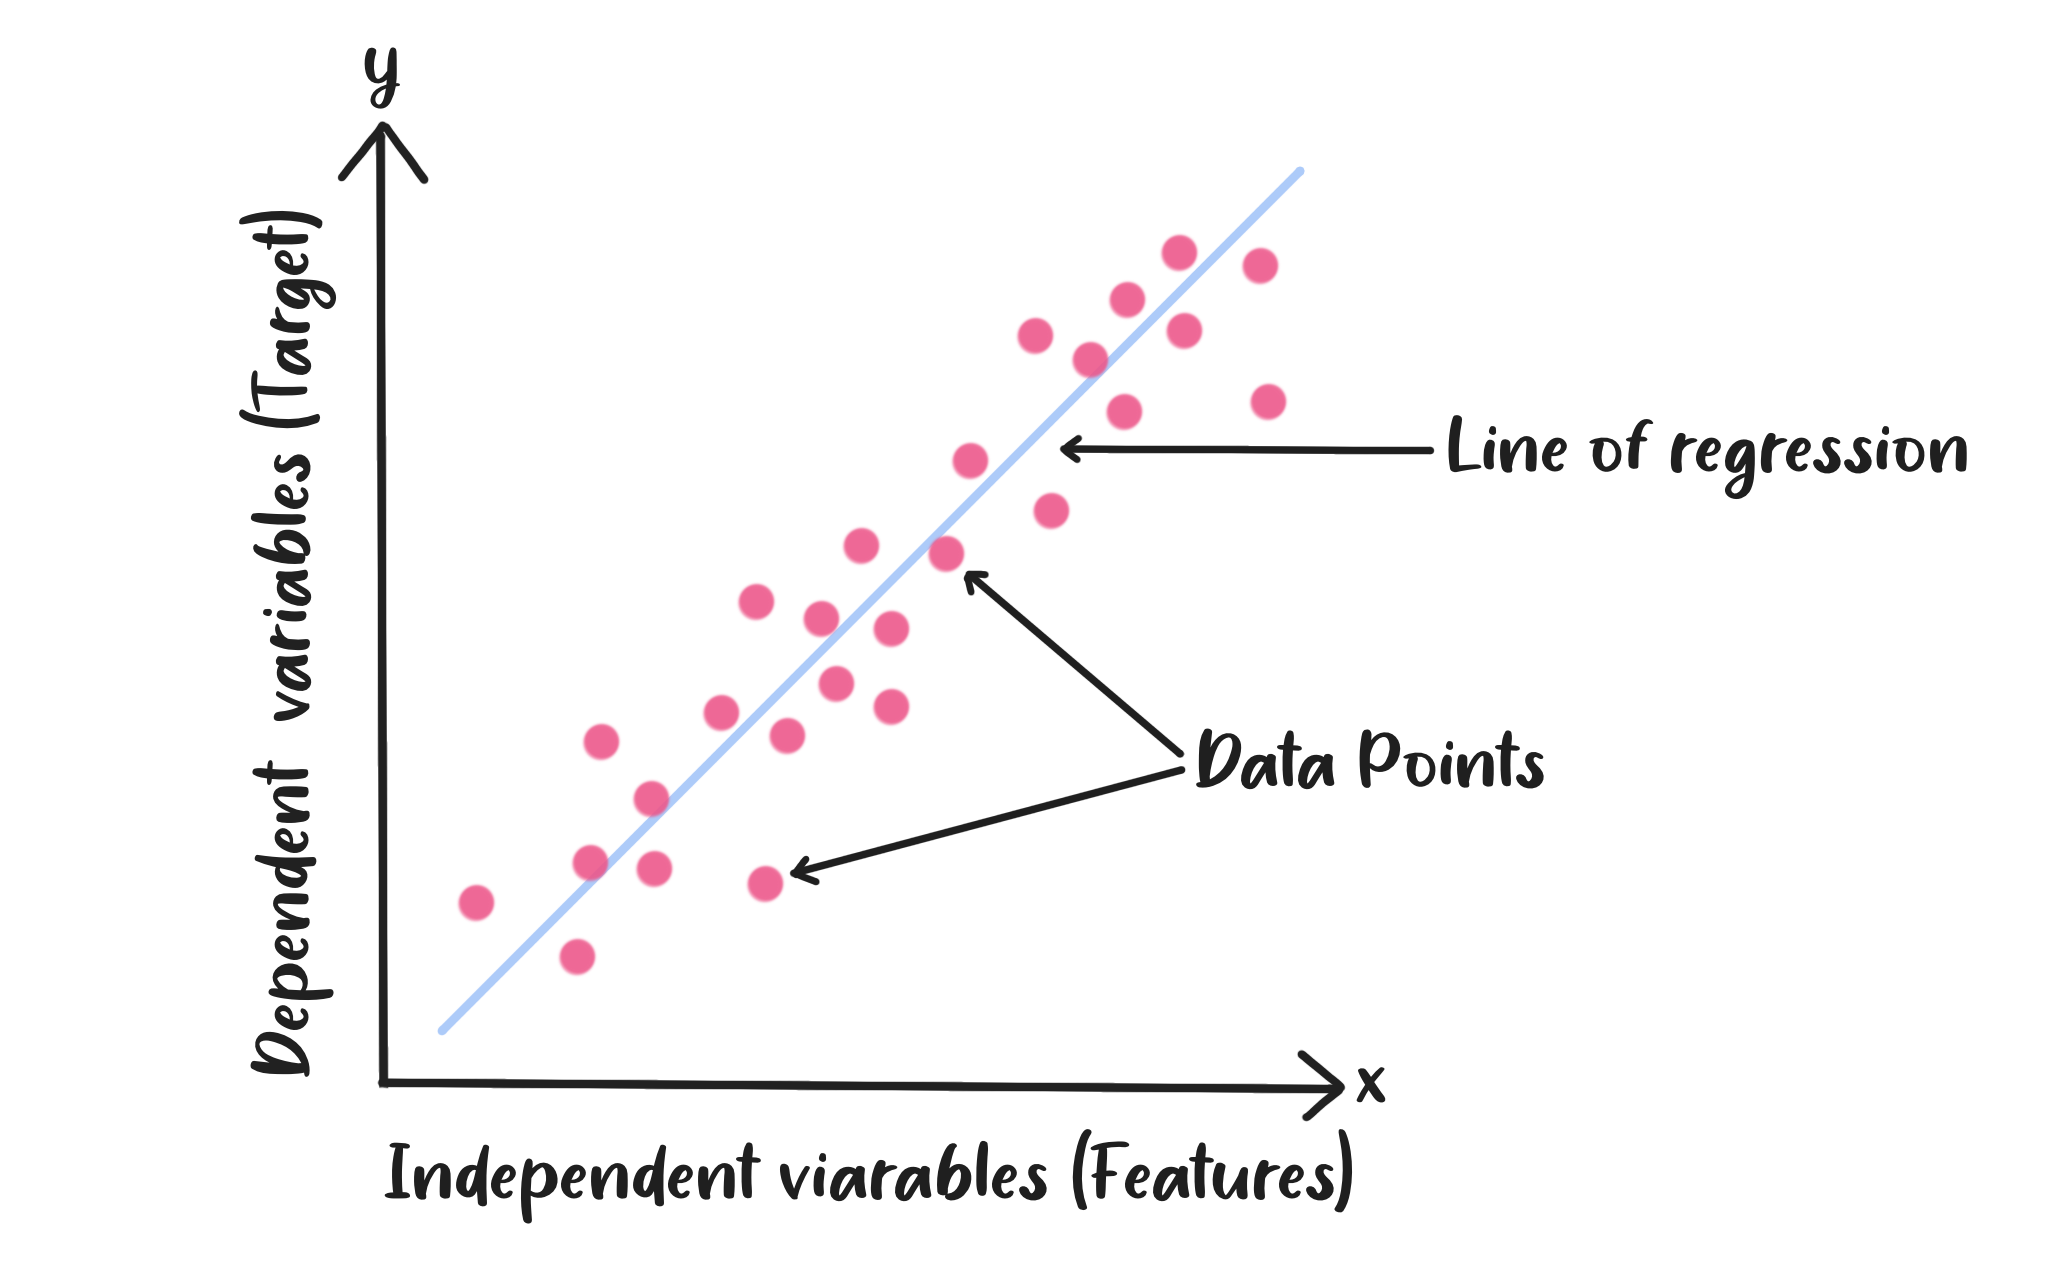
\includegraphics[width=10cm]{Images/lr.png}
    \caption{Linear Regression}
    \label{fig:lr}
\end{figure}
\\
\indent While using \gls{lr}, the main objective is to find the values of $\beta_0, \beta_1,...,\beta_n$ that minimize the error between the predicted value ($\hat{Y}$) and the actual value ($Y$) in the training data.
\\
\begin{equation} \label{eq:mse}
    \text{MSE} = \frac{1}{n} \sum_{i=1}^{n} (Y_i - \hat{Y}_i)^2
\end{equation}
\\
Therefore, \gls{mse}, a cost function to measures the average squared difference between $\hat{Y}$ and $Y$, is introduced to quantify the goodness of fit of the model to the training data. 
If the current result is not optimized, \gls{gd}, an optimization algorithm, will be used to adjust the coefficients, $\beta_0, \beta_1,...,\beta_2$, towards the direction that minimizes the \gls{mse} until it reach the convergence (Figure \ref{fig:gd}).
\\
\begin{figure}[!ht]
    \centering
    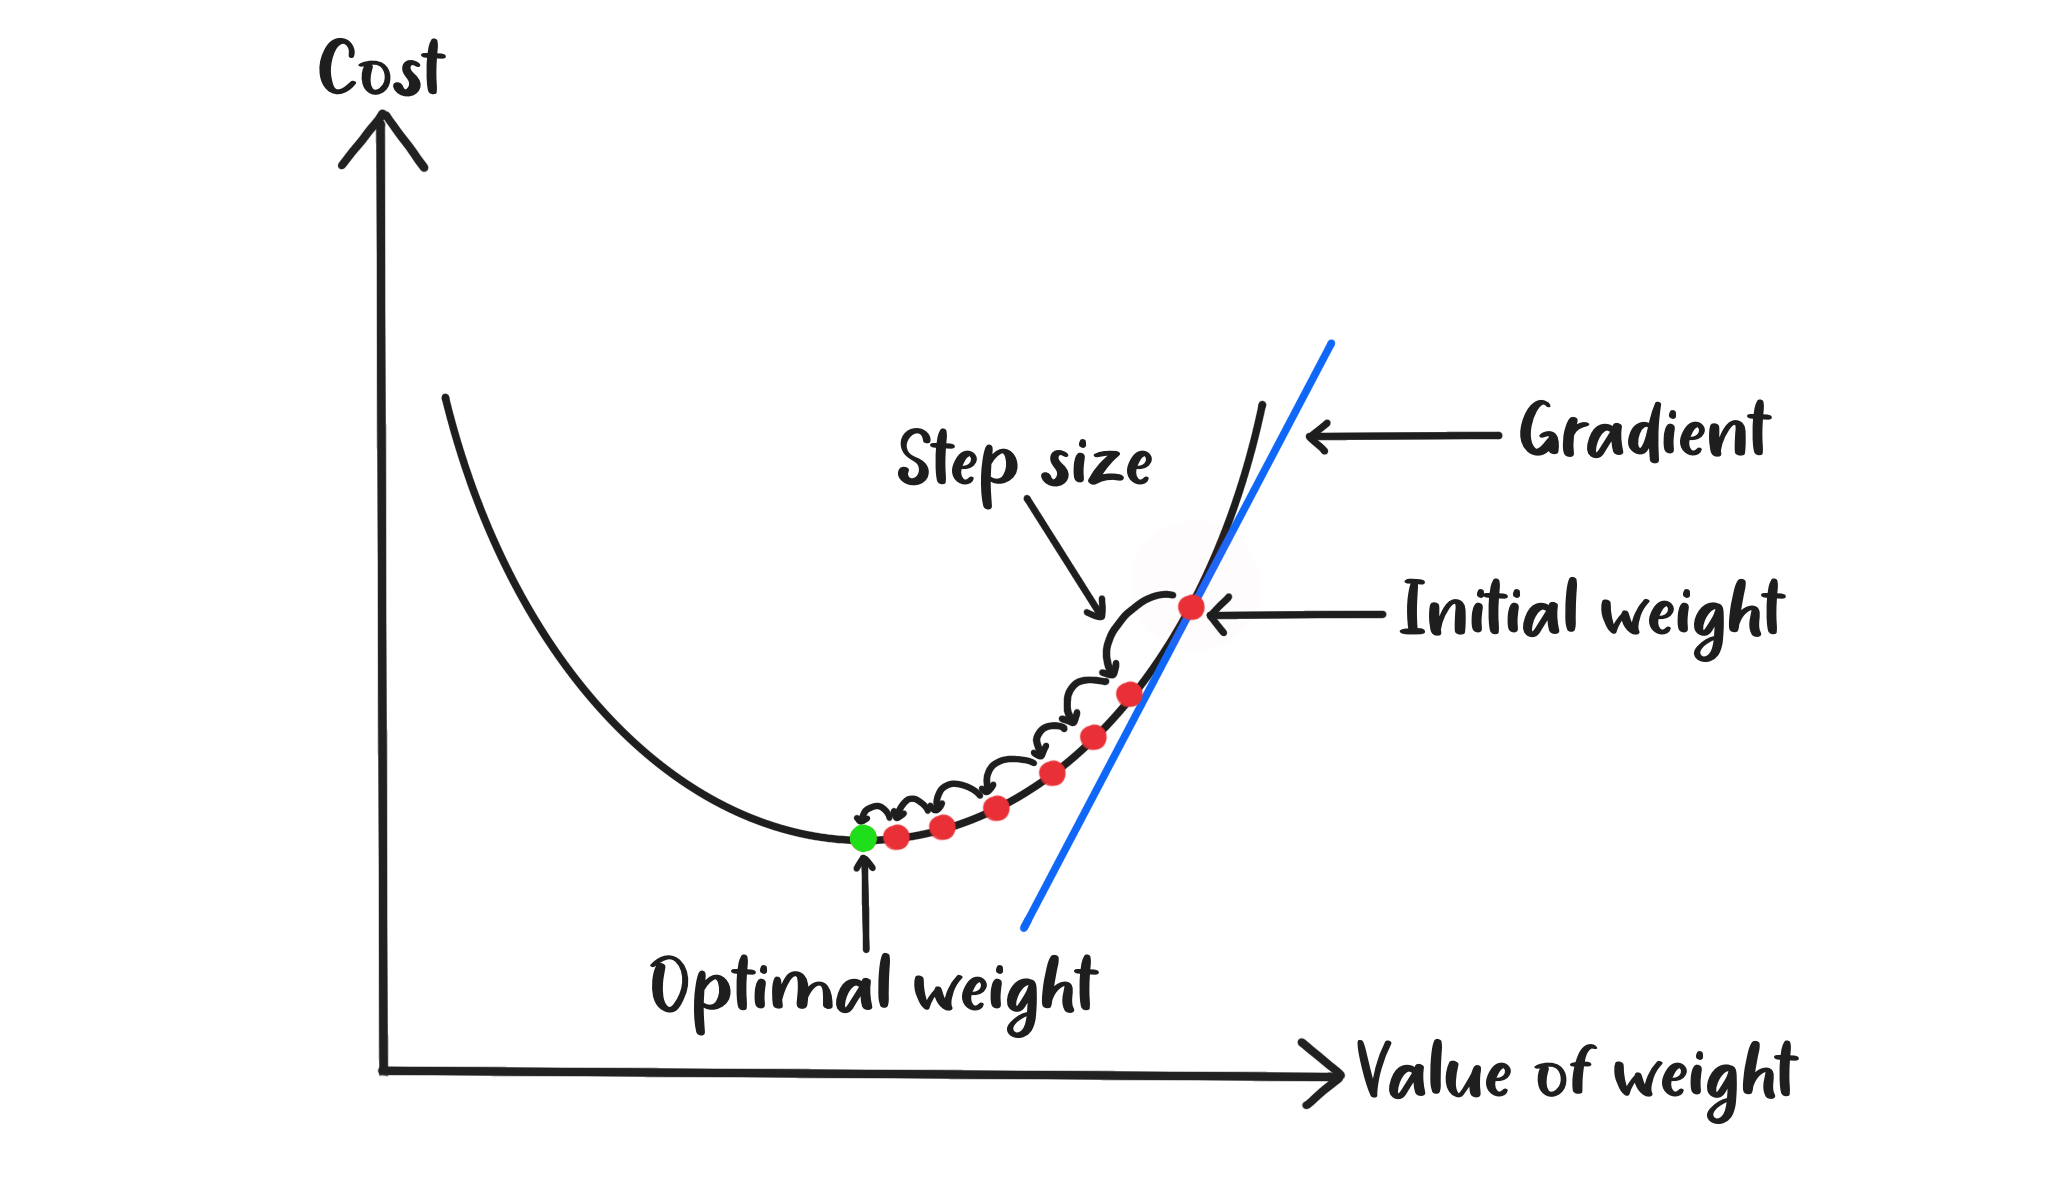
\includegraphics[width=10cm]{Images/gd.png}
    \caption{Gradient Descent}
    \label{fig:gd}
\end{figure}
\\
\subsubsection{Support Vector Machine}
\nocite{berwick_an}
\nocite{_14}
\nocite{saini_2021_support}
\gls{svm} is a supervised \gls{ml} algorithm where we used for classification, regression and outliers detection.
The main goal of it is to find the hyperplane that best separates the data into different classes based on statistical approaches. \cite{gron_2019_handson}
\\
\begin{figure}[!ht]
    \centering
    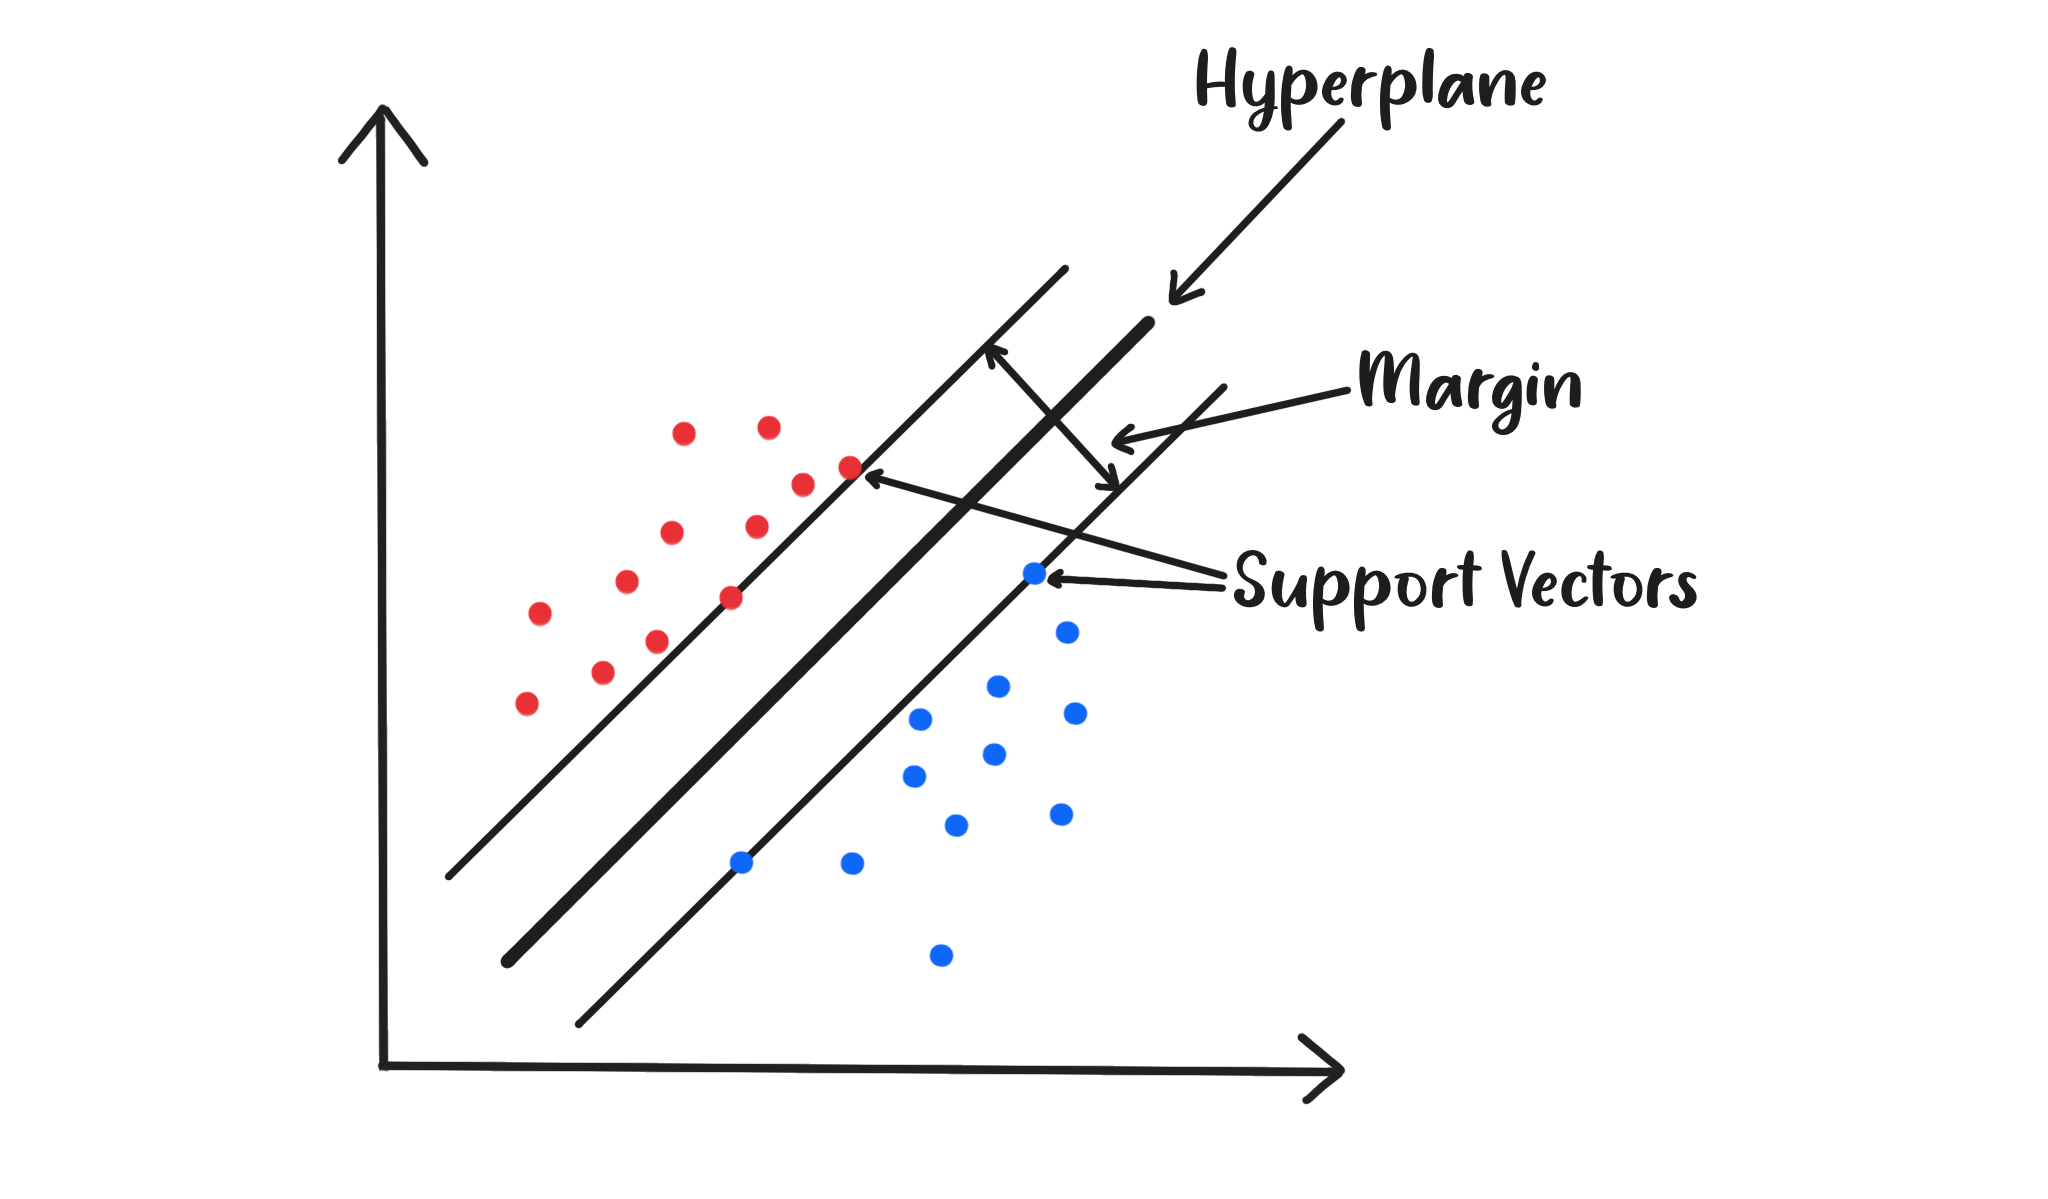
\includegraphics[width=10cm]{Images/svm.png}
    \caption{Support Vector Machine}
    \label{fig:svm}
\end{figure}
\\
\indent While using \gls{svm}, the greater the margin, the better the result would be as it has better generalization to new or unseen data. 
There are two types of \gls{svm} for classification, which are Linear \gls{svm} and Non-linear \gls{svm}.
A linear \gls{svm} finds the optimal hyperplane that maximizes the margin between classes for linearly separable data as Figure \ref{fig:svm}.
\\
\begin{equation} \label{eq:linear_svm}
    f(x) = \text{sign}(\mathbf{w} \cdot \mathbf{x} + b)
\end{equation}
\\
The decision function of linear \gls{svm} (Equation \ref{eq:linear_svm}) is used to defines the ability to classify data points into different classes.
When the result is greater than or equal to zero, the prediction would be positive. If $f(x)$ is less than zero, the decision function predicts the negative class. 
\begin{figure}[!ht]
    \begin{minipage}{0.45\linewidth}
        \begin{equation}
            f(x) = \text{sign}(\sum_{i=1}^{n} \alpha_{i}y_{i}K(x,x_{i}) + b) \label{eq:non_linear_svm}
        \end{equation}
    \end{minipage}
    \hfill
    \begin{minipage}{0.45\linewidth}
        \begin{equation}
            K(x,x_{i}) = (x \cdot x_{i} + c)^{d} \label{eq:poly_svm}
        \end{equation}
    \end{minipage}

    \begin{minipage}{0.45\linewidth}
        \begin{equation}
            K(x,x_{i}) = \text{exp}(-\frac{\parallel x - x_{i} \parallel ^ {2}}{2 \sigma ^ {2}}) \label{eq:rbf_svm}
        \end{equation}
    \end{minipage}
    \hfill
    \begin{minipage}{0.45\linewidth}
        \begin{equation}
            K(x,x_{i}) = \text{tanh}(\alpha x \cdot x_{i} + c) \label{eq:sigmoid_svm}
        \end{equation}
    \end{minipage}
\end{figure}
\\
\indent For non-linearly separable data, \gls{svm} uses kernel functions such as polynomial, sigmoid and radial basis function (RBF), to map the data into a higher-dimensional space where hyperplane can separate the classes.
The equation \ref{eq:non_linear_svm} is the decision function of non-linear \gls{svm}. 
The kernel function, denoted by $K(x,x_{i})$ in the equation, would be replaced by equation \ref{eq:poly_svm} if a polynomial kernel were used.
Similar with the other kernels, if the RBF kernel is employed, it would be exchanged with equation \ref{eq:rbf_svm}, and for sigmoid kernel, it would be replaced with equation \ref{eq:sigmoid_svm}.

\subsubsection{Random Forest}
\nocite{er_2021_random}
\nocite{scikitlearn_2018_sklearnensemblerandomforestclassifier}
\nocite{yiu_2019_understanding}
\gls{rf} is an ensemble learning algorithm that belongs to the family of decision tree-based methods.
A group of decision trees that have been trained on various dataset subsets make up the forest of \gls{rf}, and the final result is derived from averaging the predictions of each individual tree. \cite{ibm_2023_what}
\\
\begin{figure}[!ht]
    \centering
    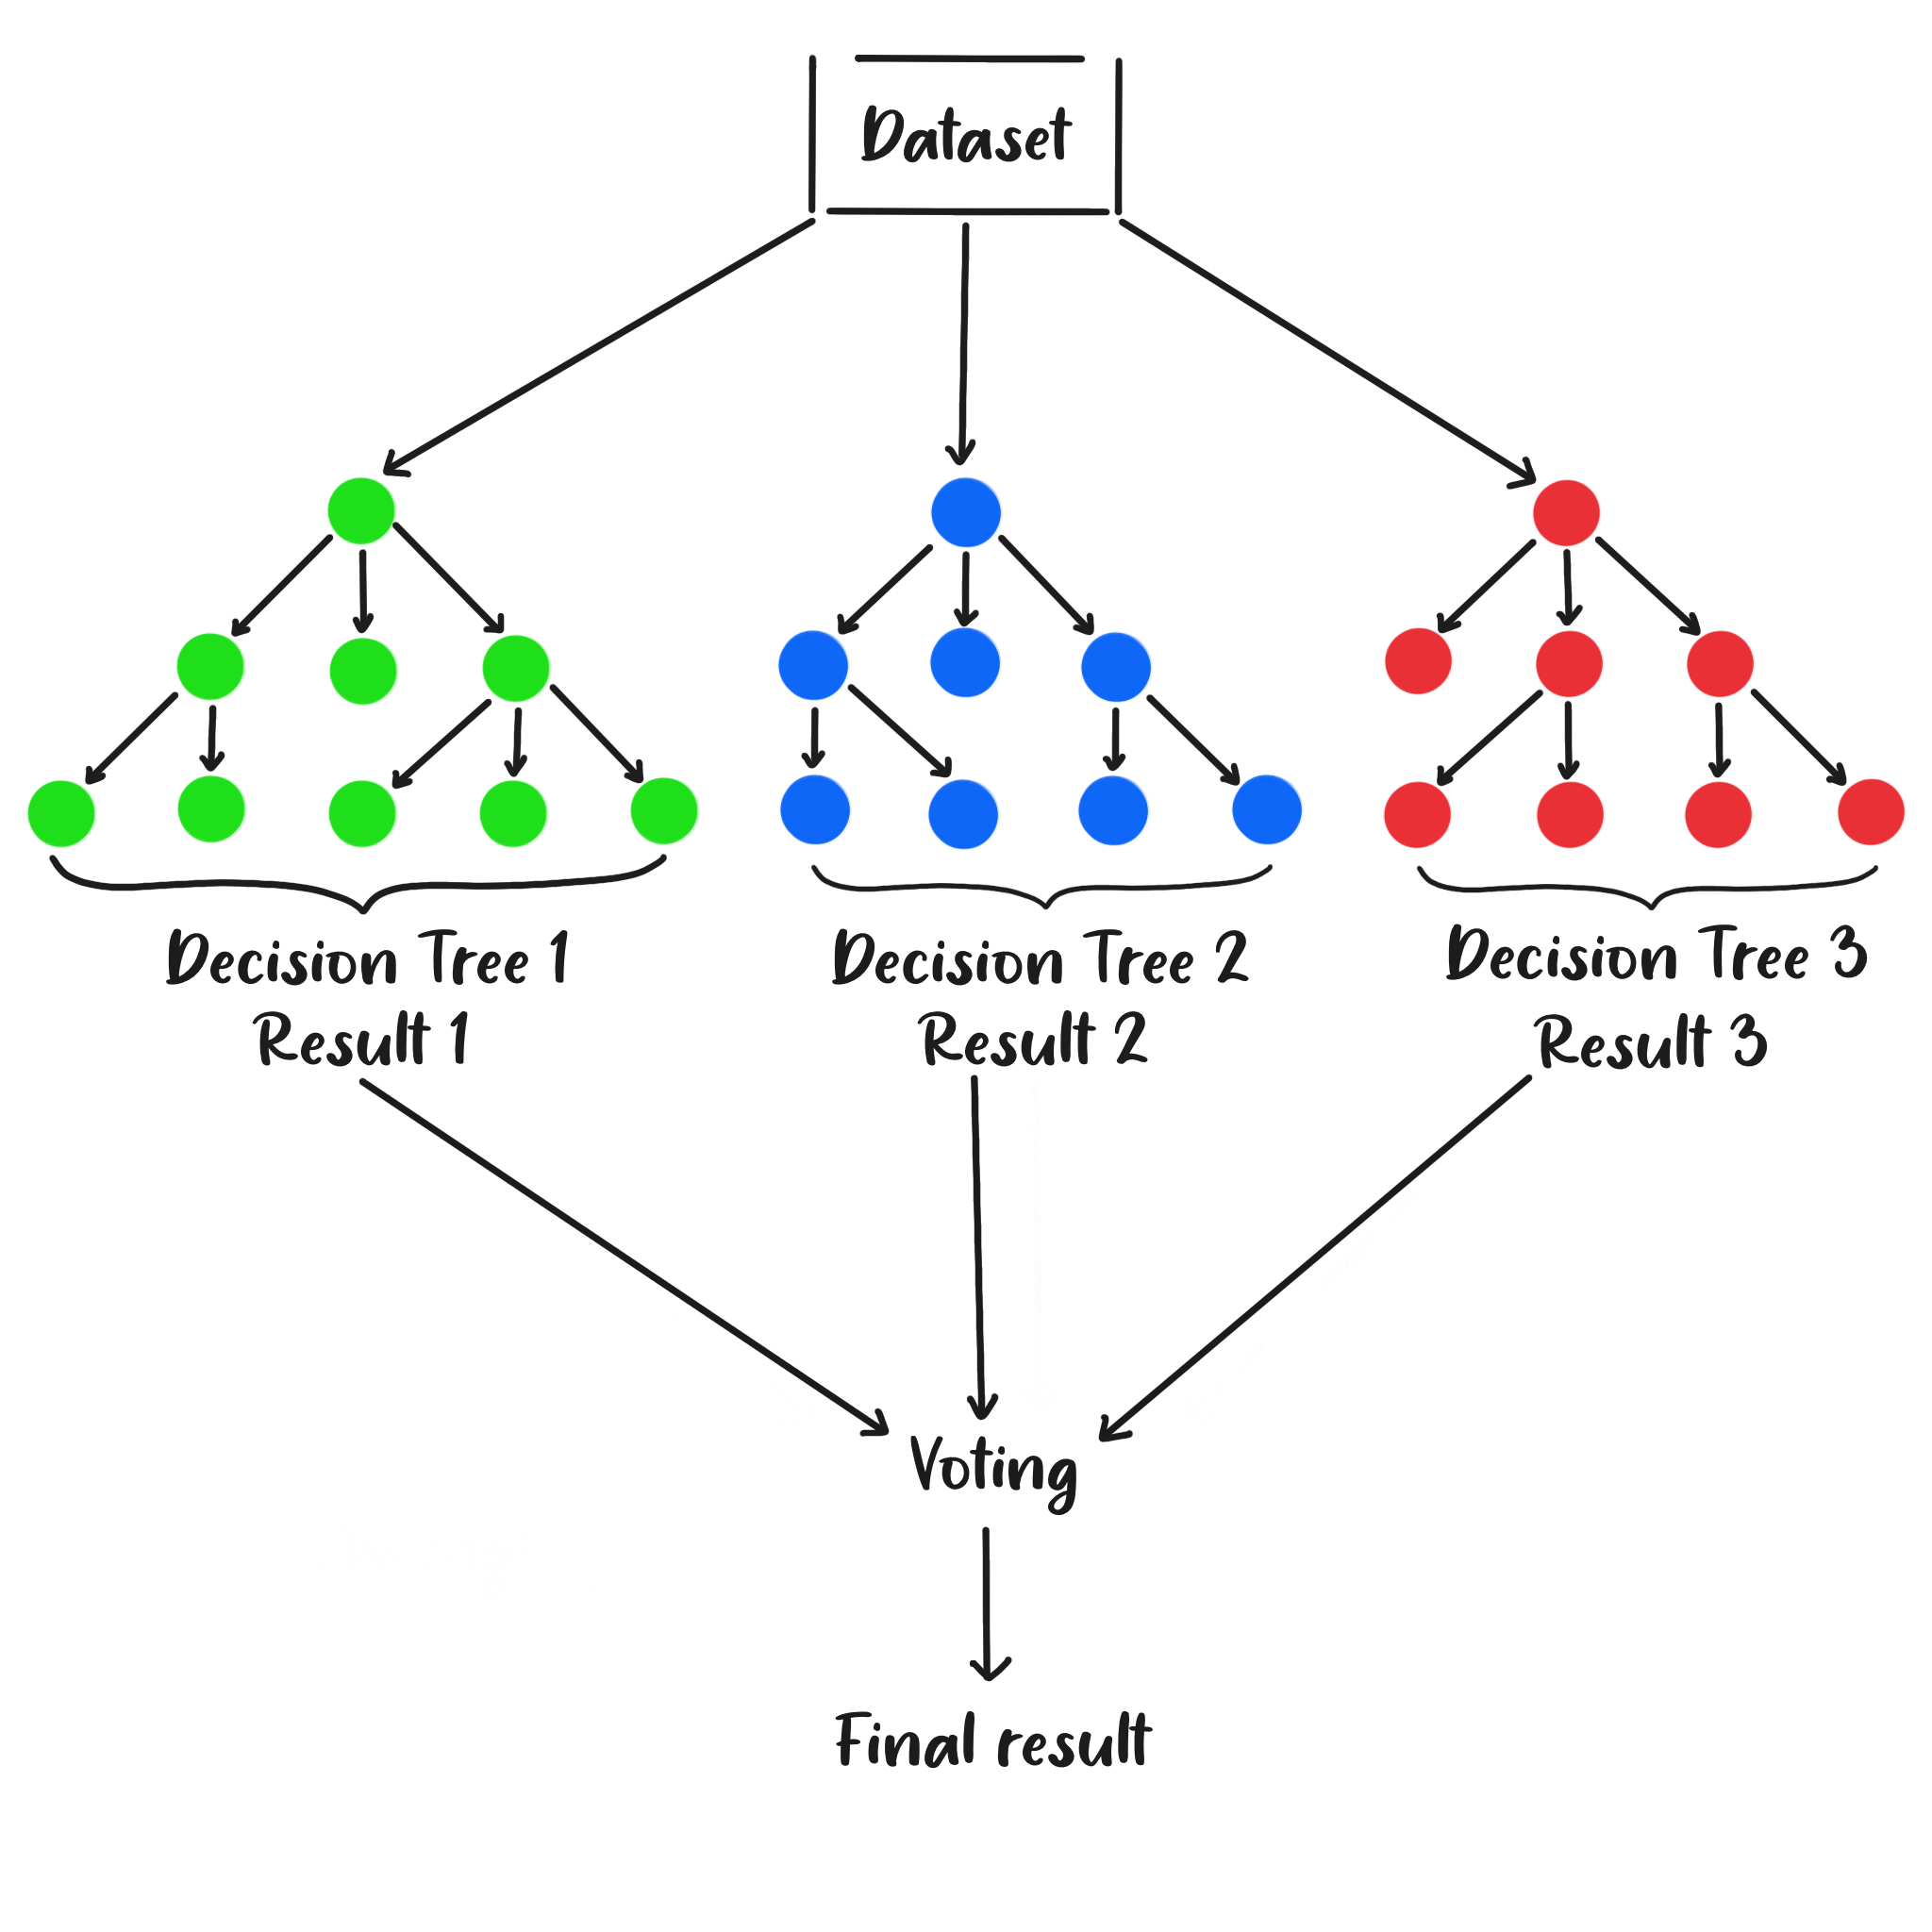
\includegraphics[width=10cm]{Images/rf.png}
    \caption{Random Forest}
    \label{fig:rf}
\end{figure}
\\
\indent As Figure \ref{fig:rf} shown, \gls{rf} builds multiple Decision Trees and combines them to get a more accurate and stable prediction than any individual model.
This process is called bagging which is one of a type of ensemble learning. 
In the process, the entire dataset is separated into subsets and each decision tree is trained individually on a subset that is selected at random.
This adds variety and unpredictability to the trees.
The training process will then generate results for each model, and the final output is determined by the "votes" for a class from each tree.
The class with the majority of votes is chosen as the final prediction.
\subsubsection{K-Nearest Neighbors}
\nocite{srivastava_2019_introduction}
\nocite{geeksforgeeks_2018_knearest}
\nocite{harrison_2018_machine}
\gls{knn} is a intuitive supervised machine learning method used for both classification and regression tasks. 
The main idea of \gls{knn} is to predict the label of new data point based on its k-nearest data points in the feature space. \cite{ibm_what_knn}
\\
\begin{figure}[!ht]
    \centering
    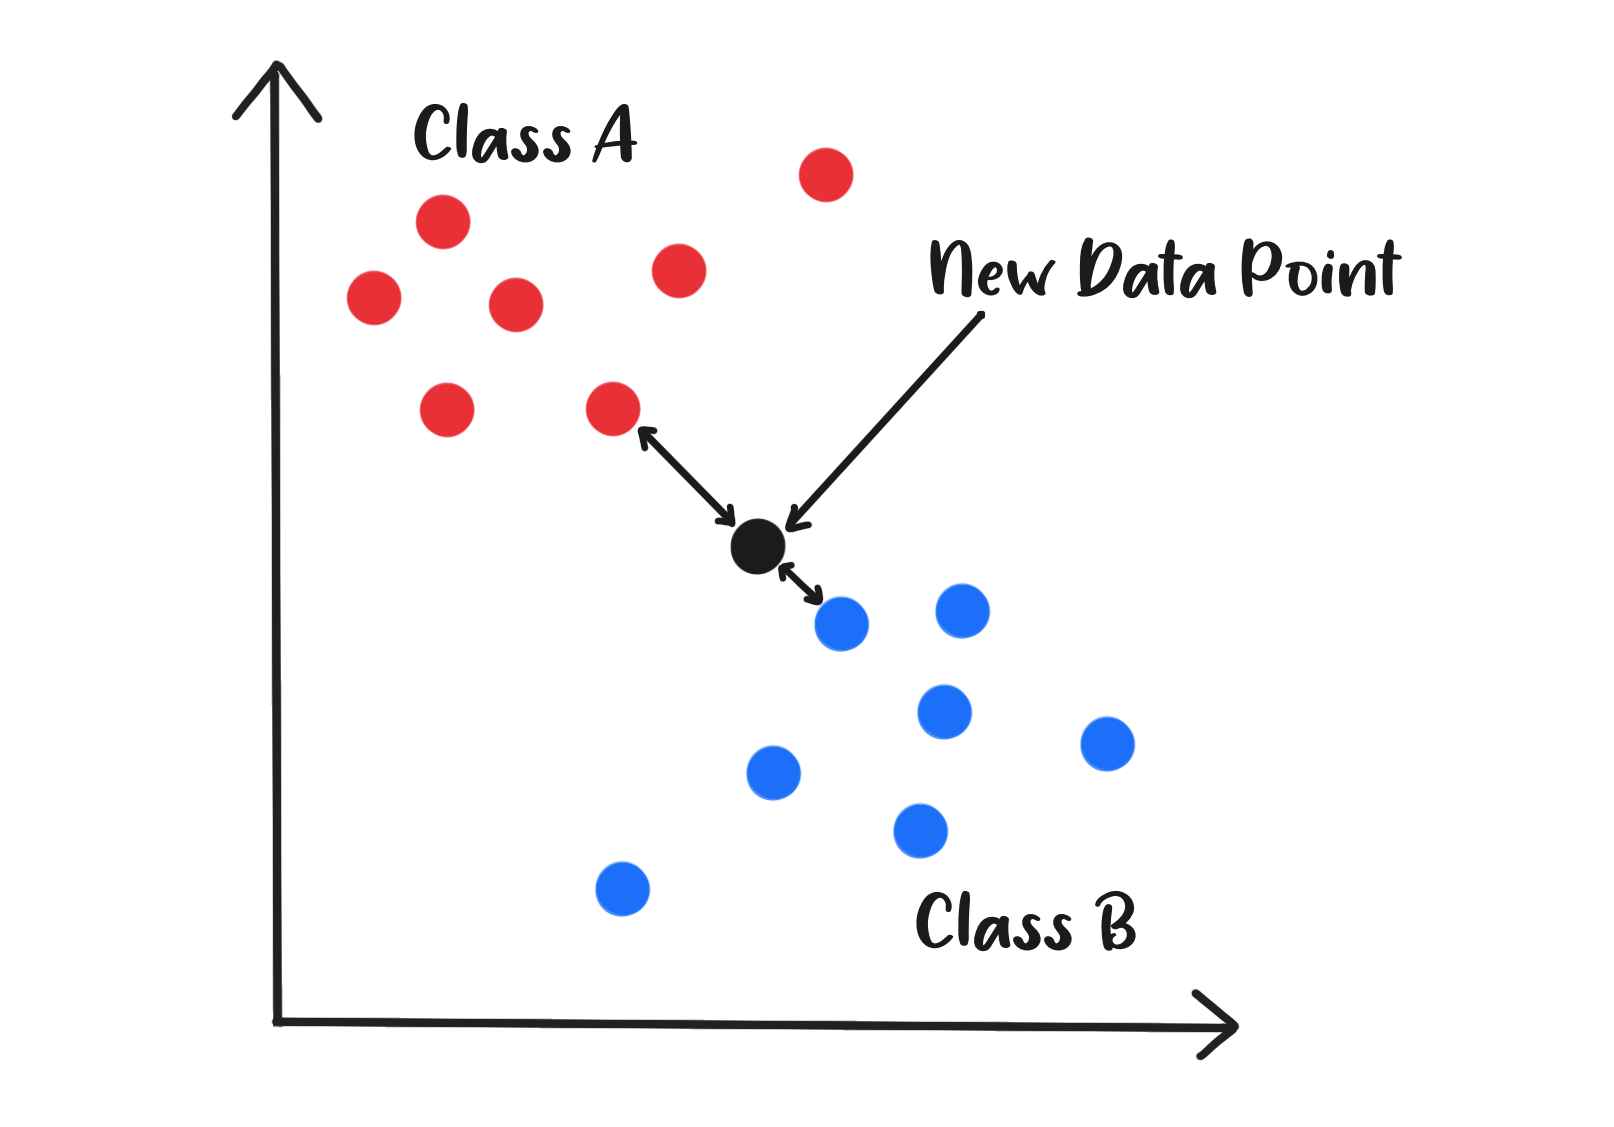
\includegraphics[width=10cm]{Images/knn.png}
    \caption{K-Nearest Neighbors}
    \label{fig:knn}
\end{figure}
\\
\indent \gls{knn} uses distance metric (Equation \ref{eq:euclidean}) to calculate how similar two data points are to one another.
\gls{knn} finds the k training data points that, according to the selected distance metric, are closest to a given data point.
In classification tasks, the majority class among a new data point's k-nearest neighbors predicts the class that the data point will fall into.
\\
\begin{equation} \label{eq:euclidean}
    d(P,Q) = \sqrt{\sum_{i=1}^{n}(p_{i} - q_{i})^{2}}
\end{equation}
\begin{equation} \label{eq:knn}
    \hat{Y} = \text{argmax}_y \left( \sum_{i=1}^{k}I(y_{i}=y) \right)
\end{equation}
\\
\indent The key hyperparameter of \gls{knn} is the value of $k$ (Equation \ref{eq:knn}), representing the number of nearest neighbors to consider.
The choice of $k$ can significantly impact the performance of the algorithm, and it is often selected through cross-validation.

\subsubsection{Neural Networks}
\paragraph{Multi-Layer Perceptron}
\begin{figure}[!ht]
    \centering
    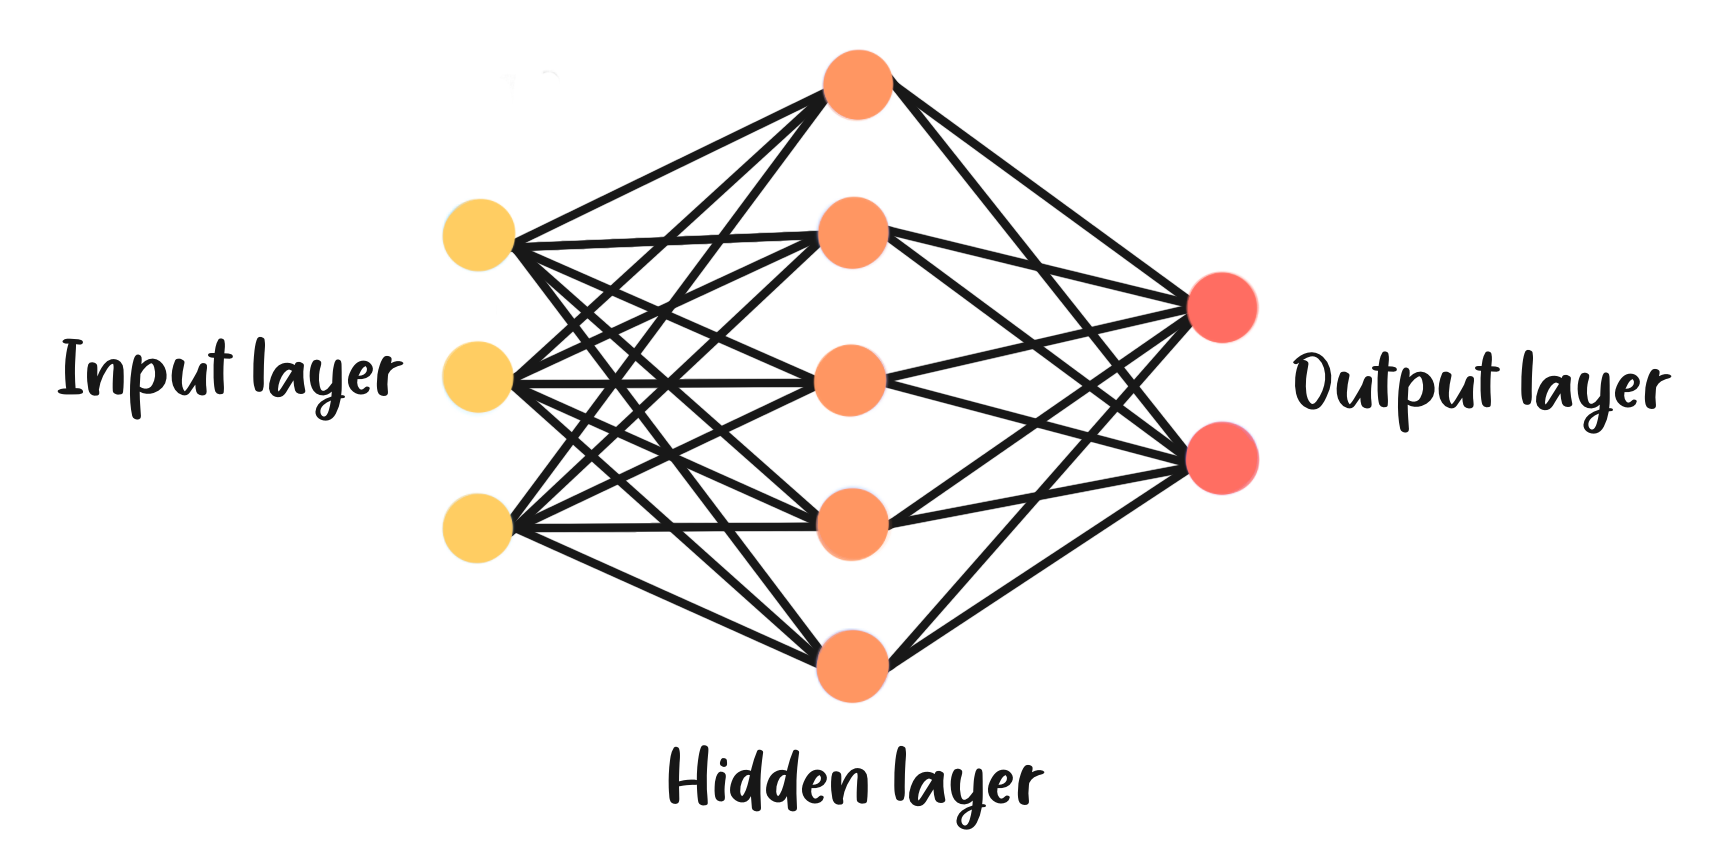
\includegraphics[width=10cm]{Images/mlp.png}
    \caption{Multi-Layer Perceptron}
    \label{fig:mlp}
\end{figure}
An input layer, one or more hidden layers, and an output layer are the minimum number of nodes that make up a \gls{mlp} feedforward artificial neural network type (Figure \ref{fig:mlp}).
All nodes in these layers—aside from those in the input layer—are linked using a specific weight and employ a nonlinear activation function.
Because of its nonlinearity, the network may learn and carry out more complicated tasks as well as represent intricate connections between the input and output.
A \gls{mlp} model is trained by comparing its output to the expected output and propagating errors back through the network to alter the weights. 
This process is known as backpropagation. \\\cite{haykin_2014_neural}

\paragraph{Convolutional Neural Networks}
\nocite{ibm_2023_what_cnn}
\nocite{mishra_2020_convolutional}
\nocite{mandal_2021_cnn}
\nocite{saha_2018_a}
\gls{cnns} are a family of deep learning algorithms that are mostly utilized for processing input that has a grid structure, like images. \cite{yamashita_2018_convolutional}
\\
\begin{figure}[!ht]
    \centering
    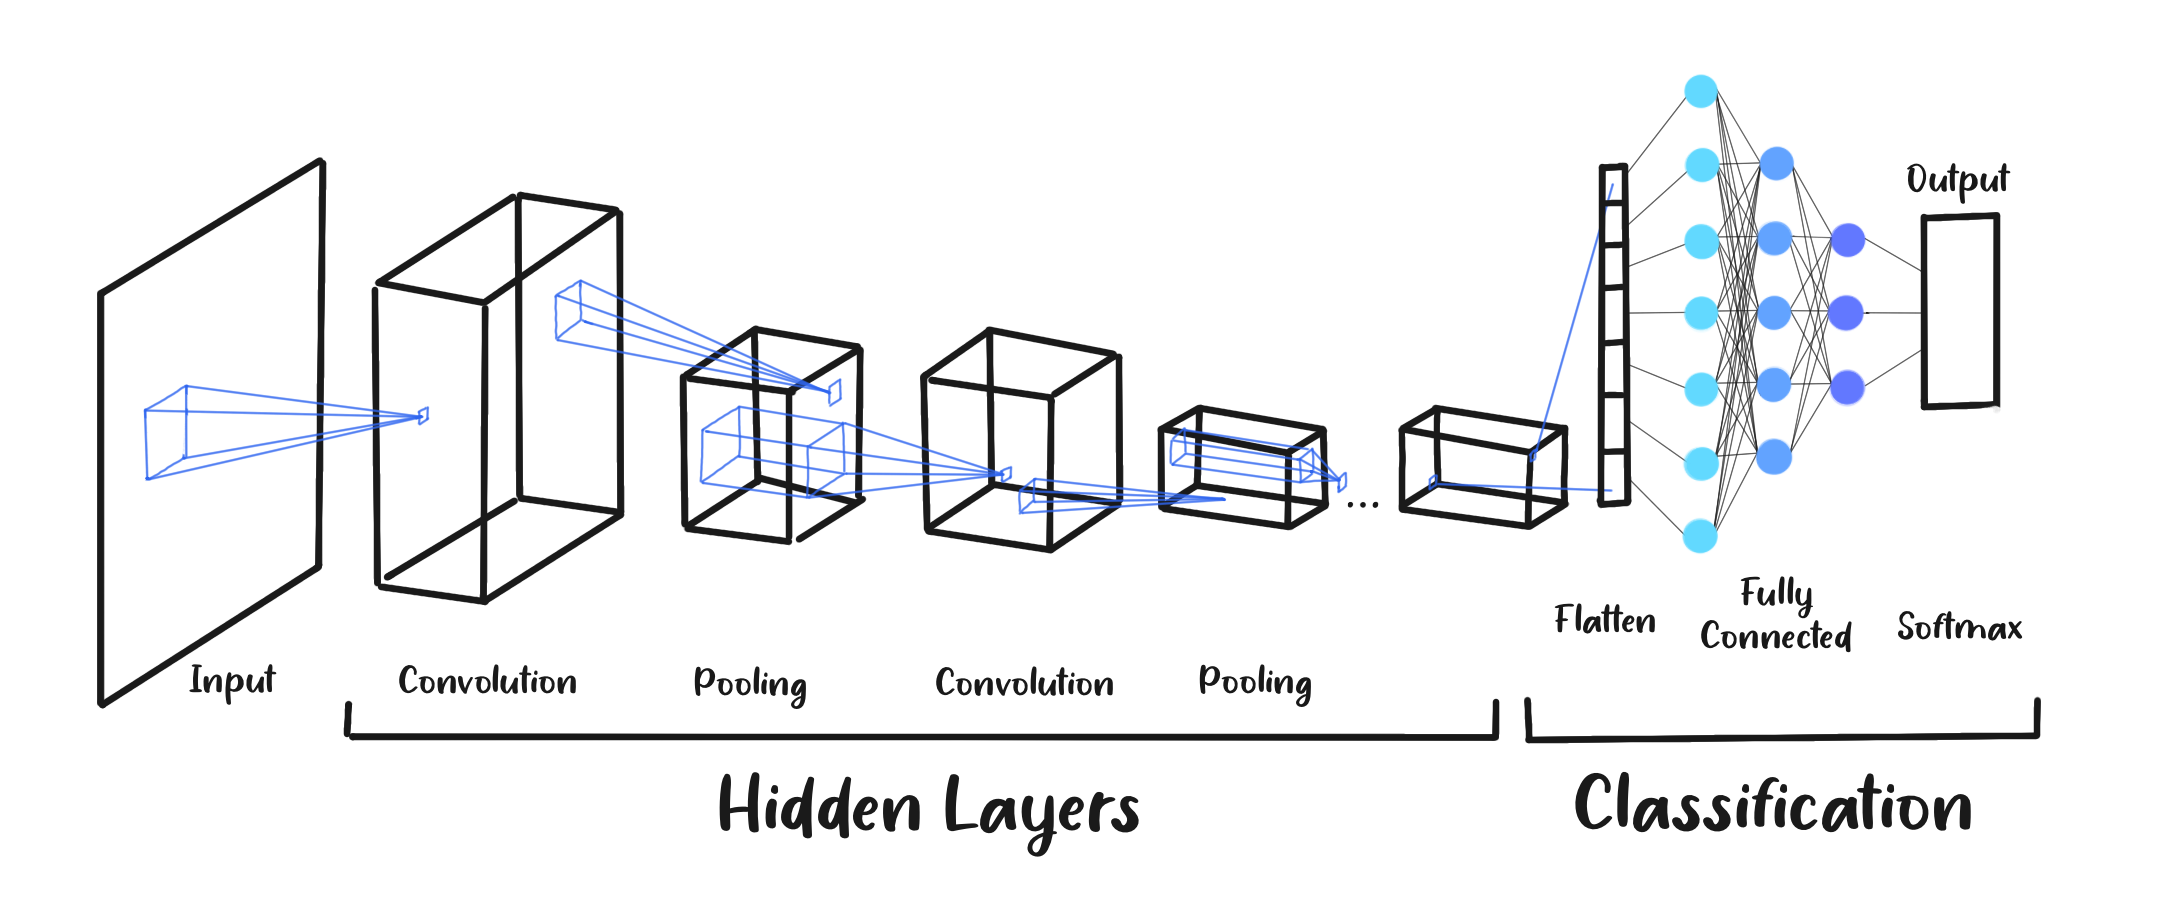
\includegraphics[width=16cm]{Images/cnns.png}
    \caption{Convolutional Neural Networks}
    \label{fig:cnns}
\end{figure}
\\
\indent \gls{cnns} are designed to adaptively learn spatial hierarchies of features from the data. 
This learning process includes convolution layers, pooling layers, flatten layer, and fully connected layers.
By applying filters, also known as kernels, to the input, these layers carry out the convolution process and produce feature maps. 
Local elements like textures and edges are captured throughout this procedure.
Pooling layers, which come after convolutional layers, help to reduce the number of parameters and computation in the network by reducing the spatial dimensions (width and height) of the input volume. 
\\
\indent The features from the input image are retrieved by the convolutional and pooling layers, and the next stage is to categorize the features which is done in flatten layer.
The feature maps are converted into a one-dimensional vector in the flatten layer, which is necessary for fully connected layers.
The flattened vector is then fed into the fully connected layers (which resemble the standard neural network layers with fully connected nodes) for the classification task. 
These fully connected layers divide the image into discrete groups based on the high-level characteristics found in the preceding levels.
\\
\indent The last layer of layers in the network architecture play the crucial job of generating the output.
The output layer typically uses a softmax activation function in multi-class classification settings to translate the network's raw output into probabilities given to each class. 
The output node with the highest probability is then chosen to determine the anticipated class.
\\
\section{Facial Emotion Recognition}
Human emotions can be inferred from facial expressions. 
Deciphering these signs of emotion has become a popular research topic in the fields of Human Computer Interaction and Psychology. \cite{vemou_2021_facial}
The development of \gls{fer} technology has been significantly aided by technological advancements, particularly with the introduction of \gls{ml} and Pattern Recognition.
\\
\begin{figure}[!ht]
    \centering
    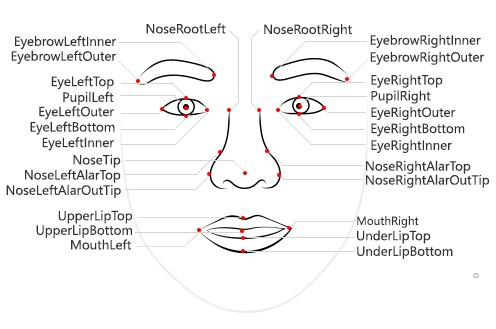
\includegraphics[width=10cm]{Images/landmarks.jpg}
    \caption{Facial Landmarks} \footnotesize{Image from \cite{patrickfarley_2023_face}}
    \label{fig:facial_landmark}
\end{figure}
\\
\indent \gls{fer} is a broad field that intersects with Computer Science, \gls{ai}, Psychology and other fields. 
It involves analyzing a person's facial expressions in still images and videos in order to determine their emotional state. 
A three-step approach is used in the methodology: face detection, facial expression identification, and categorization of the expression into a certain emotional state. 
Facial landmark (Figure \ref{fig:facial_landmark}) detection and analysis of changes in their positions are key components of this complex process. 
\gls{fer} attempts to offer insights into people's emotional experiences by identifying muscular contractions linked to various emotions from visual clues found in facial expressions.
\\
\begin{figure}[!ht]
    \centering
    \subfloat[\centering Confusion Matrix for k-NN Classifier \label{subfig:knn-tarnowski}]{{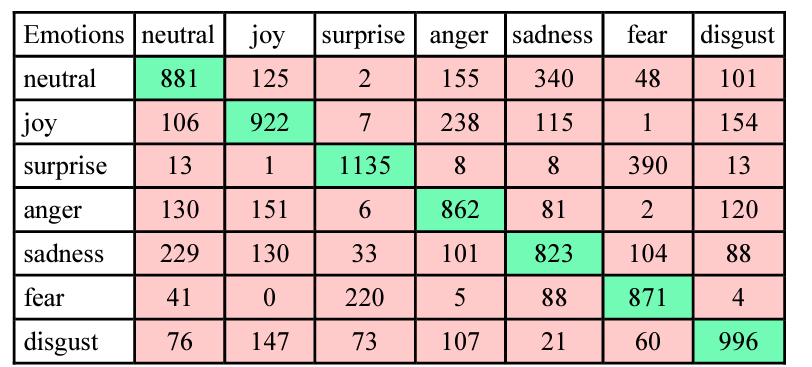
\includegraphics[width=7cm]{Images/fer1stknn.png}}}%
    \qquad
    \subfloat[\centering Consfusion Matrix for MLP Classifier \label{subfig:mlp-tarnowski}]{{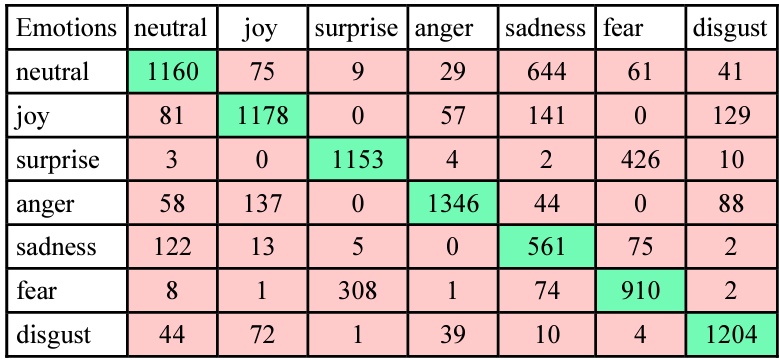
\includegraphics[width=6.7cm]{Images/fer1stmlp.png}}}%
    \vspace{0.5cm}
    \\
    \scriptsize{Tables from \cite{tarnowski_2017_emotion}}
\end{figure}
\\
\indent As stated by Tarnowski et al. (2017), the creative feature extraction from facial expressions using coefficients that detailed aspects of emotional states is what makes the research successful.
They distinguished between seven different emotional states: happiness, sorrow, surprise, wrath, fear, and contempt, as well as the more subdued displays of neutrality. 
For featre computation, they employed a three-dimensional facial model as an alternative to conventional two-dimensional approaches. 
This enables them to collect more detailed and subtle data, which may improve the accuracy of identifying emotions. 
On top of that, they used the MLP neural network and the \gls{knn} classifier to classify each emotional state. 
According to their research and comparative analysis, the MLP is more accurate than the \gls{knn} in classifying emotional states, with a 73\% classification accuracy compare to a 63\% accuracy for \gls{knn} \cite{tarnowski_2017_emotion}.
\\
\indent Mellouk et al. (2020) showed in their study that \gls{fer} may be achieved with great accuracy and effectiveness by utilizing deep learning techniques.
They provided a thorough analysis of multiple \gls{fer} databases, emphasizing their diversity in terms of picture, video content, lightning circumstances, and demographic variances—all of which are important determinants of \gls{fer} performance—in order to guarantee the credibly of the results.
\\
\indent Traditional facial recognition techniques included manually defining and extracting features from facial photos, a procedure that was frequently less flexible and efficient. 
Examples of these techniques include Local Binary Patterns (LBP), Facial Action Coding System (FACS), Local Directional Patterns (LDA), and Gabor wavelet. 
\gls{cnns} and LSTMs can automatically extract and learn complex patterns from facial data, according to Mellouk et al., which will improve the reliability and accuracy of emotion recognition. 
Furthermore, the difficulties that traditional approaches faced—such as variances in facial characteristics due to diverse demographics, occlusions, and data diversity—are resolved with the use of deep learning, increasing their versatility and effectiveness.
The study also examines preprocessing methods including image scaling, cropping, normalization, and data augmentation that are crucial for improving the accuracy of these deep learning models.
\\
\indent With the help of deep learning and the preprocessing techniques they found, the outcome demonstrates proficiency in accurately classifying the fundamental emotions, with some models reaching over 90\% accuracy under specific circumstances \cite{mellouk_2020_facial}. 
It indicates that as machines improve at deciphering human emotions, interactions between humans and machines may become more intuitive and natural.
\\
\begin{figure}[!ht]
    \centering
    \subfloat[\centering Accuracy variation with 32 Filters and 8 kernel size for Model 1 \label{subfig:new_cnn1}]{{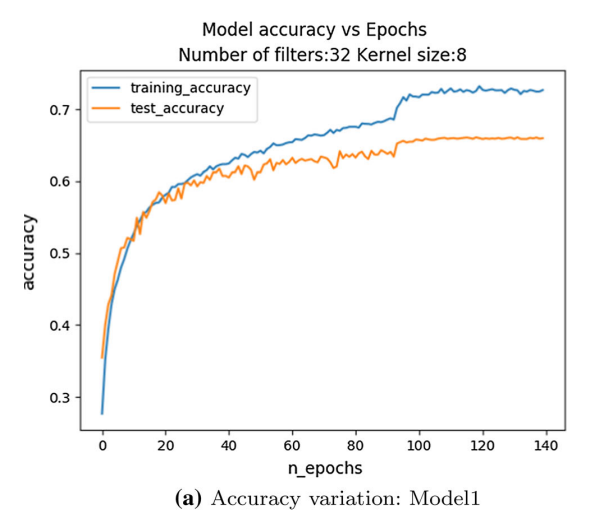
\includegraphics[width=6.8cm]{Images/new_cnn_model1.png}}}%
    \qquad
    \subfloat[\centering Accuracy variation with 32 Filters and 8 kernel size for Model 2 \label{subfig:new_cnn2}]{{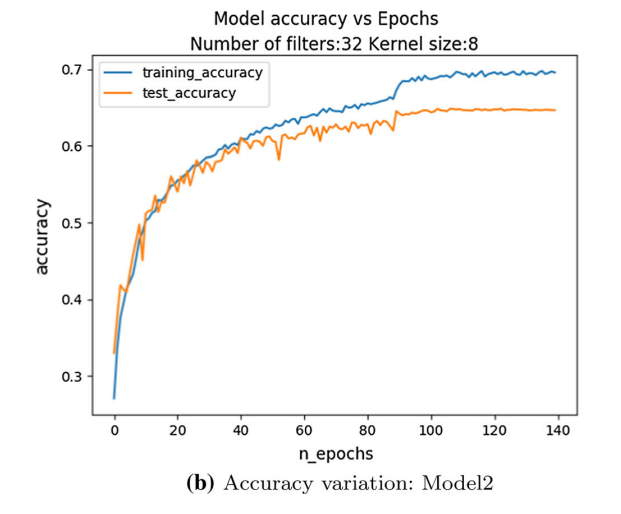
\includegraphics[width=7cm]{Images/new_cnn_model2.png}}}%
    \vspace{0.5cm}
    \\
    \scriptsize{Graphs from \cite{agrawal_2019_using}}
\end{figure}
\\
\indent Based on the findings of Agrawal et al.'s work, the kernel size and the number of filters significantly impact \gls{cnns} accuracy.
Using the FER-2013 dataset as their primary emphasis, two CNN architectures is put forth after a thorough analysis of various kernel sizes and filter counts.
To find the optimal set of parameters that could yield the best convergence and accuracy, Agrawal et al. ran tests with the combination of 6 different kernel sizes (2, 4, 8, ..., 64) and 8 different number of filters (2, 4, 8, ..., 256). 
They discovered that when network depth increased, a network with 32 filters and an 8 kernel size demonstrated a discernible gain in accuracy (Figure \ref{subfig:new_cnn1}, Figure \ref{subfig:new_cnn2}).
\\
\begin{figure}[!ht]
    \centering
    \subfloat[\centering Confusion Matrix for Model 1 \label{subfig:new_cm1}]{{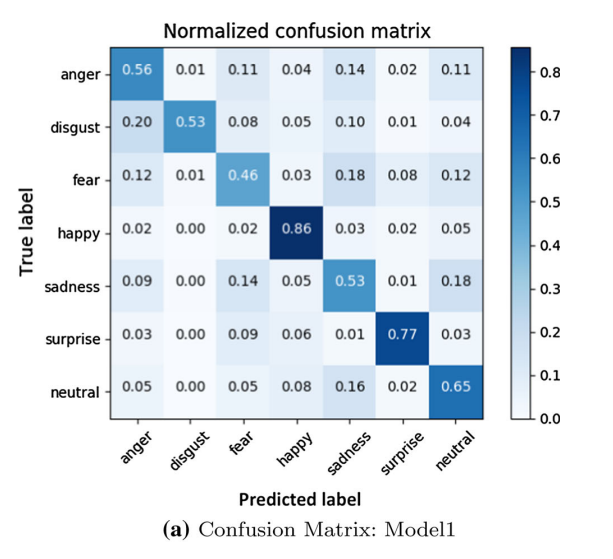
\includegraphics[width=7cm]{Images/new_cnn_cm_1.png}}}%
    \qquad
    \subfloat[\centering Confusion Matrix for Model 2 \label{subfig:new_cm2}]{{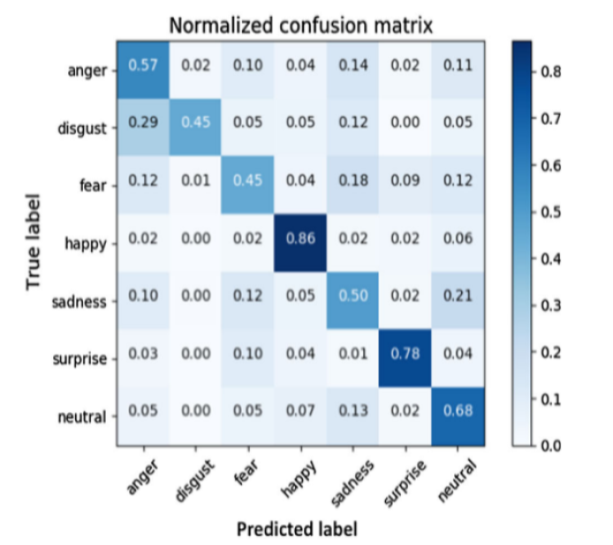
\includegraphics[width=7cm]{Images/new_cnn_cm_2.png}}}%
    \vspace{0.5cm}
    \\
    \scriptsize{Graphs from \cite{agrawal_2019_using}}
\end{figure}
\\
\indent Even while Model 2 is simpler due to its constant kernel size, lack of dropout layers, and fully connected layers, it was nevertheless able to achieve an accuracy of 65\% on the FER-2013 dataset, which is comparable to human performance \cite{agrawal_2019_using}.
Furthermore, in comparison with other emotions, the proposed models were able to categorize happiness and surprise with a higher degree of accuracy, which is consistent with people's challenges in picking out distinct emotions (Figure \ref{subfig:new_cm1}, Figure \ref{subfig:new_cm2}).
\\
\begin{figure}[!ht]
    \centering
    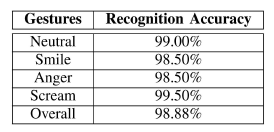
\includegraphics[width=6cm]{Images/lr_result.png}
    \caption{Linear Regression Classification Accuracies Table} \footnotesize{Table from \cite{naseem_2010_linear}}
    \label{fig:lrc_result}
\end{figure}
\\
\indent A pivotal study by Naseem et al. (2010) incorporates the analysis of facial expressions, recognizing them as crucial variations in appearance induced by internal emotions or social communications.
In order to evaluate their \gls{lr} Classification approach, they therefore took into account occlusion modes, brightness changes, and expressions such as scream, smile, rage, and neutral
Notably, the \gls{lr} Classification algorithm showed an excellent recognition accuracy for all facial expressions tested, averaging 98.88\% in a 100D feature space (Figure \ref{fig:lrc_result}). 
For the screaming expression, the algorithm outperformed other accuracies by achieving an accuracy of 99.5\% (Figure \ref{fig:lrc_result}).
This great accuracy demonstrates the reliability and efficacy of the LRC approach in handling a wide range of facial emotions.
\\
\begin{figure}[!ht]
    \centering
    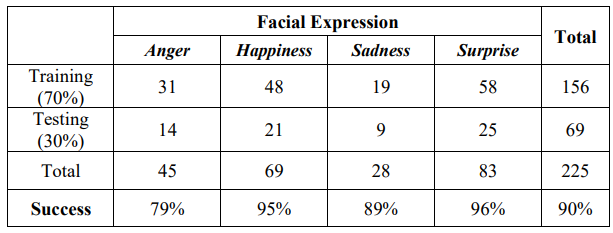
\includegraphics[width=10cm]{Images/rf_result.png}
    \caption{Random Forest Classification Accuracy} \footnotesize{Table from \cite{munasinghe_2018_facial}}
    \label{fig:rf_result}
\end{figure}
\\
\indent According to Munasinghe (2018), \gls{rf} Classifier are capable of handling facial expression variability well and without overfitting.
Also, the researcher asserts that facial landmarks (Figure \ref{fig:facial_landmark}) provide an accurate feature extraction capability that capture subtle changes in facial emotions.
A facial feature vector obtained from these landmarks and normalized to reduce variance in face size is used to discern emotions with a \gls{rf} Classifier.
With the aid of feature vector, the \gls{rf} Classifier achieved an average success rate of 90\% in classifying four different emotions: anger, happiness, sadness, and surprise (Figure \ref{fig:rf_result}).
\\
\begin{figure}[!ht]
    \centering
    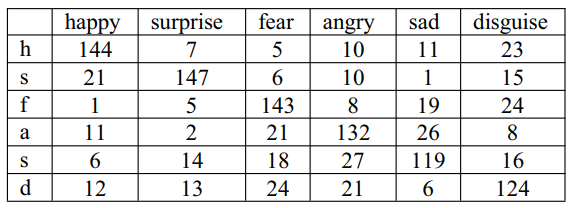
\includegraphics[width=10cm]{Images/svm_result.png}
    \caption{Support Vector Machine Accuracy} \footnotesize{Table from \cite{xia_2014_facial}}
    \label{fig:svm_result}
\end{figure}
\\
\indent Li Xia (2014) presents a unique method of facial emotion detection that employs multi-classification \gls{svm}.
The study proposes a two-on-two classification method which is an innovative approach to overcome the limitations of traditional classification methods like one-against-one (classifier is trained for each pair of classes) and one-against-the-rest (classifier is trained against all other classes combined).
With this novel method, the classification process is faster with fewer sub-classifiers and reduced classification errors.
The results of this study were impressive, showing the classifier in this investigation demonstrated a high average recognition rate of 92.7\% when six distinct emotions were considered, including happiness, surprise, anger, fear, disgust, and sadness. 
\\
\section{Music Recommendation based on FER}
From Chakrapani et al.'s approach, music recommendation system with deep learning algorithm could enhance the listening experience by accurately detect and interpret the user's emotions.
This is achieved by using \gls{cnns} to analyze the user's age, gender, and facial emotion. Based on these data, the system would cater to the user's preferences and present mood.
To ascertain the user's emotional state, they used the webcam to take pictures of the user and then processed the image using the \gls{cnns} models.
The system then provided tailored music recommendations based on the predictions generated by the \gls{cnns} models. 
This approach offers a creative and user-centric alternative for music selection based on emotional cues while streamlining playlist construction and management.\cite{mrchakrapanids_2023_music}
\\
\indent Additionally, Athavle et al. discovered that using \gls{cnns} model helps a music recommendation system to accurately detect emotions and subsequently recommend music that aligns with the user's mood.
They train a \gls{cnns} model for emotion detection in their work. 
While maintaining great precision, this method lowers total system costs and computing time.
The system uses real-time emotion detection to work, and then sends the data to the \gls{cnns} model to classify the user's emotions. 
An appropriate playlist will be recommended as soon as the technology determines the user's current feeling, making the user experience engaging and responsive.
In order to guarantee optimal classification accuracy and efficacy, they employed categorial cross-entropy as a loss function to manage missing and anomalous values inside the FER2013 dataset.
Despite their result being less accurate than Chakrapani et al.'s work (71\%), it nevertheless shows that the model is effective and trustworthy in identifying emotions from facial expressions. \cite{athavle_2021_music}
 % Section/Chapter entries can be done in the Main.tex file or in a  
                       % separate tex file for longer and more complex documents

% -------------------  REQUIREMENTS  ---------------------
\chapter{Requirements}
\section{Functional Requirements and Non-functional Requirements}
\subsection{Functional Requirements}
\begin{longtable}{ |m{1cm}|m{3.5cm}|m{7cm}|m{1.5cm}| }
    \hline
    \textbf{Req. No.} & \textbf{Categories} & \textbf{Requirements} & \textbf{Priority} \\
    \hline
    \endfirsthead

    \hline
    \textbf{Req. No.} & \textbf{Categories} & \textbf{Requirements} & \textbf{Priority} \\
    \hline
    \endhead
    FR1 & \multirow{5}{=}{User Registration and Account Management} & The system must allow user to register by providing a unique username, user's actual name, date of birth, email, and password. & High \\
    \cline{1-1} \cline{3-4}
    FR2 &  & The system must verify user accounts through an email verification process. & High \\
    \cline{1-1} \cline{3-4}
    FR3 &  & Users must be able to login with their email or username and password. A "Remember Me" option should allow users to stay logged in for 7 days. & High \\
    \cline{1-1} \cline{3-4}
    FR4 &  & Users can access a settings page to update their name, date of birth, email, password, and profile picture. Usernames cannot be changed. & Medium \\
    \cline{1-1} \cline{3-4}
    FR5 &  & Users must be able to reset their passwords through a password reset feature on the login page. & Medium \\
    \hline
    FR6 & Facial Emotion Recognition & The application integrates a machine learning model to recognize user's facial emotions via their device's camera. & High \\
    \hline
    FR7 & \multirow{2}{=}{Spotify Web Playback Integration} & The system integrates with Spotify Web Playback SDK to play music within the web application. & High \\
    \cline{1-1} \cline{3-4}
    FR8 &  & The application must allow users to connect their Spotify account before accessing music playback services. This integration should facilitate authentication and authorization seamlessly within the web application. & High \\
    \hline
    FR9 & Music Recommendation System & The application must generate playlists based on the user's recognized emotion using an algorithm. & High \\
    \hline
    FR10 & \multirow{2}{=}{User Interface and Experience} & The web application supports a toggle between light and dark themes, automatically detecting and applying the user's device theme upon first use. & Medium \\
    \cline{1-1} \cline{3-4}
    FR11 &  & The application supports multiple languages: English, Japanese, Chinese, Korean, and Malay. & Low \\
    \hline
\end{longtable}
\pagebreak
\subsection{Non-Functional Requirements}
\begin{longtable}{ |m{1.5cm}|m{3.5cm}|m{7cm}|m{1.5cm}| }
    \hline
    \textbf{Req. No.} & \textbf{Categories} & \textbf{Requirements} & \textbf{Priority} \\
    \hline
    \endfirsthead

    \hline
    \textbf{Req. No.} & \textbf{Categories} & \textbf{Requirements} & \textbf{Priority} \\
    \hline
    \endhead
    NFR1 & \multirow{2}{=}{Performance and Scalability} & The application shall load within 3 seconds for 95\% of its users under standard network conditions. & High \\
    \cline{1-1} \cline{3-4}
    NFR2 &  & The system must be scalable to support up to 100 concurrent users without significant degradation in performance. & High \\
    \hline
    NFR3 & \multirow{5}{=}{Compliance and Security} & All user data, including passwords and personal information, must be encrypted. & High \\
    \cline{1-1} \cline{3-4}
    NFR4 &  & The application must implement secure authentication mechanisms to prevent unauthorized access. & High \\
    \cline{1-1} \cline{3-4}
    NFR5 &  & User data must be stored in a secure database with access strictly limited ot the backend server. The database shall not be directly accessible from any public network (0.0.0.0/0). & High \\
    \cline{1-1} \cline{3-4}
    NFR6 &  & User passwords must be encrypted using a secure hashing algorithm (e.g., bcrypt) to ensure their safety even in the event of a data breach. & High \\
    \cline{1-1} \cline{3-4}
    NFR7 &  & All forms of data transmission involved in user authentication and registration must be over HTTPS, and sensitive information shall not appear in URLs or any part of the HTTP request visible to the client side. & High \\
    \cline{1-1} \cline{3-4}
    NFR8 &  & The application must comply with relevant data protection and privacy regulations, including GDPR where applicable, ensuring user's rights to privacy and data security are upheld. & High \\
    \hline
    NFR9 & \multirow{2}{=}{Usability} & The application shall be designed with a user-friendly interface, ensuring ease of navigation and accessibility. & Medium \\
    \cline{1-1} \cline{3-4}
    NFR10 &  & User input fields should provide immediate feedback to correct errors or invalid data. & Medium \\
    \hline
    NFR11 & \multirow{2}{=}{Compatibility and Interoperability} & The web application must be compatible with the latest versions of Chrome, Firefox, Safari and Edge browsers. & High \\
    \cline{1-1} \cline{3-4}
    NFR12 &  & The system must ensure seamless integration with the Spotify API and maintain compatibility with Spotify's update. & High \\
    \hline
    NFR13 & \multirow{2}{=}{Localization and Internationalization} & The application must support multi-language interfaces, allowing users to switch languages easily. & Medium \\
    \cline{1-1} \cline{3-4}
    NFR14 &  & Date and time formats should adapt to the user's selected language and region preferences. & Low \\
    \hline
    NFR15 & \multirow{2}{=}{Maintenance and Support} & The system should be designed to allow easy updates and maintenance without significant downtime. & Medium \\
    \cline{1-1} \cline{3-4}
    NFR16 &  & Documentation must be provided for end-users and developers, detailing usage, integration features, and troubleshooting steps. & Medium \\
    \hline
    NFR17 & \multirow{3}{=}{Application Performance} & The facial emotion recognition feature must provide a response within 5 seconds from the time of user's request under standard network conditions. & High \\
    \cline{1-1} \cline{3-4}
    NFR18 &  & The system should ensure a Spotify playback start time of less than 3 seconds after user selection or playlist generation. & High \\
    \cline{1-1} \cline{3-4}
    NFR19 &  & The web application's overall time to interactive (TTI) should not exceed 5 seconds for 90\% of its users under standard network conditions. & High \\
    \hline
    NFR20 & \multirow{2}{=}{User Interface Design} & The application must adhere to WCAG 2.1 AA standards for color contrast, navigability, and text size to ensure accessibility for users with disabilities. & High \\
    \cline{1-1} \cline{3-4}
    NFR21 &  & All user interface components (buttons, links, form elements) must be navigable using a keyboard in a logical order to support users with mobility or visual impairments. & High \\
    \hline
    NFR22 & \multirow{2}{=}{Data Handling and Authentication} & Implement OAuth 2.0 for secure authentication with Spotify, ensuring that user credentials are handled safety and in line with best security practices. & High \\
    \cline{1-1} \cline{3-4}
    NFR23 &  & Apply secure session management practices, including the generation of unique session tokens for users during login and their secure storage on the client side. & High \\
    \hline
\end{longtable}

\section{Requirements Specification}
\subsection{Use Cases and UML Diagrams}

 % Section/Chapter entries can be done in the Main.tex file or in a  
                       % separate tex file for longer and more complex documents

% -------------------  METHODOLOGY  ---------------------
\chapter{Methodology}
\section{Introduction}
To effectively navigate the intricacies of software development and guarantee the project's success, choosing an appropriate approach is essential.
The concepts, procedures, and practices that guide a project's development, implementation, and completion are collectively referred to methodology.
The variety of alternative methods, each with specific advantages and applicability to various project types, means that selecting a methodology should be done with careful consideration.
This section explores the reasoning behind the choice of an Agile-based methodology, with a particular emphasis on the Kanban methodology, made by the use of Notion application for project management.
This decision was driven by the project's requirement for flexibility, continuous improvement, and a visual workflow management system. 
The following sections will outline the comparative comparison between various approaches, along with the reasoning behind choosing Agile due to its alignment with the project's objectives and task specifications.
\\
\section{Research Methodology}
\subsection{Waterfall methodology}
Waterfall methodology, with its linear and sequential approach, stands as a traditional yet relevant framework for software development projects that require a clear, phased progression.
Requirements, design, implementation, testing, development and maintenance are the steps in this process.
They guarantee that one phase must be finished before moving on to the next, which makes them especially appropriate for projects with stable, well-defined requirements that are unlikely to change.
Crespo-Santiago \& de la Cruz Dávila-Cosme (\citeyear{cresposantiago_2022_waterfall}) highlight the Waterfall methodology helps maintain the scope of their library project within the requirements, estabilishing cost and time control, and documenting evidence of project governance.
\begin{figure}[H]
    \centering
    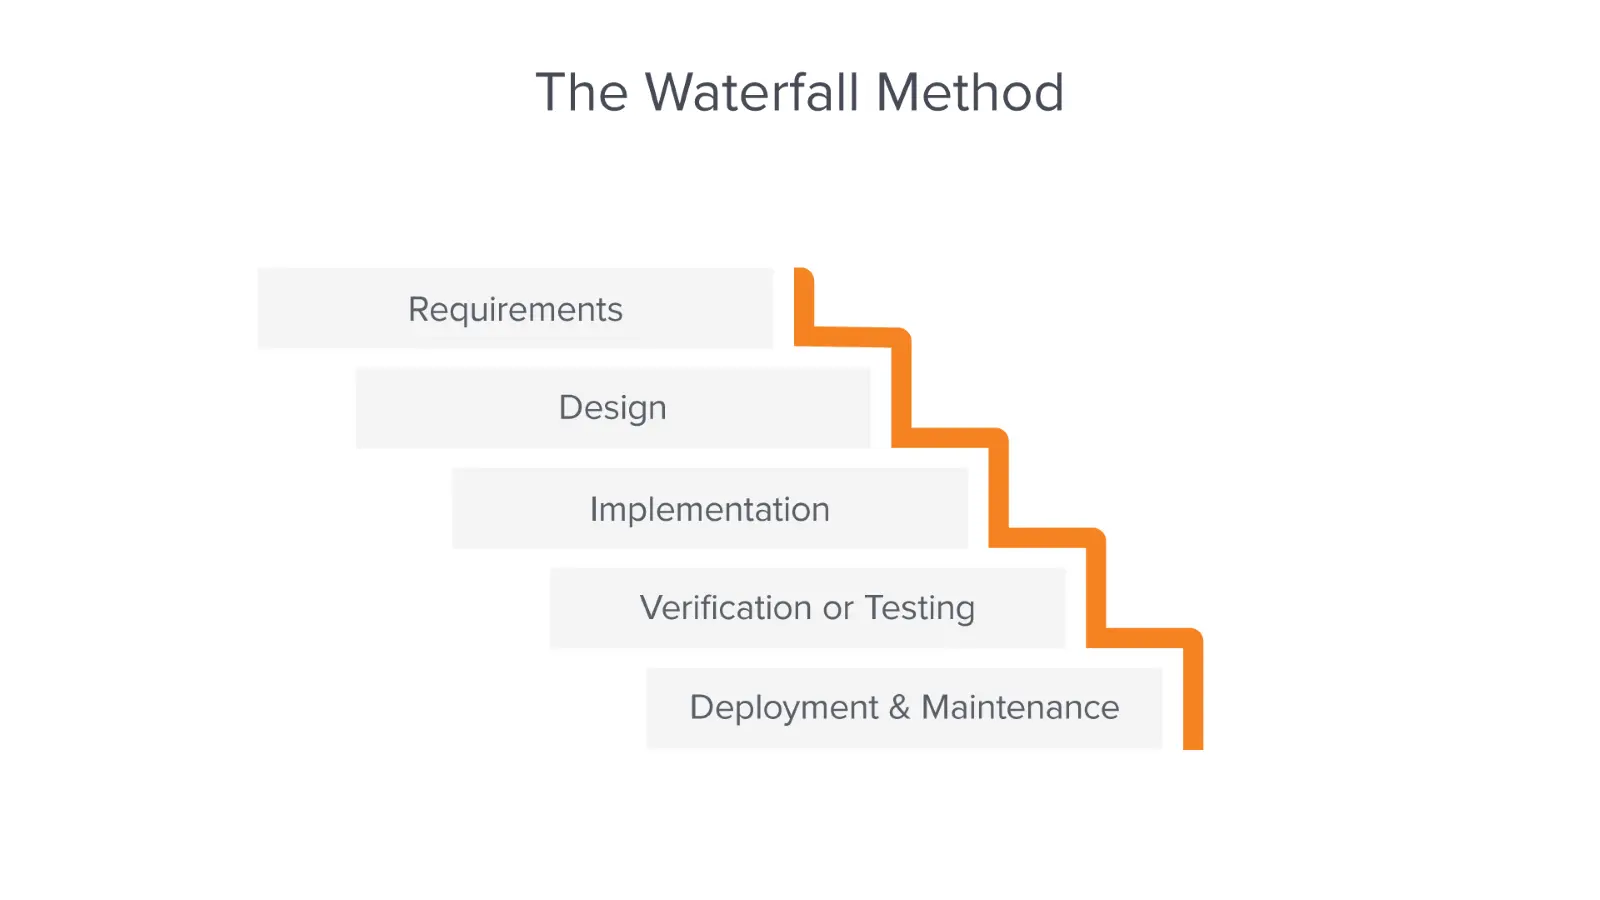
\includegraphics[width=10cm]{Images/watefall.png}
    \caption{Waterfall Methodology \citep{communitcationteam_2022_waterfall}}
    \label{fig:waterfall}
\end{figure}

\subsection{Spiral methodology}
\begin{figure}[H]
    \centering
    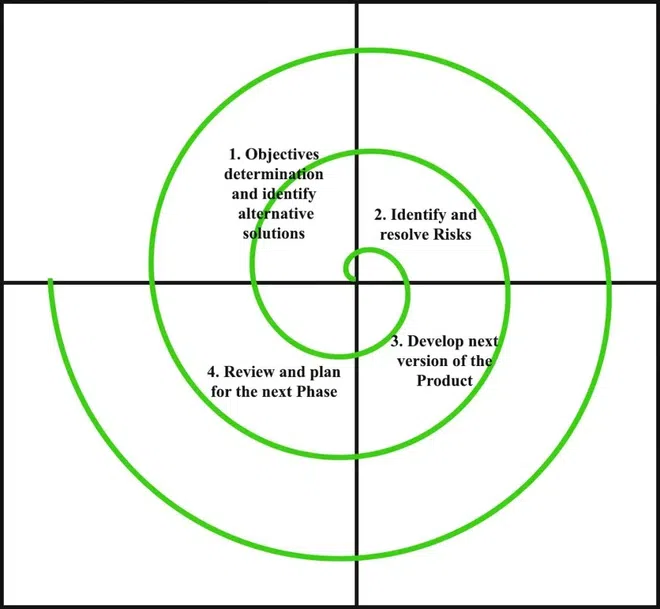
\includegraphics[width=7cm]{Images/spiral.png}
    \caption{Spiral Methodology \citep{kumarpal_2018_software}}
    \label{fig:spiral}
\end{figure}
Spiral methodology, an evolutionary software development process introduced by Barry Boehm in 1986, is a model for process flexibility and risk control in software development \citep{boehm_1986_a}.
The methodology is distinguished by its four-phase cycle approach, which includes planning, risk analysis, implementation, evaluation.
This allows for ongoing iterations that involve setting project goals, identifying potential risks, carrying out development, and incorporating stakeholder feedback.
Its iterative design ensures a flexible and adaptive development process by permitting incremental product improvements based on changing needs and stakeholder input.
The Spiral methodology provides a methodical approach to managing the complexities and uncertainties inherent in software development. 
It shines in contexts where project needs are ambiguous or subject to change because of its heavy emphasis on risk management. 

\subsection{Agile methodology}
\begin{figure}[H]
    \centering
    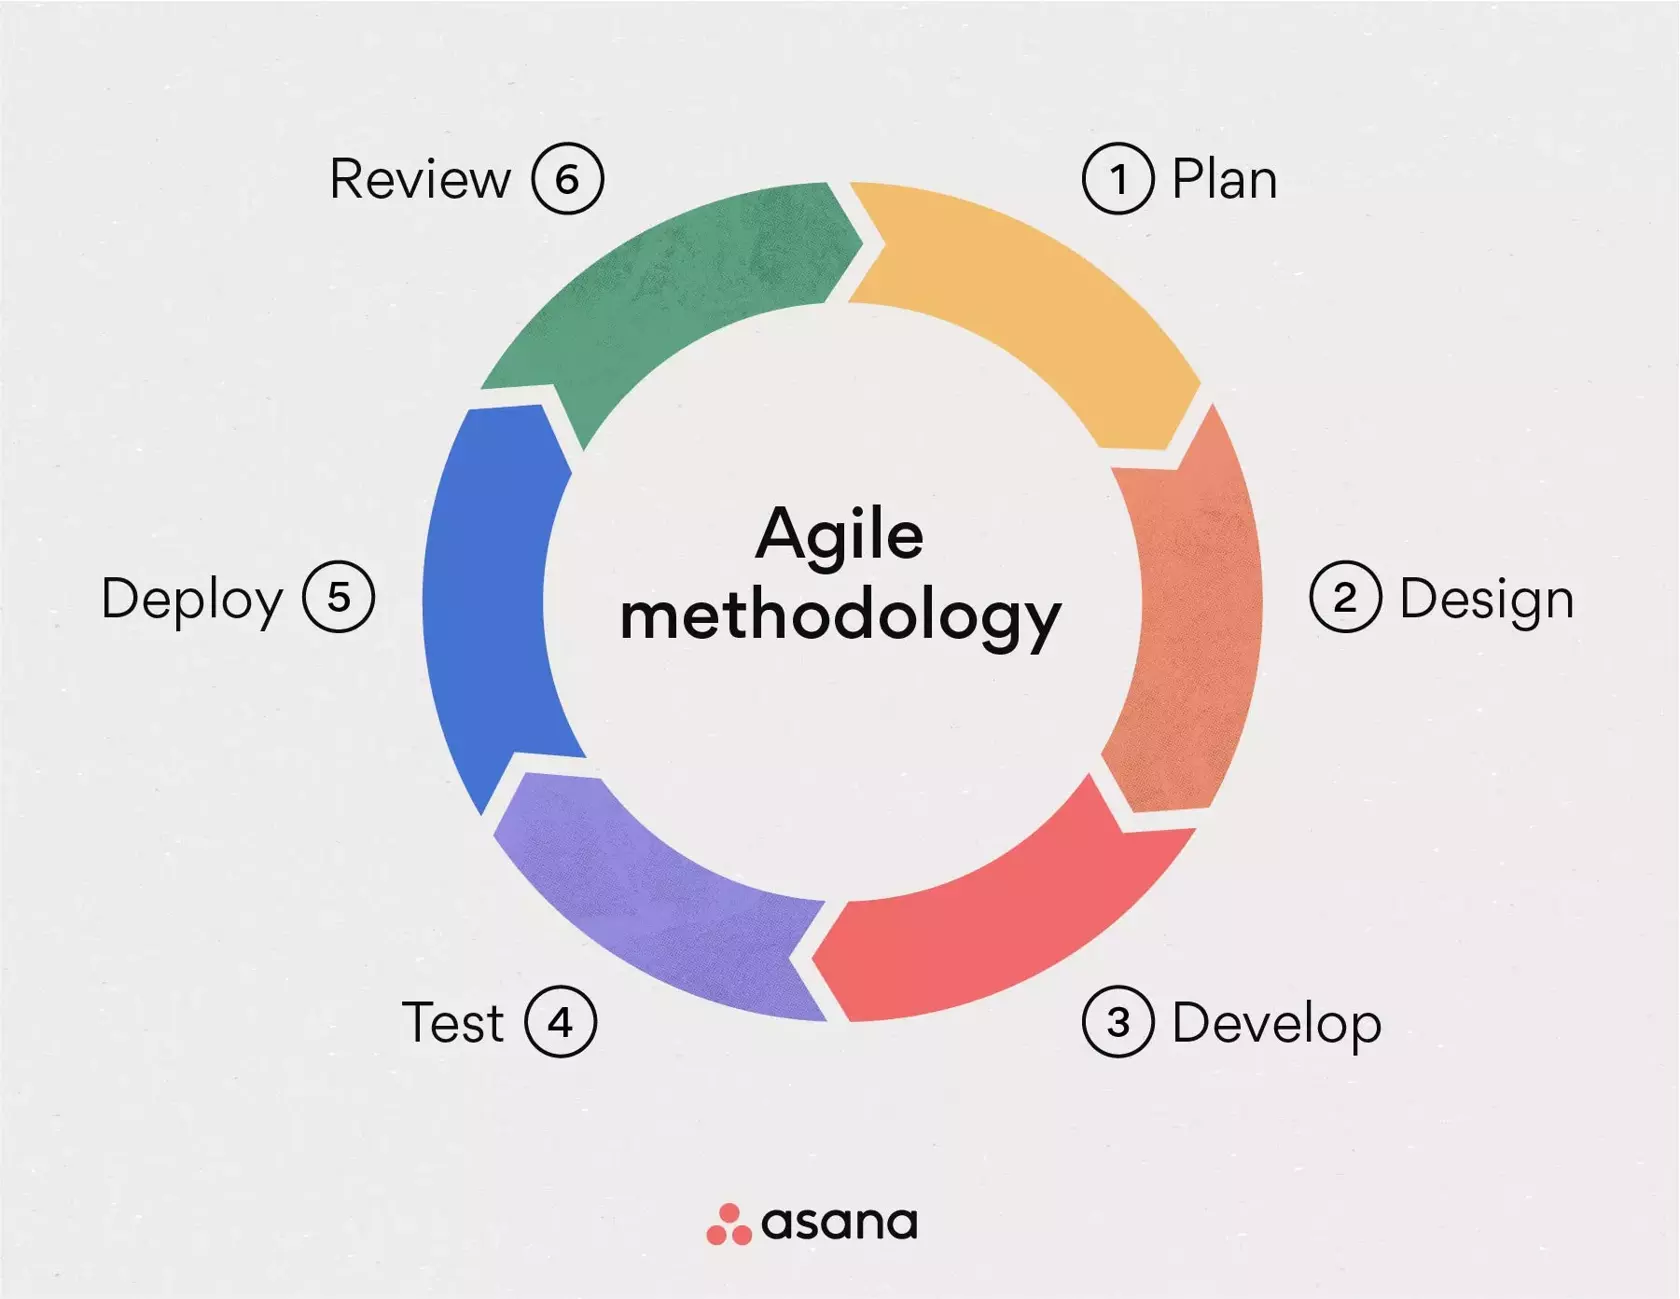
\includegraphics[width=7cm]{Images/agile.png}
    \caption{Agile Methodology \citep{laoyan_2022_what}}
    \label{fig:agile}
\end{figure}
Agile methodology, an approach originated from the Agile Manifesto, published in 2001 by a group of software developers, prioritizes adaptability, collaboration, customer satisfaction and timely delivery of high-quality software \citep{laoyan_2022_what}.
While implementing Agile methodology, project is breaks into small, manageable pieces, known as iterations or sprints.
Each sprint involves cross-functional teams working on various aspects like planning, design, coding, and testing, with a working iteration of the product delivered at the end of each cycle. 
This methodology works effectively for projects whose requirements are changing or unclear since it allows ongoing feedback and adjustment. 

\section{Comparison and Selection}
Software development can be approached differently using the Agile, Waterfall, and Spiral techniques, each with its own set of benefits and difficulties.
As detailed in Table \ref{tab:methodologies}, Agile is highly flexible and adaptable, ideal for projects with evolving requirements, but may lead to unpredictable costs.
Waterfall is straightforward and orderly, perfect for projects with well-defined requirements, but inflexible to changes.
Spiral combines iterative development with focusing on risk management, but it could be costly. 
\newpage
The project's scale and the clarity of its needs determine which technique is best: Waterfall for its structure, Agile for its flexibility, or Spiral for its risk emphasis.
\begin{table}[H]
    \caption{Comparison of Methodologies}
    \centering
    \begin{tabularx}{\textwidth}{>{\bfseries}lXXX}
    \toprule
    Aspect & Agile & Waterfall & Spiral \\
    \addlinespace
    Pros & 
    \begin{itemize}[leftmargin=*, nosep, after=\strut]
        \item High flexibility and adaptability to changes.
        \item Frequent releases and feedback.
        \item Enhanced customer satisfaction.
        \item Reduced time to market.
    \end{itemize} & 
    \begin{itemize}[leftmargin=*, nosep, after=\strut]
        \item Simple and easy to understand and use.
        \item Clear project milestones and deliverables.
        \item Well-suited for projects with defined requirements.
    \end{itemize} & 
    \begin{itemize}[leftmargin=*, nosep, after=\strut]
        \item Focus on risk management.
        \item Flexibility in design and development.
        \item Suitable for large, complex projects with uncertain risks.
    \end{itemize} \\
    \addlinespace
    Cons & 
    \begin{itemize}[leftmargin=*, nosep, after=\strut]
        \item Less predictable budget and timeline.
        \item Requires close collaboration and customer involvement.
        \item Not ideal for low-change projects or those with fixed requirements.
    \end{itemize} & 
    \begin{itemize}[leftmargin=*, nosep, after=\strut]
        \item Difficult to incorporate changes once the project has started.
        \item Potential for late discovery of problems or errors.
        \item Not suitable for projects where requirements may evolve.
    \end{itemize} & 
    \begin{itemize}[leftmargin=*, nosep, after=\strut]
        \item Can be complex and costly to implement.
        \item Requires significant risk assessment expertise.
        \item May lead to prolonged project duration due to iterative nature.
    \end{itemize} \\
    \bottomrule
    \end{tabularx}
    \label{tab:methodologies}
\end{table}  

\section{Justification for Choosing Agile}
The Agile methodology, particularly the Kanban variant, was chosen in order to satisfy the demand for an adaptable, graphical, and iterative developments process.
Given the dynamic nature of the project and its ever-changing objectives, Kanban, which places a strong focus on continuous delivery and workflow efficiency, is an excellent fit.
\begin{figure}[H]
    \centering
    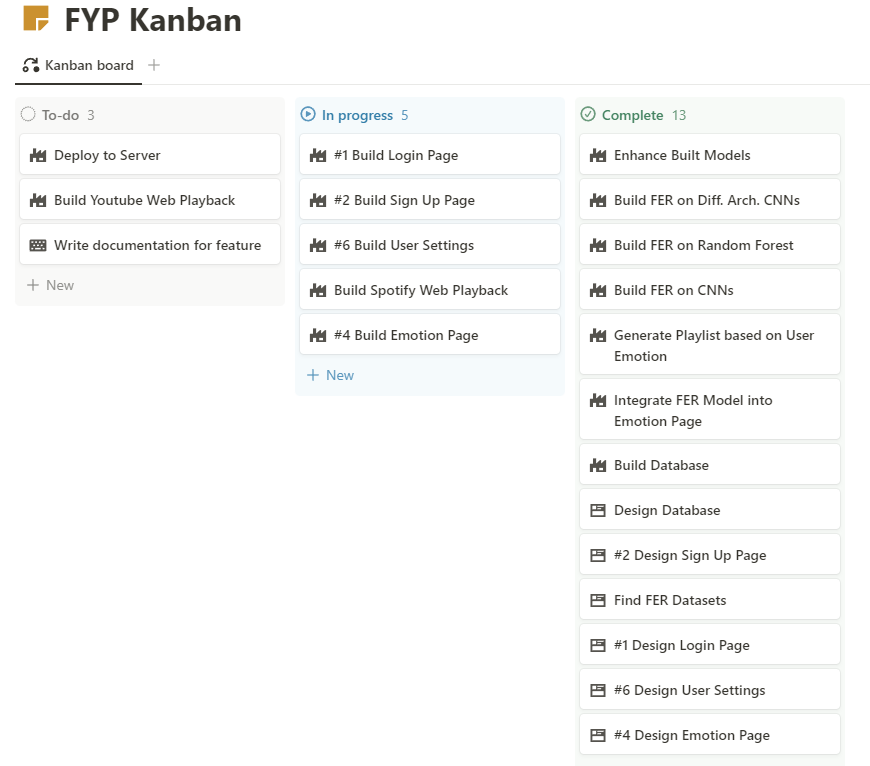
\includegraphics[width=12cm]{Images/kanban.png}
    \caption{Kanban from Notion}
    \label{fig:kanban}
\end{figure}
\indent In this project, Kanban is implementing using Notion.
It gives tasks a visual representation, making it easier to organize and keep track of them as they go through various stages of development.
Also, with the adaptability of Notion's platform, project plans could be updated easily which is crucial for keeping the plan responsive to changing project dynamics.
\\
\indent Kanban method's inherent simplicity and its focus on delivering work just-in-time are particularly beneficial for projects demanding flexibility and time efficiency.
Kanban with Notion provides a clear picture of the project's progress, enabling developer to identify and resolve bottlenecks quickly, and efficiently manage task prioritization.
Therefore, the combination of Notion's features with Agile Kanban creates a strong foundation for project management by fusing Kanban's visual clarity and streamlined efficiency with Agile's flexibility. 
Lastly, Gantt chart (See Figure~\ref{fig:gantt-chart}) is also used in this project to keep track on the progress.
 % Section/Chapter entries can be done in the Main.tex file or in a  
                       % separate tex file for longer and more complex documents

% -------------------  DESIGN  ---------------------
\chapter{Design}
\section{Introduction}
The design phase of the web application, focused on using emotion recognition to generate music therapy playlists, represents a bridge from theoretical concepts to a operational system.
The varied design approaches that were used to develop an application with a solid technical framework and user-friendly interface are covered in this section.
\\
\indent The core aspect of the application is how it uses captured frame analysis to determine a user's emotional state by utilizing \gls{fer} technology.
This sense of emotional then guided the creation of customized music playlists, fusing the advanced machine learning techniques with the restorative properties of music to provide a unique advantageous user experience.
\\
\indent This project uses diagrams such as block diagram, use case diagram, sequence diagram and etc., where each focusing on a different aspect of the architecture and functionality of the system.
Futhermore, this section delves into the visual and functional components of the application's user interface as illustrated by the Logo Design and Interface Design.
The logo, as the visual cornerstone of the application's brand identify, have been thoughtfully designed to improve application usability and user engagement.
\\
\indent Additionally, the \gls{ml} model architecture design, which describes the underlying algorithms and data processing methods used in \gls{fer}, is also discussed in this section.
This discussion covers the model's validation, training, and integration into the broader application ecosystem to ensure accurate emotional analysis.
\\
\indent All of these components provide a thorough explanation of the system's design, addressing structural, behavioral, and aesthetic factors from the abstract to the concrete.

\section{Web Application}
This section explores the design decisions made for the web application's architecture and aesthetics.
It describes how the architecture of the system was designed to optimize usability and functionality, ensuring seamless integration of the \gls{fer} technology with the music recommendation system.
\\
\subsection{UML Diagrams}
\subsubsection{Block Diagram}
Block diagram present a high-level overview of the system's architecture, highlighting the major components and their interactions \citep{freeman_block}.
This offers insights into the overall system design and its flow.
\begin{figure}[H]
    \centering
    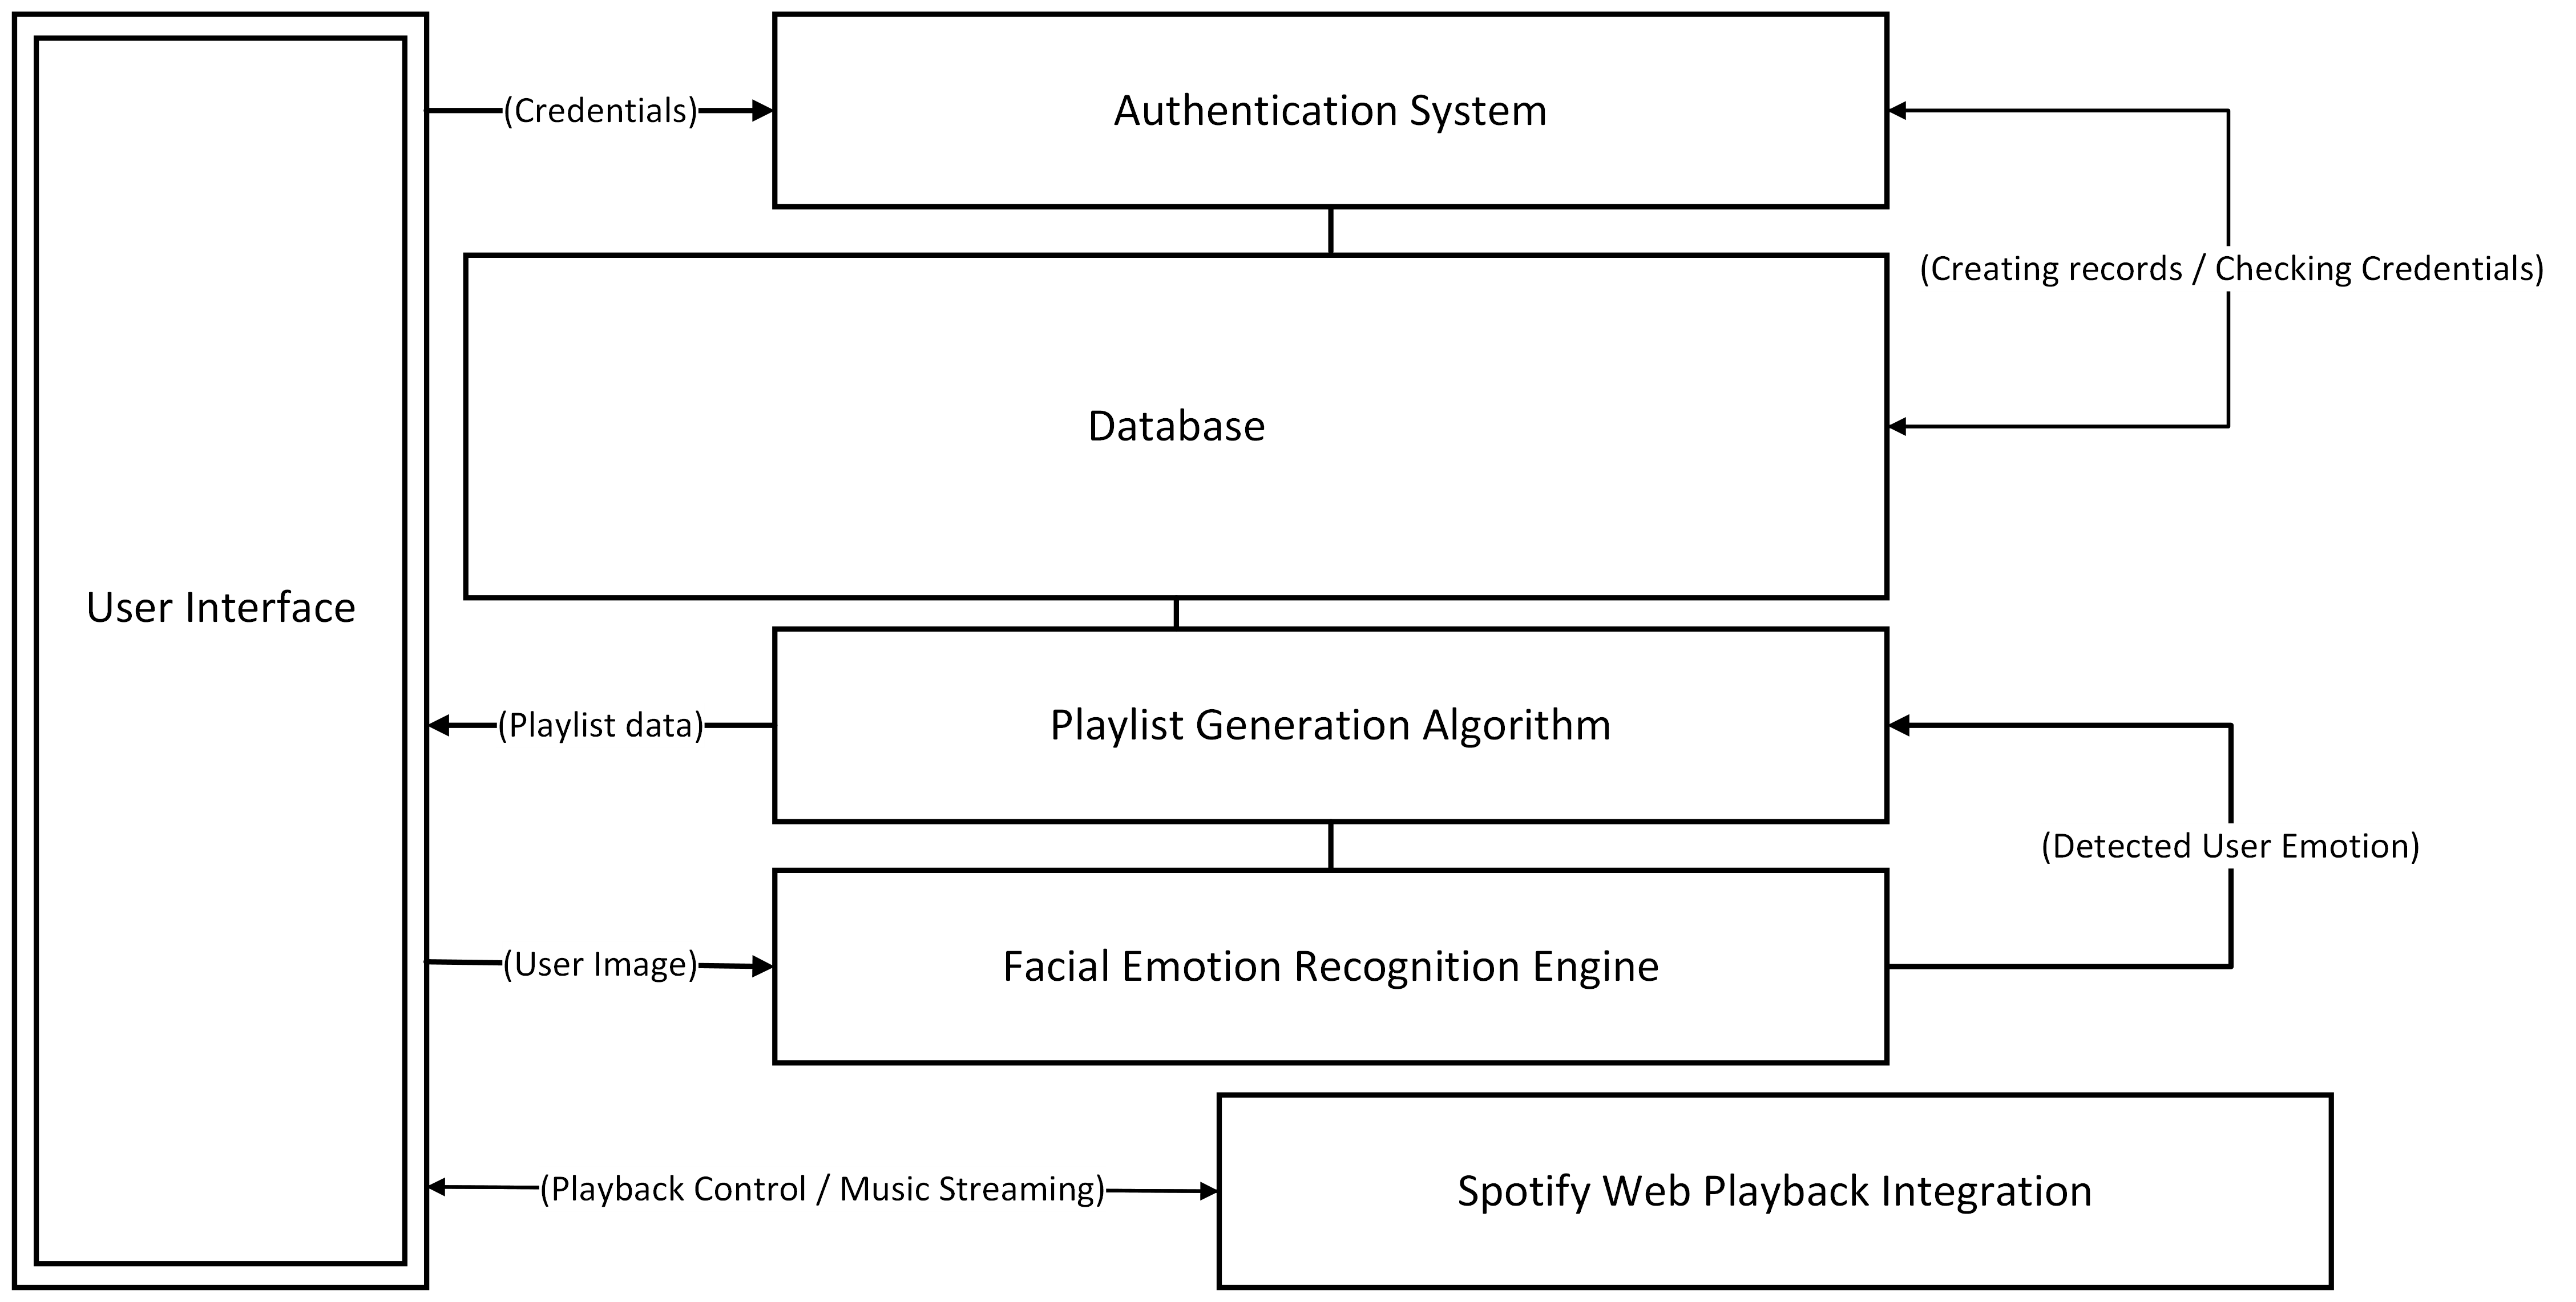
\includegraphics[width=15cm]{Images/block.png}
    \caption{Block Diagram}
    \label{fig:block}
\end{figure}
\indent As shown in Figure \ref{fig:block}, there are different components and each component has its own responsibilities to enable \gls{fer} and playlist generation for music therapy.
\gls{ui} is the gateway through which users interact with the application.
It captures user inputs such as credentials for the authentication process, frames for emotion recognition, and user actions for music playback controls.

\newpage

\indent Authentication System manages user identity verification and access control.
When user provides credentials, either username or email, and password to this component, it will validates them against stored data in the database. 
Upon successful validation, users can access the full functionality of the services.
This component also handles account creation, where new user details are stored securely in the database.
\\
\indent Database stores and manages all persistent data, including user credentials, profile information, and any data pertinent to playlist generation processes.
It ensures data integrity and provides efficient access for other components.
\gls{fer} Engine utilizes advanced algorithms and machine learning models.
This engine analyses captured frame, which contains user's facial expression, to detect emotional states.
The result of this analysis is then used to tailor the music playlist to the user's current emotional needs.
\\
\indent Playlist Generation Algorithm takes the detected emotion from the \gls{fer} Engine and constructs a playlist that suits the identified mood and therapeutic requirements.
It queries a database of songs, which stored internally, to select appropriate tracks.
Then, Spotify Web Playback Integration acts as the music service interface. 
This component is responsible for fetching the actual music tracks from Spotify and controlling the playback within the application, such as playing, pausing, and etc. based on user input through the \gls{ui}.
\\
\indent This diagram simplifies the conceptual understanding of the system and forms the architectural backbone of the application.
It also outlines how user actions translate into system responses and result in a music therapy experience.
\\
\subsubsection{Use Case Diagram}
Use Case diagram is a visual representation of the system's functionalities and the interactions that different types of users have with these functionalities \citep{ibm_2021_usecase}.
\begin{figure}[H]
    \centering
    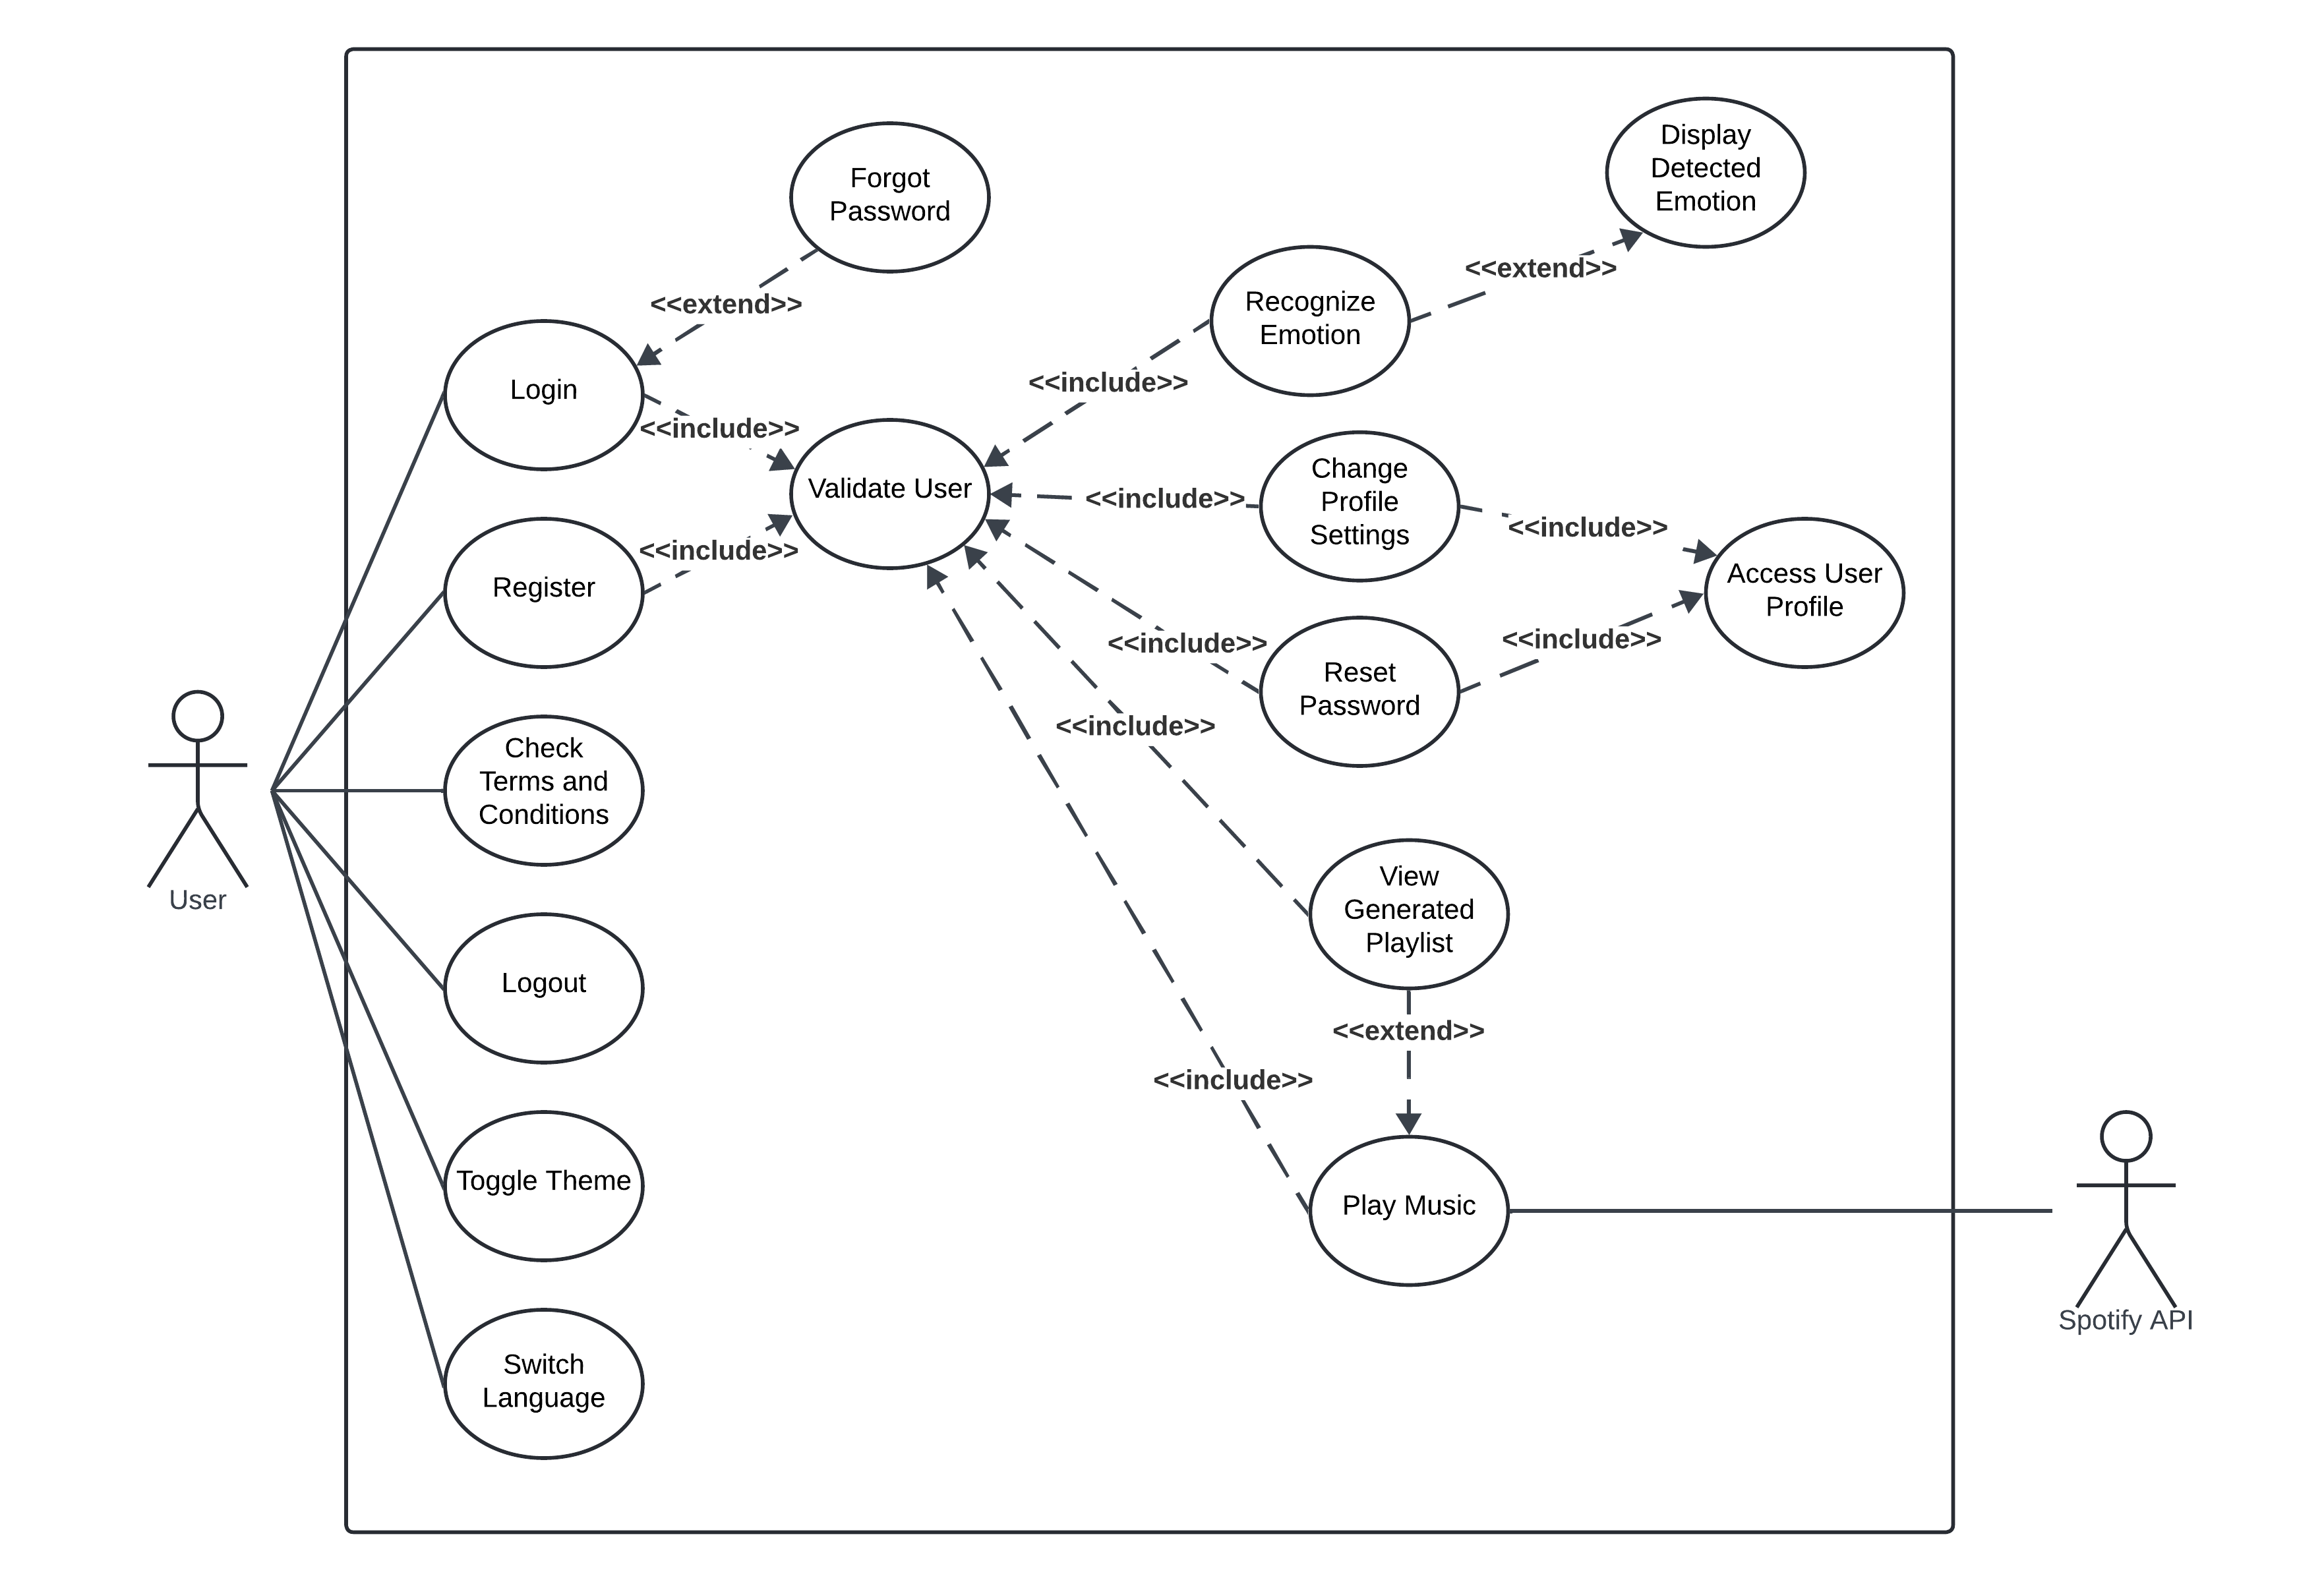
\includegraphics[width=16cm]{Images/usecase.png}
    \caption{Use Case Diagram}
    \label{fig:usecase}
\end{figure}
\indent As shown in Figure \ref{fig:usecase}, there are two actors, `User' and the `Spotify API'.
The `User' represents any individual who interacts with the application for its services.
The `Spotify API' acts as an external system that the application communicates with to stream music.
\\
\indent The use case diagram delineates the extent of the application's capability from the `User' point of view by illustrating the user interactions.
This helps to understand what the system does, but not how it does it, thus separating the `what' from the `how' in system functionalities.
When a use case incorporates another's behavior or expands the behavior under some circumstances, it is represented by dashed lines with arrows labelled `includes' and `extends.'
For example, several use cases in the application such as `Recognize Emotion', `Change Profile Settings', and `Play Music', require the `User' to be authenticated.
This precondition is captured in the `Validate User' use case, which is included in these use cases to ensure that the `User' is logged in before granting access to the services.
\\
\subsubsection{Sequence Diagrams}
Sequence diagrams provide an illustrative view of how various components of a system work together ot accomplish a process, acting as blueprints of interaction across time \citep{bell_2004_explore}.
They are especially helpful in understanding the flow of messages and actions between objects in response to software system events.
\begin{figure}[H]
    \centering
    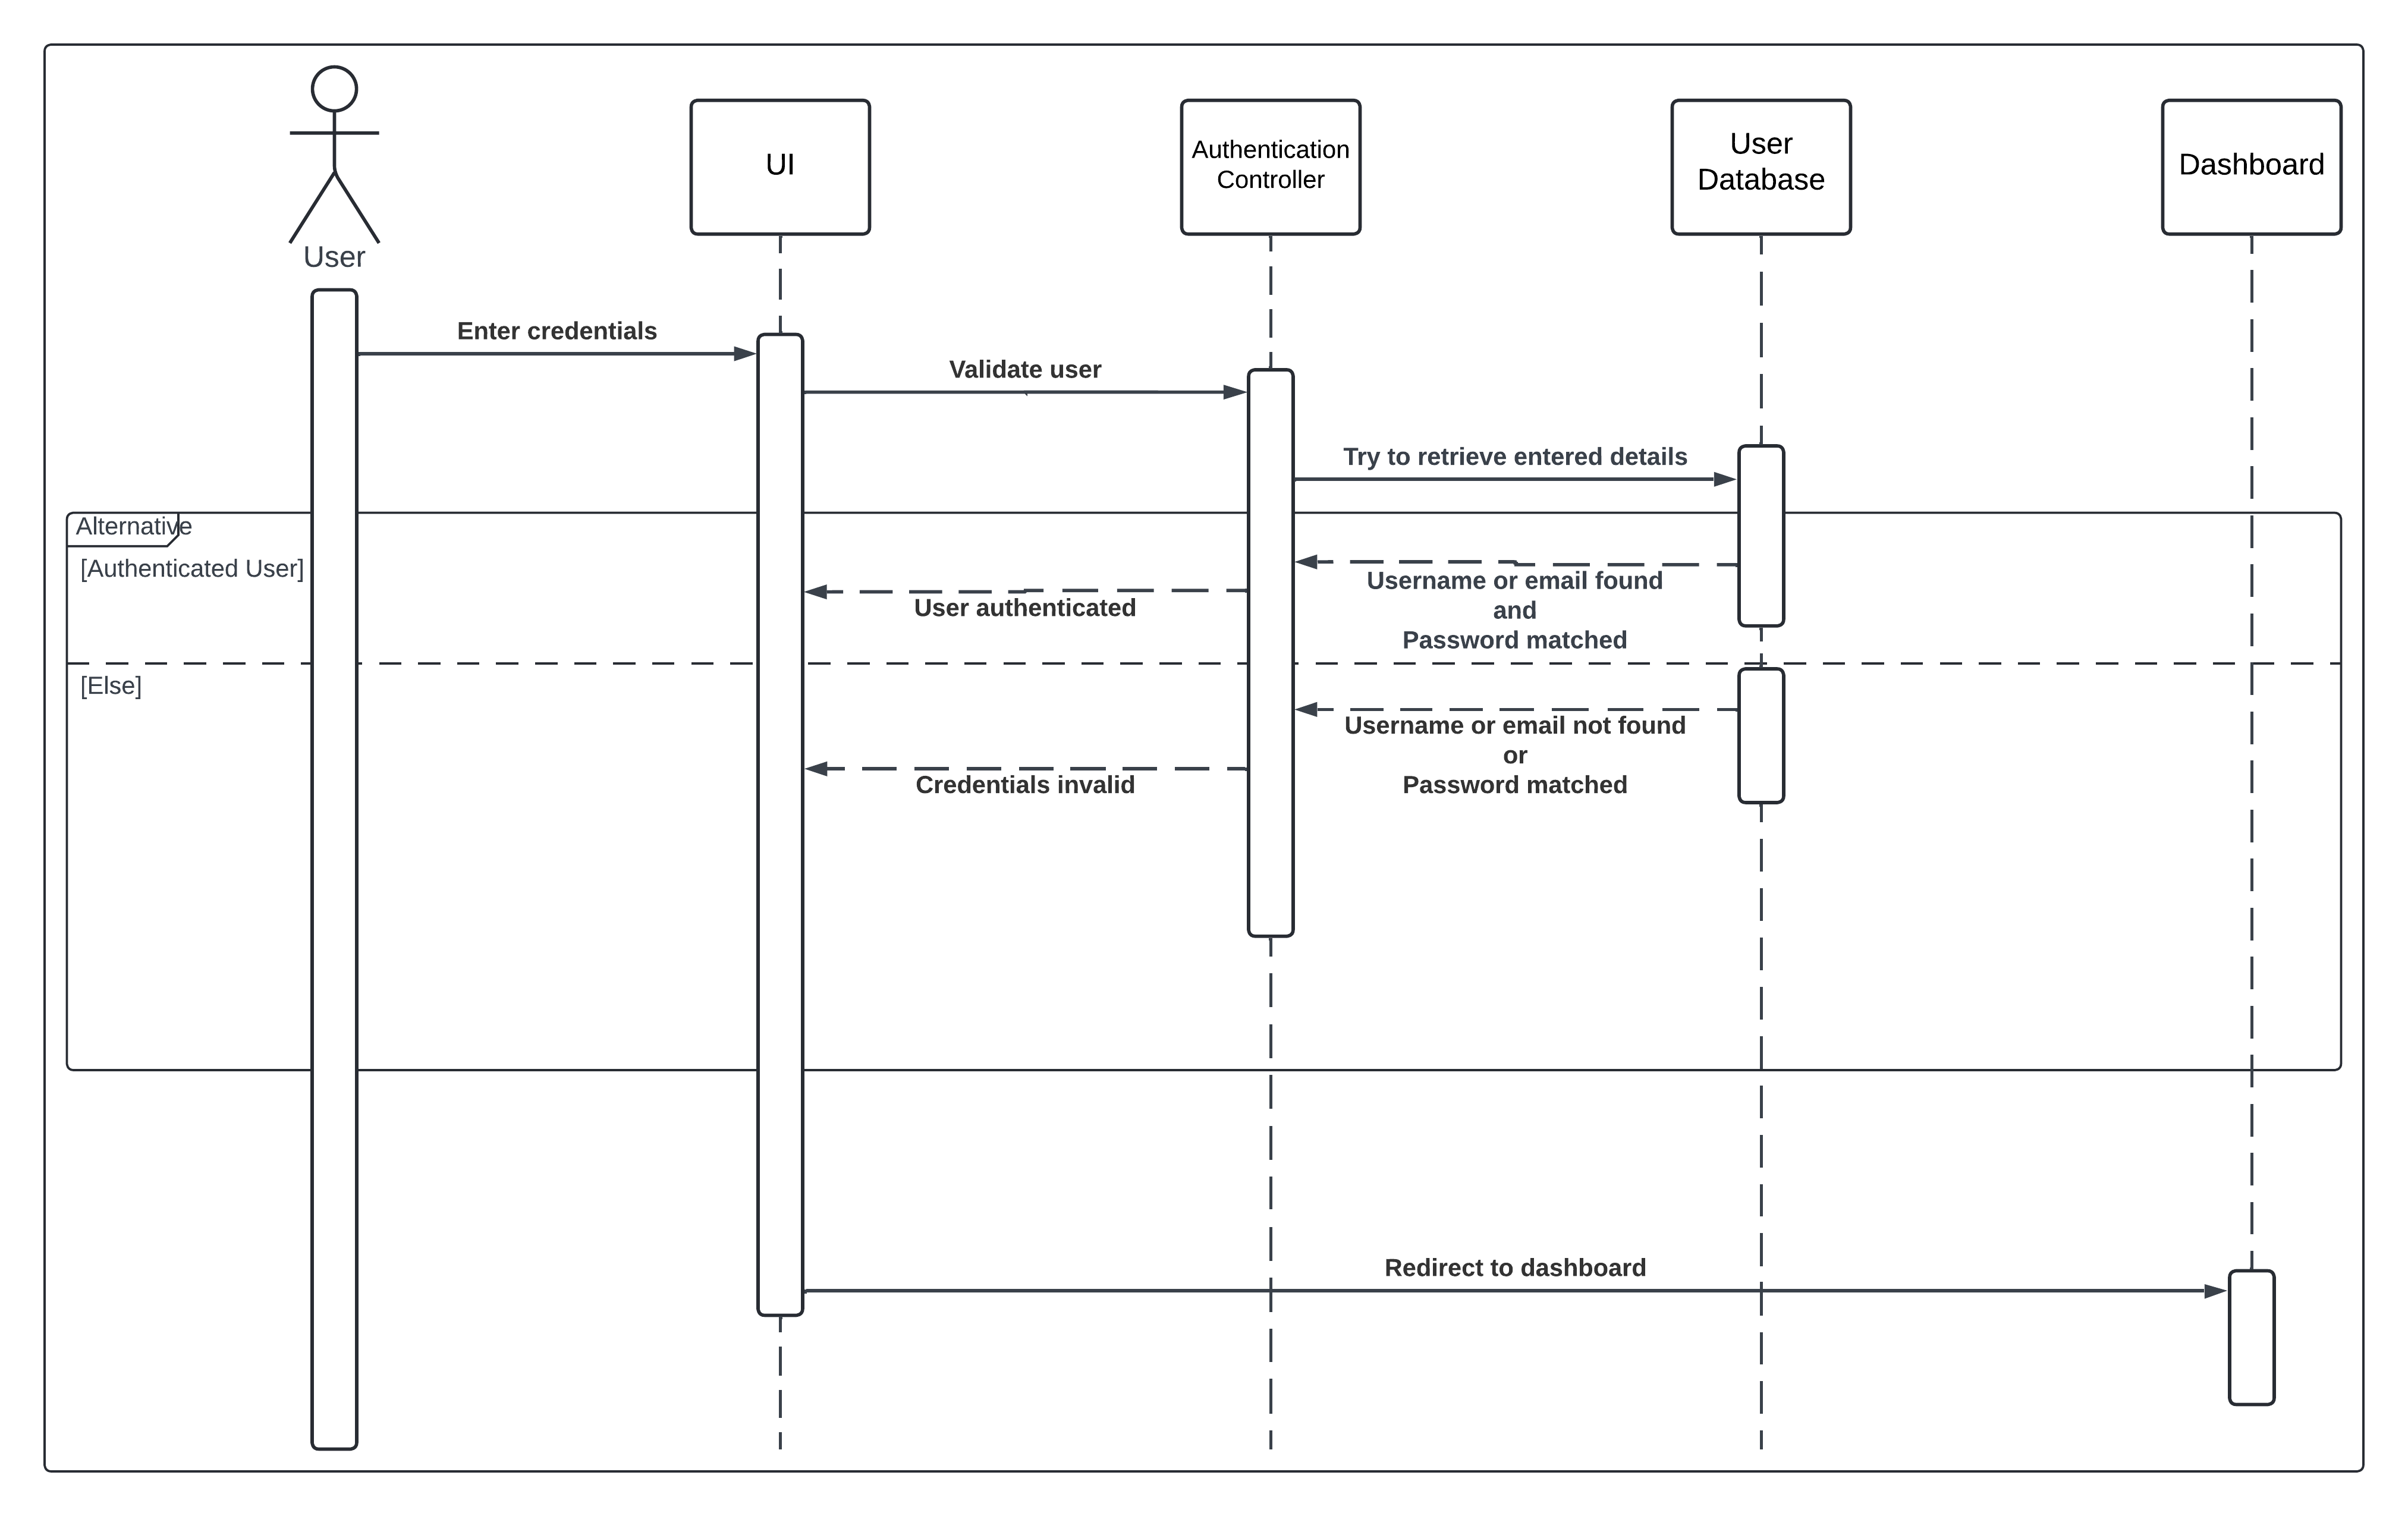
\includegraphics[width=16cm]{Images/login-sequence.png}
    \caption{Login Sequence Diagram}
    \label{fig:login-sequence}
\end{figure}
\begin{figure}[H]
    \centering
    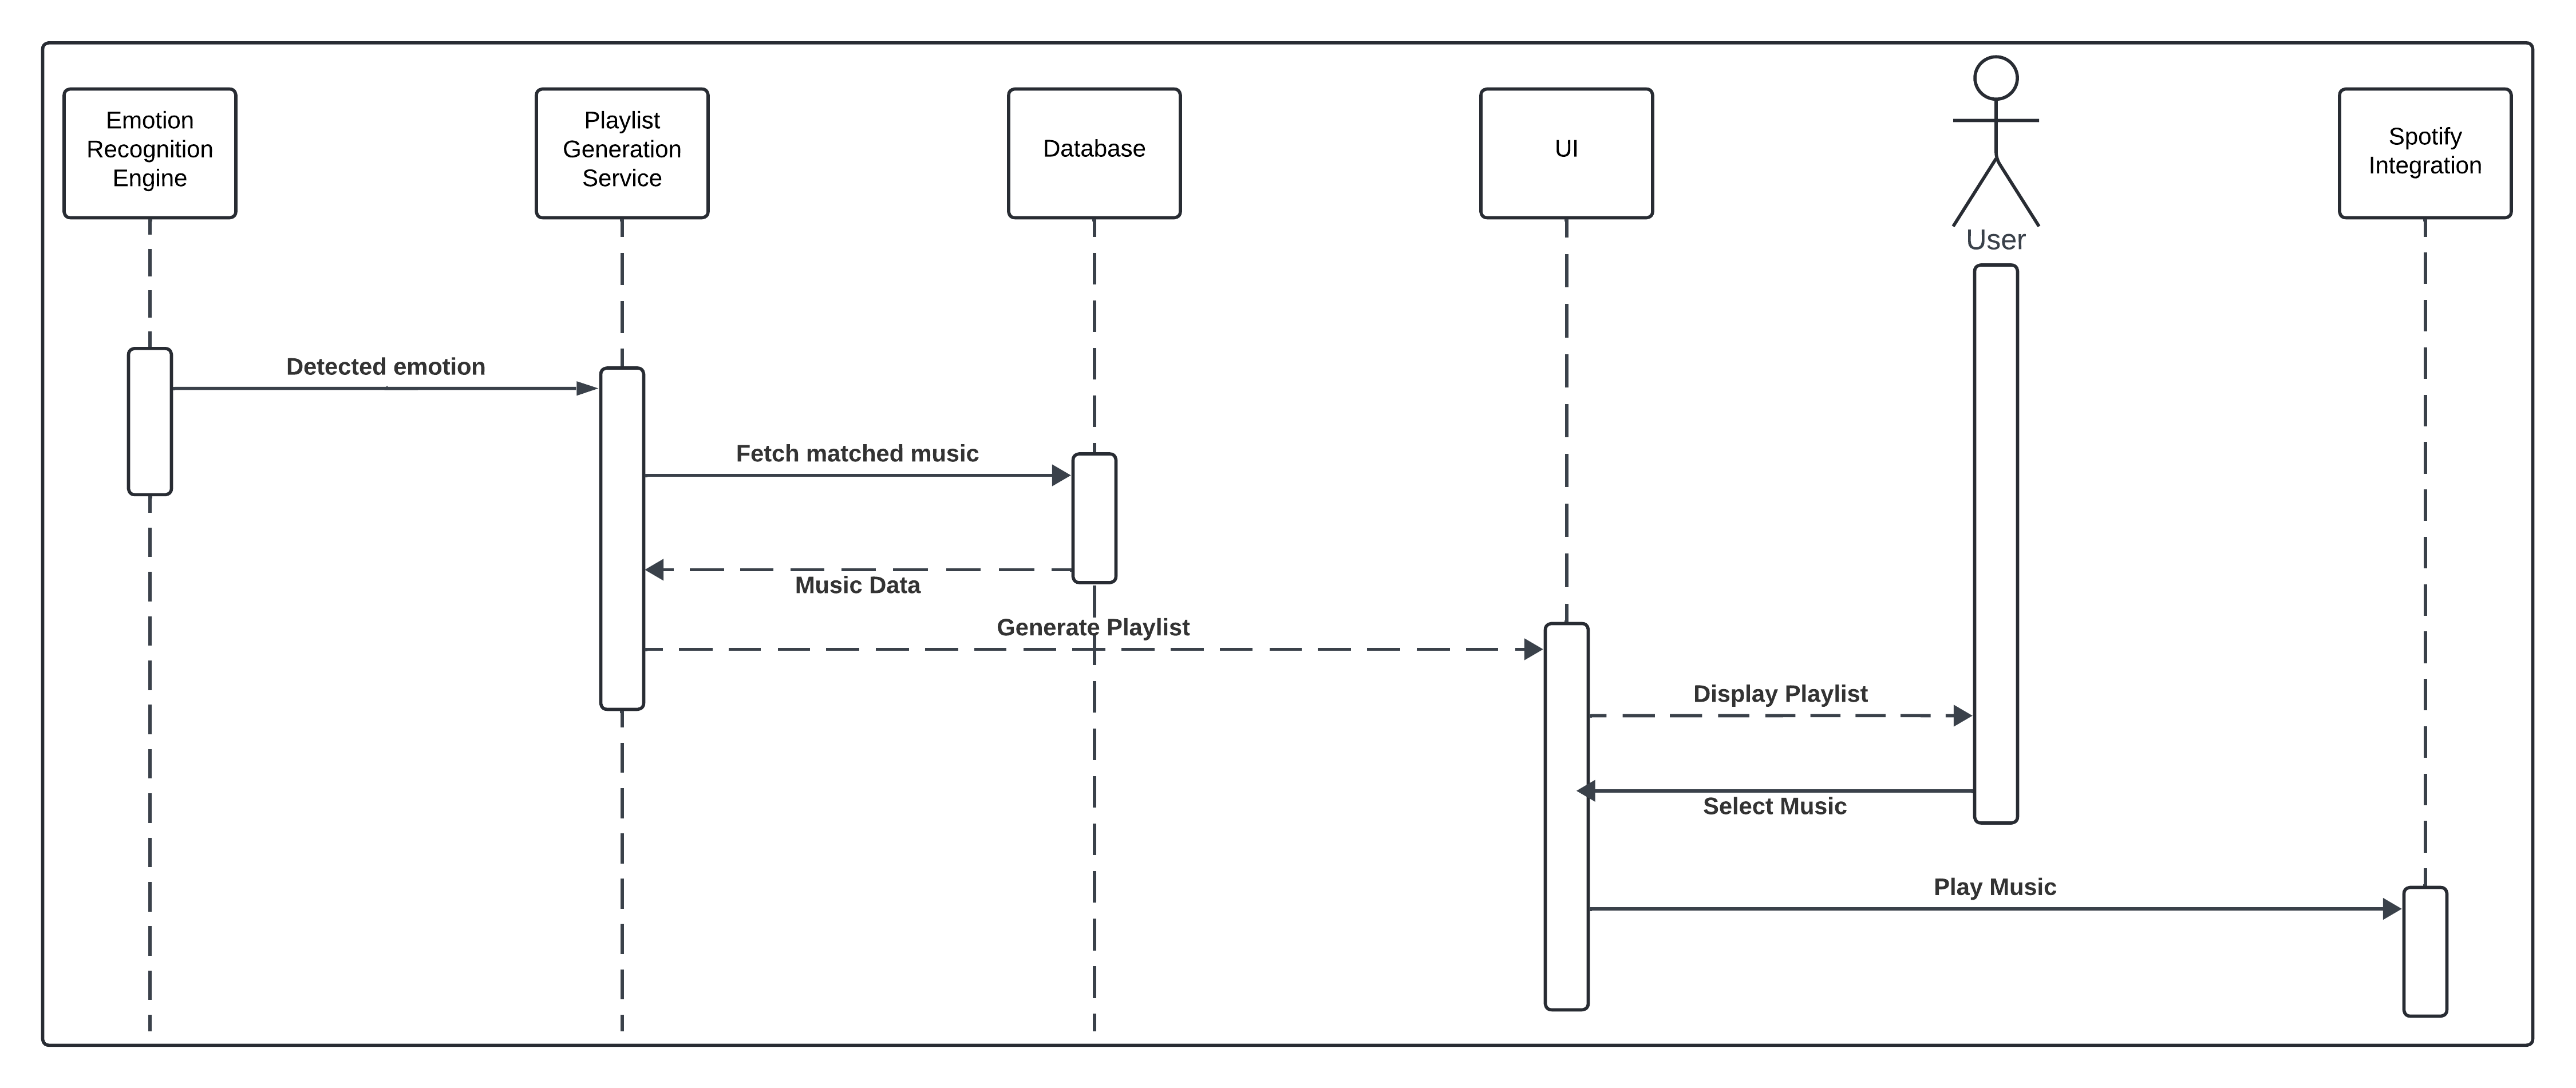
\includegraphics[width=16cm]{Images/playlist-sequence.png}
    \caption{Playlist Generation Sequence Diagram}
    \label{fig:playlist-sequence}
\end{figure}
\begin{figure}[H]
    \centering
    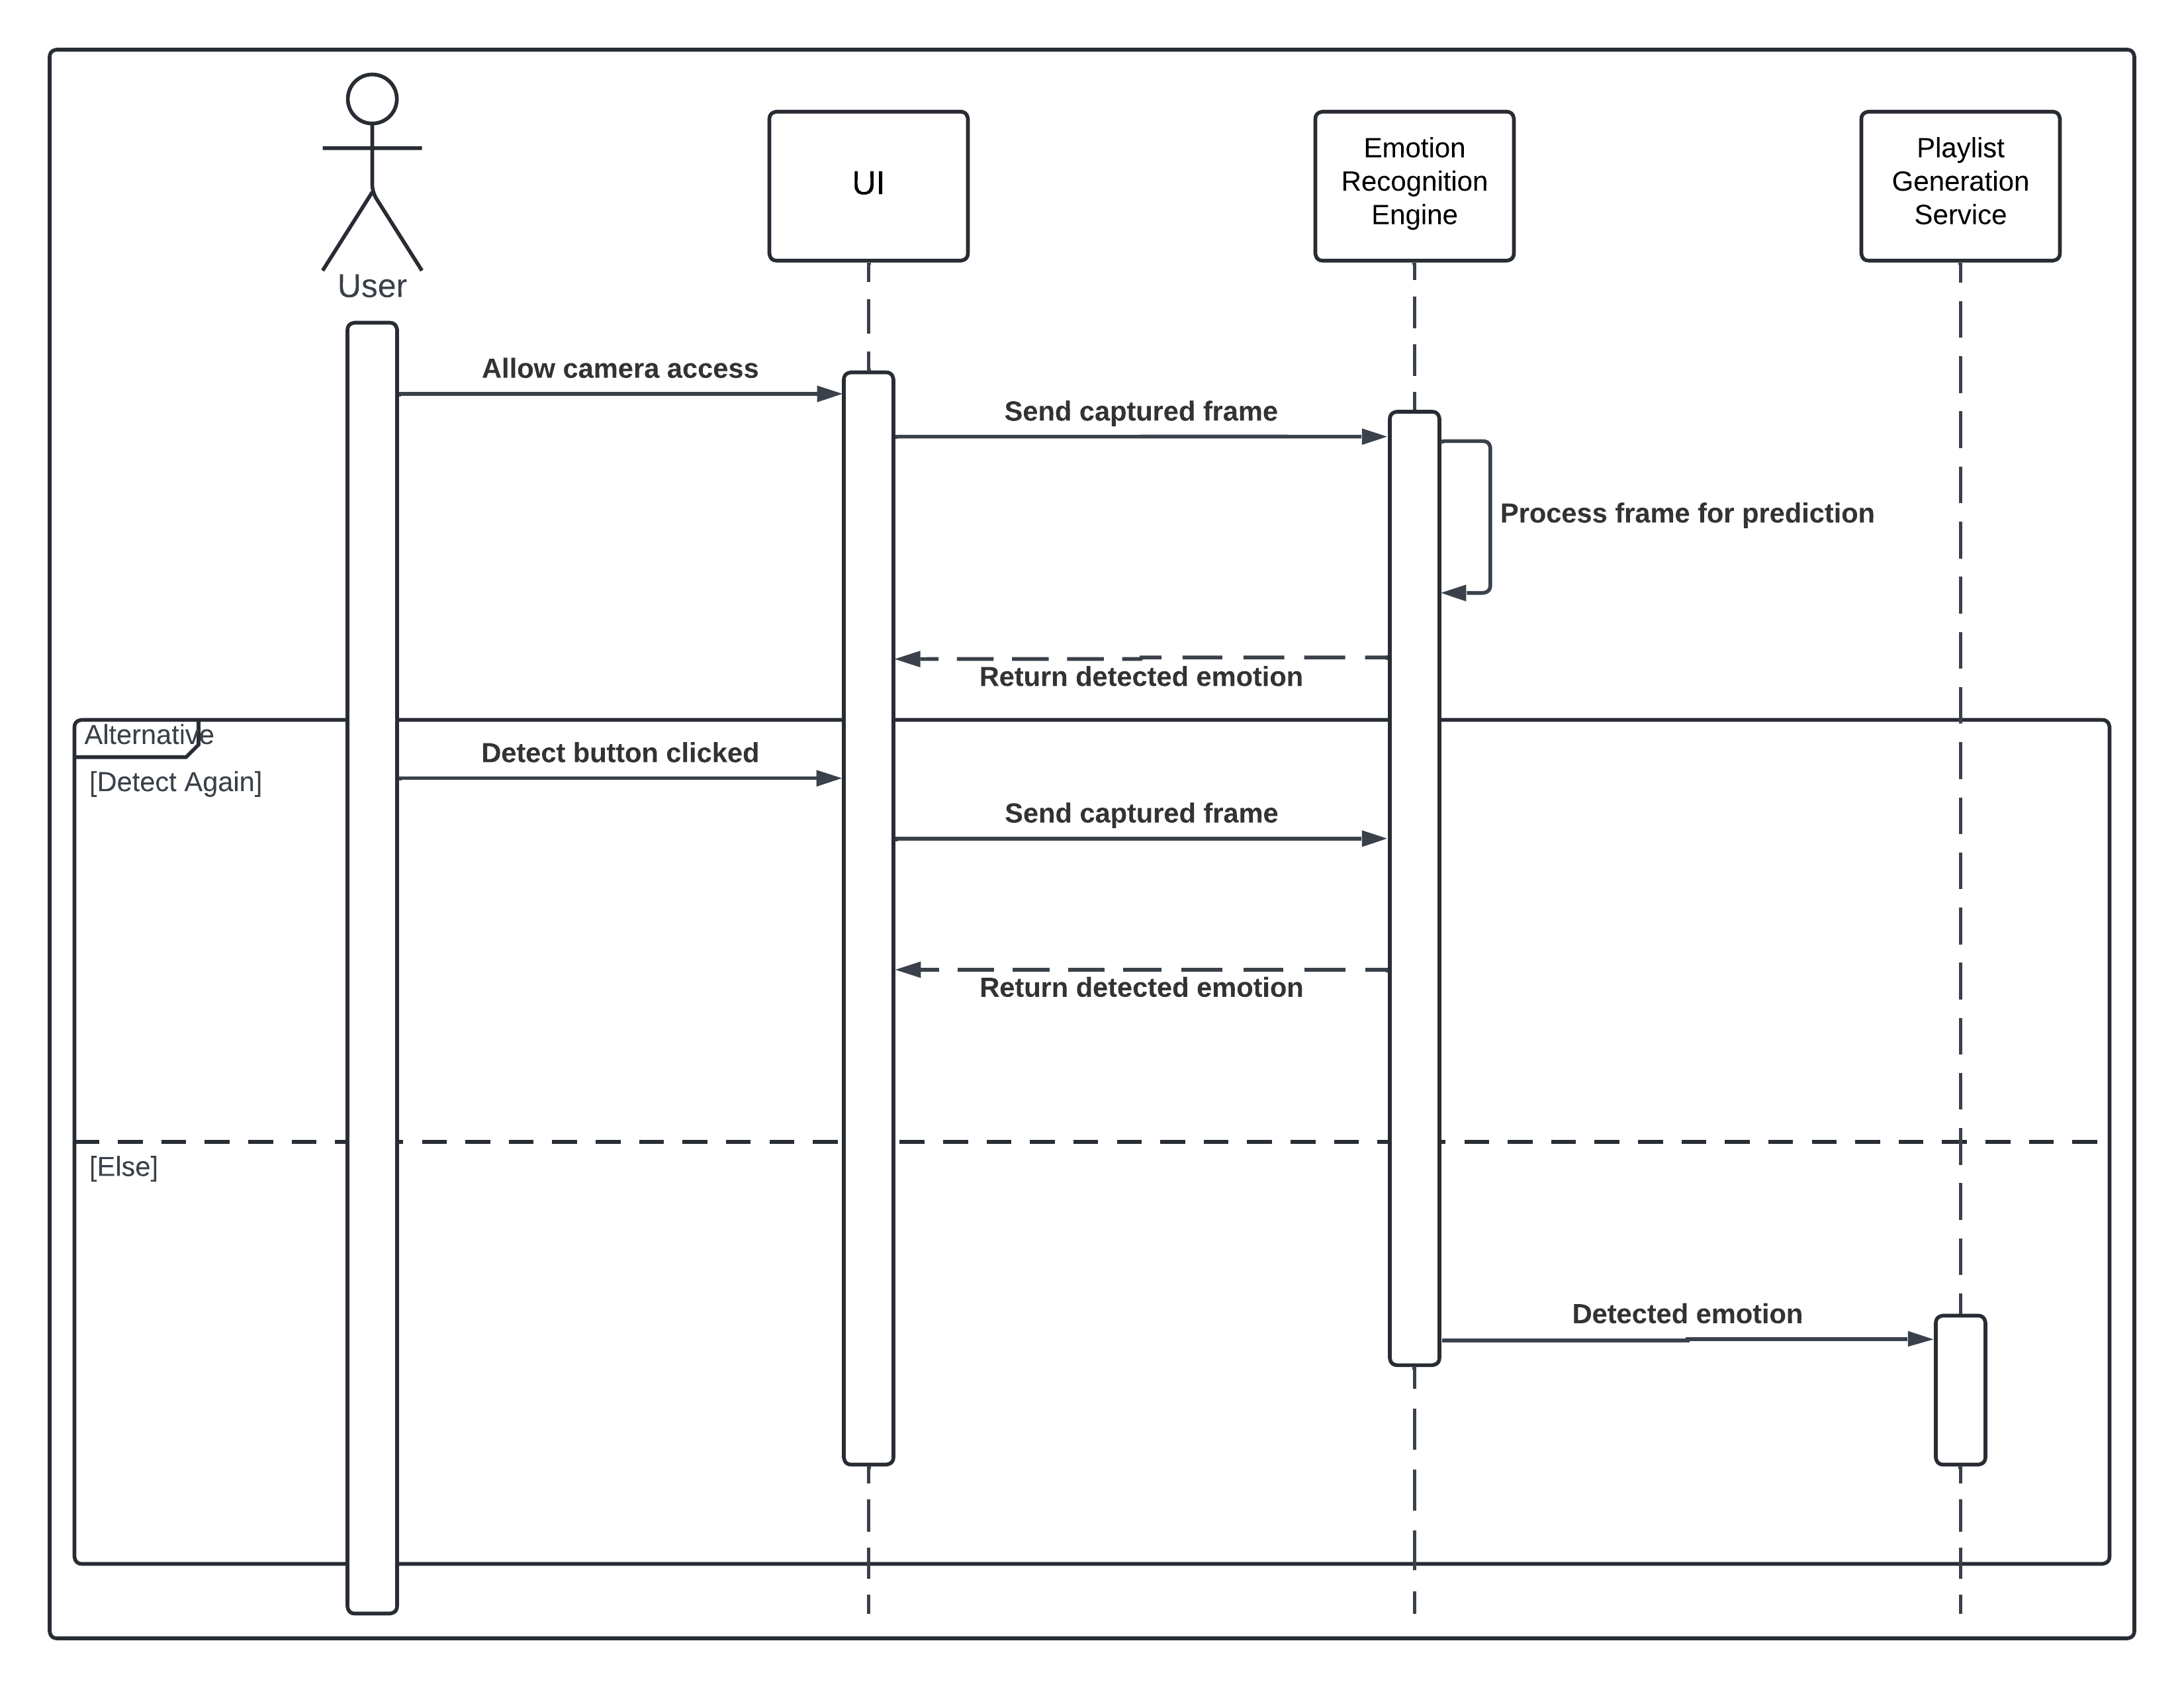
\includegraphics[width=16cm]{Images/fer-sequence.png}
    \caption{Emotion Recognition Sequence Diagram}
    \label{fig:fer-sequence}
\end{figure}
\indent Figure \ref{fig:fer-sequence} presents the series of interactions that commence with capturing a user's facial expression and terminates when the system identifies the user's emotional state.
The sequence is outlined from the user interface to the backend services, where the input is processed by the `Emotion Recognition Engine' to identify emotion. 
The detected emotion will then influence the music playlist generation. 
\\
\indent Figure \ref{fig:playlist-sequence} shows how the service uses the detected emotion from Figure \ref{fig:fer-sequence} to choose and assemble a series of songs into a coherent playlist.
From retrieving suitable songs based on the emotional analysis to returning the playlist to the user for playback through Spotify Web Playback service, it demonstrates the cooperation between the system's components.
\\
\subsubsection{Flowchart}
Flowchart represent the process of a system, the decisions that need to be made, and the flow of control from one step to the next.
Troubleshooting and system design are made considerably easier with the aid of flowchart as they make the sequential phase and logic paths in complicated processes visible \citep{lucidchart_2019_what}.
\begin{figure}[H]
    \centering
    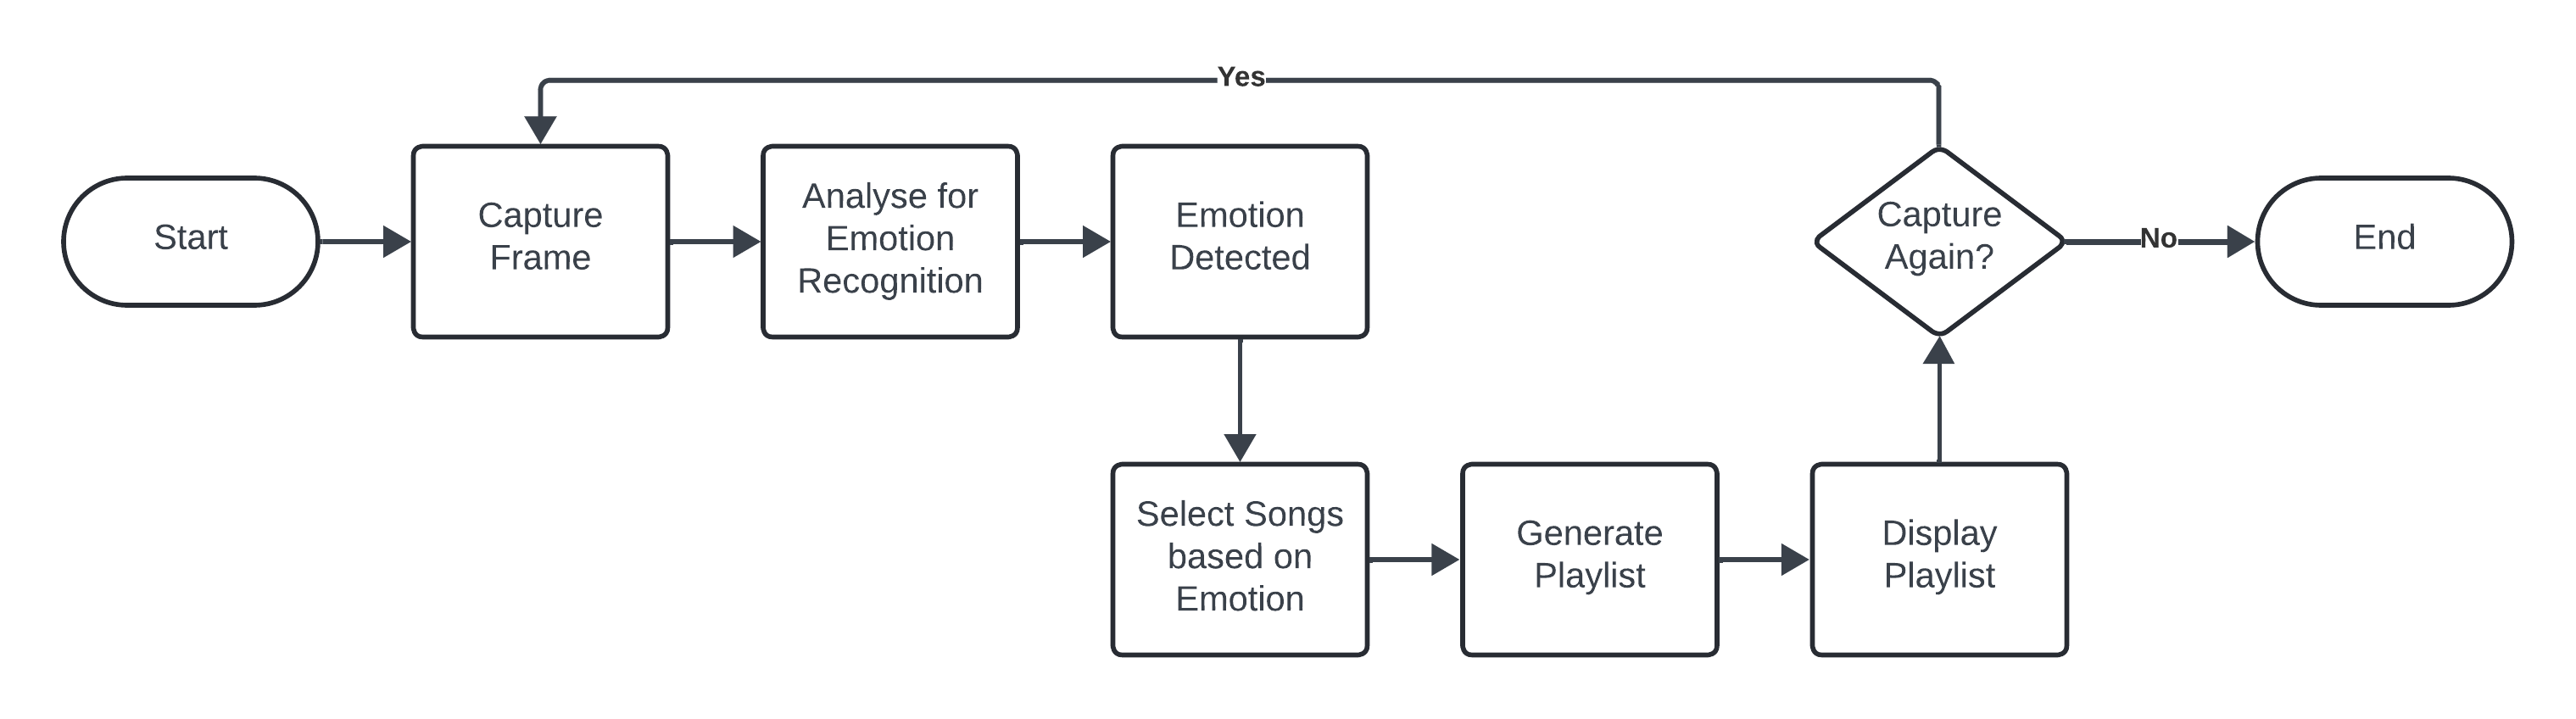
\includegraphics[width=16cm]{Images/flowchart.png}
    \caption{Flowchart For Emotion Recognition and Playlist Generation}
    \label{fig:flowchart-fer-pg}
\end{figure}
\indent Figure \ref{fig:flowchart-fer-pg} shows the steps taken from the moment a user engages with the feature to capture their emotional state to the point where the system recognizes and outputs the detected emotion.
Following the \gls{fer} phase, the identified emotion is then used to select suitable music, creating playlist and presenting it to the user. 
\\
\subsubsection{Entity-relationship Diagram}
\gls{erd} is a structured representation of the data entities within the web application and the interconnections between them. 
This illustration outlines the database schema, which is foundational for storing, retrieving, and managing data that the application operates upon.
\\
\indent Figure \ref{fig:erd} presents the \gls{erd} for the application.
`User' representing the application's users, containing `UserID', `Username' and other personal details which could be modified in `User Settings Page' (See Figure \ref{fig:usr-settings}).
`Albums', `Tracks', `Audio Features', `Track Popularity', and `Artists' are entities that stored music data from song title to information such as its tempo, its loudness and other audio features.
\begin{figure}[H]
    \centering
    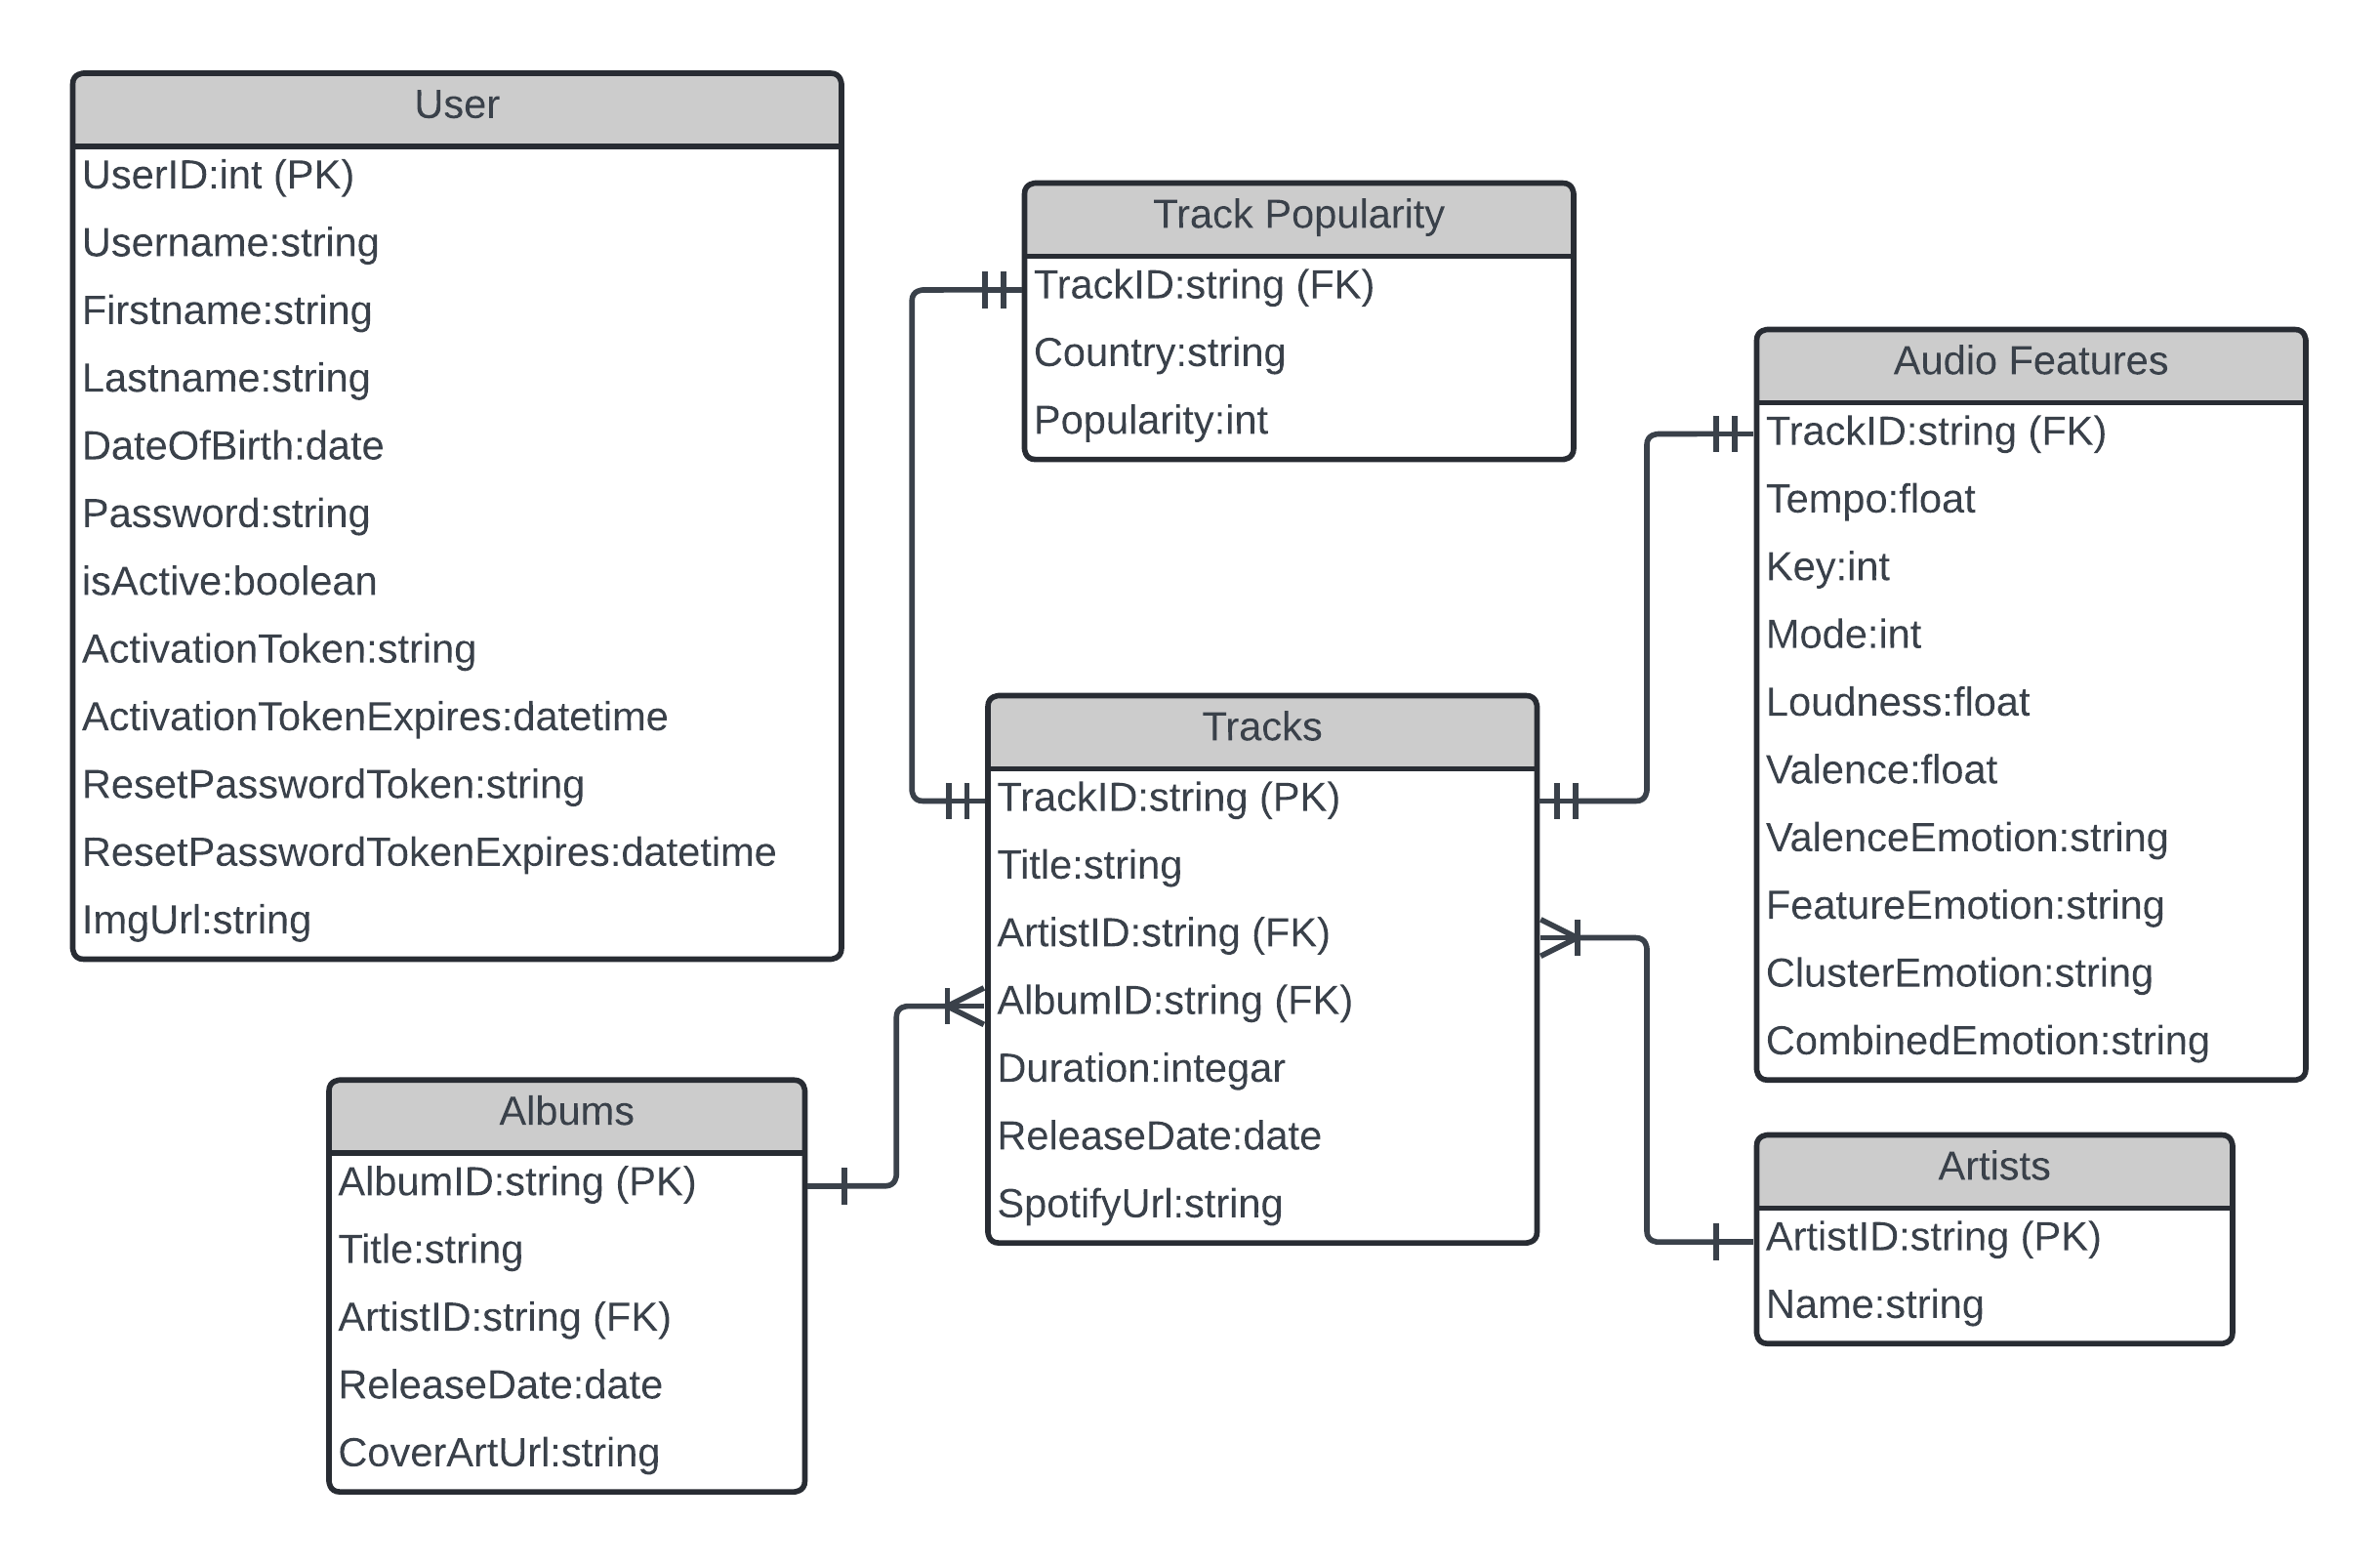
\includegraphics[width=16cm]{Images/erd.png}
    \caption{Entity-relationship Diagram}
    \label{fig:erd}
\end{figure}
\indent The relationship between entities are defined by \gls{pk} and \gls{fk}, enforcing referential integrity within the database.
For example, a one-to-many relationship from `Artists' to `Tracks' indicates that one artist can have multiple tracks, whereas a one-to-one relationship between `Tracks' and `Audio Features' indicates that each track has its own unique features.
\subsection{Logo Design}
Figure \ref{subfig:light-logo} and Figure \ref{subfig:dark-logo} is made up of stylized waves that reference the soothing rhythms of ocean waves while also visualizing the representation of an audio signal.
This duality shows the fundamental purpose of the application, using the ability of music to evoke and influence emotions, providing a calming and therapeutic user experience.
\indent Accompanying the logo, Figure \ref{subfig:light-banner} and Figure \ref{subfig:dark-banner} incorporates the application's name, `Sentirhy', which itself is a portmanteau derived from `Sentiment' and `Rhythm'.
This naming convention shows the application's focus on sentiment analysis and rhythm.
\begin{figure}[H]
    \centering
    \subfloat[\centering Logo \label{subfig:light-logo}]{{
\includegraphics[width=3cm]{Images/dark.png}}}%
    \qquad
    \subfloat[\centering Banner\label{subfig:light-banner}]{{
\includegraphics[width=7cm]{Images/dark-banner.png}}}%
    \vspace{0.5cm}
    \\
    \caption{Light Theme Logo}
\end{figure}
\begin{figure}[H]
    \centering
    \makebox[\textwidth]{
        \begin{minipage}{14cm} 
            \begin{mdframed}[backgroundcolor=gray!70]
                \centering
                \subfloat[\centering Logo \label{subfig:dark-logo}]{{
\includegraphics[width=3cm]{Images/light.png}}}%
                \qquad
                \subfloat[\centering Banner\label{subfig:dark-banner}]{{
\includegraphics[width=7cm]{Images/light-banner.png}}}%
            \end{mdframed}
        \end{minipage}
    }
    \caption{Dark Theme Logo}
\end{figure}
\subsection{Interface Design}
\gls{ui}s are created through the process of interface design.
The arrangement of panels, as well as the style of components the user will interact with such as buttons, text fields and others are all included (See Appendix D).
\begin{figure}[H]
    \centering
    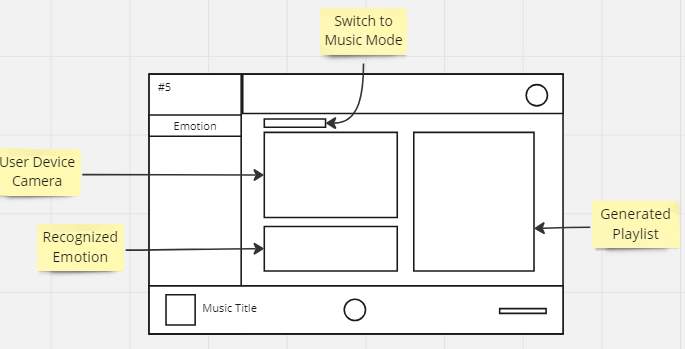
\includegraphics[width=12cm]{Images/detection.png}
    \caption{Emotion Recognition Page}
    \label{fig:emotion-recog}
\end{figure}

\section{Artificial Intelligence and Machine Learning}
\subsection{Models Architecture}
In computer vision, a model's architecture is the basis that backs up its capacity for learning and generalization.
The design decisions made when structuring a model determine not only its performance, but also its efficiency in extracting and understanding the complex patterns found in the data. 
A \gls{fer} model must be able to manage the complexity of human facial emotions with ease. 
Therefore, the architectures explored and selected are designed with the goal of capturing a complex hierarchy of features.
\begin{table}[H]
    \centering
    \begin{tabular}{>{\ttfamily}l>{\ttfamily}l>{\ttfamily}r}
        \toprule 
        \textbf{Layer (Type)} & \textbf{Output Shape} & \textbf{Parameters} \\
        \midrule
        Input & (None, 48, 48, 1) & 0 \\ 
        Conv2D (3x3x32) & (None, 48, 48, 32) & 320 \\
        Conv2D (3x3x64) & (None, 48, 48, 64) &  18,496\\
        BatchNormalization & (None, 48, 48, 64) & 256 \\
        MaxPooling2D (2x2) & (None, 24, 24, 64) & 0 \\
        Dropout & (None, 24, 24, 64) & 0 \\
        Conv2D (3x3x128) & (None, 24, 24, 128) & 73,856 \\
        Conv2D (3x3x256) & (None, 22, 22, 256) &  295,168\\
        BatchNormalization & (None, 22, 22, 256) & 1,024 \\
        MaxPooling2D (2x2) & (None, 11, 11, 256) & 0 \\
        Dropout & (None, 11, 11, 256) & 0 \\
        Flatten & (None, 30976) & 0 \\
        Dense & (None, 1024) & 31,720,448 \\
        Dropout & (None, 1024) & 0 \\
        Dense (Softmax) & (None, 4) & 4,100 \\
        \bottomrule 
    \end{tabular}
    \caption{Detailed Architecture of the CNNs Model 1}
    \label{tab:cnn-model-1}
\end{table}
\newpage
\indent Model 1 (See Table \ref{tab:cnn-model-1}) is the first attempt at tackling the challenging issue of \gls{fer}, based on the well-proven architectures similar to VGG-16 \citep{simonyan2015deep}, which are intended to identify nad leverage the strengths of facial feature differentiation.
The model started with a conservative number of filters in the \gls{conv2d}, from 32 and incrementally increasing to 64, 128, and 256, to ensure the model is able to capture a spectrum of features from basic to complex. 
Those interspersed `Dropout' layers are used to prevent over-fitting, which then giving the model greater generalization capabilities.
\\
\indent In order to reduce dimensionality, pooling layers are implemented throughout the architecture.
This will compress the spatial volume of features before they are flattened into a format suitable for dense network processing.
The learning process ends in the `Dense' layers that, through a `Softmax' activation, control the emotional categorization, converting the complex network of extracted features into perceptible emotional states.
\\
\indent Model 2 (See Table \ref{tab:cnn-model-2}) is a refined version of the \gls{fer} model.
With the addition of L2 regularization and a varied number of filter sizes, this model differs from the first model.
This version provides theoretical performance improvements, such as higher generalization in unseen data.
Additionally, this model version is more similar to the VGG-16 model; but, because of resource constraints, the original VGG-16 model, which in theory should yield better results, is not implemented in order to use fewer computer resources.
\begin{table}[H]
    \centering
    \begin{tabular}{>{\ttfamily}l>{\ttfamily}l>{\ttfamily}r}
        \toprule 
        \textbf{Layer (Type)} & \textbf{Output Shape} & \textbf{Parameters} \\
        \midrule 
        Input & (None, 48, 48, 1) & 0 \\
        Conv2D (3x3x64) & (None, 48, 48, 64) & 640 \\
        BatchNormalization & (None, 48, 48, 64) & 256 \\
        ReLU Activation & (None, 48, 48, 64) & 0 \\
        Conv2D (3x3x64) & (None, 48, 48, 64) & 36,928 \\
        BatchNormalization & (None, 48, 48, 64) & 256 \\
        ReLU Activation & (None, 48, 48, 64) & 0 \\
        MaxPooling2D (2x2, stride 2) & (None, 24, 24, 64) & 0 \\
        Conv2D (3x3x128) & (None, 24, 24, 128) & 73,856 \\
        BatchNormalization & (None, 24, 24, 128) & 512 \\
        ReLU Activation & (None, 24, 24, 128) & 0 \\
        Conv2D (3x3x128) & (None, 24, 24, 128) & 147,584 \\
        BatchNormalization & (None, 24, 24, 128) & 512 \\
        ReLU Activation & (None, 24, 24, 128) & 0 \\
        MaxPooling2D (2x2, stride 2) & (None, 12, 12, 128) & 0 \\
        Conv2D (3x3x256) & (None, 12, 12, 256) & 295,168 \\
        BatchNormalization & (None, 12, 12, 256) & 1,024 \\
        ReLU Activation & (None, 12, 12, 256) & 0 \\
        Conv2D (3x3x256) & (None, 12, 12, 256) & 590,080 \\
        BatchNormalization & (None, 12, 12, 256) & 1,024 \\
        ReLU Activation & (None, 12, 12, 256) & 0 \\
        Conv2D (3x3x256) & (None, 12, 12, 256) & 590,080 \\
        BatchNormalization & (None, 12, 12, 256) & 1,024 \\
        ReLU Activation & (None, 12, 12, 256) & 0 \\
        MaxPooling2D (2x2, stride 2) & (None, 6, 6, 256) & 0 \\
        Flatten & (None, 9216) & 0 \\
        Dense & (None, 4096) & 37,752,832 \\
        BatchNormalization & (None, 4096) & 16,384 \\
        ReLU Activation & (None, 4096) & 0 \\
        Dense & (None, 4096) & 16,781,312 \\
        BatchNormalization & (None, 4096) & 16,384 \\
        ReLU Activation & (None, 4096) & 0 \\
        Dense (Softmax) & (None, 4) & 16,388 \\ 
        \bottomrule 
    \end{tabular}
    \caption{Detailed Architecture of the CNNs Model 2}
    \label{tab:cnn-model-2}
\end{table}
   
    
     % Section/Chapter entries can be done in the Main.tex file or in a  
                       % separate tex file for longer and more complex documents

% -------------------  IMPLEMENTATION  ---------------------
\chapter{Implementation}
\section{Introduction}
This section covers how the research was put into practice, with a particular emphasis on how machine learning models were put into practice and how they were integrated into a working web application for \gls{fer}.
\section{Artificial Intelligence and Machine Learning}
The preparation of datasets, the training environment, and the computational resources employed will be discussed in the following section.
Providing specific details about the measures taken to guarantee that the data was suitable for learning, the augmentation methods used to improve model performance, and the training approaches used to maximize model performance.
The evaluation metrics and the outcome of testing the models on hypothetical data are also included in this \gls{ml} section.
\subsection{Setup and Preparation}
\subsubsection{Environment Setup}
The models are developed with a robust software environment designed for advanced \gls{ml} tasks.
The preferred programming language was Python \citep{python_2019_python}, which is well-known for its adaptability and power in data manipulation and machine learning.
Then, the research and model training were carried out with Jupyter Notebook \citep{jupyter_2019_project}, which is an interactive computing environment that enables real-time code execution, analysis and visualization.
The libraries used for model training are listed below.
\begin{itemize}
    \item \textbf{Keras}: Chosen for its user-friendly API which operates on top of TensorFlow, it enabled to build and train neural network models with relative ease. \citep{team_keras}
    \item \textbf{NumPy}: It is used for handling of numerical operations on array, forming the foundation of data structures in \gls{ml} tasks. \citep{numpy_2009_numpy}
    \item \textbf{Pandas}: This library provided robust data manipulation and cleaning capabilities which makes organizing tabular data and dataset transformation more easier. \citep{pandas_2018_python}
    \item \textbf{Scikit-learn (sklearn)}: A broad range of machine learning tools, including cross-validation methods, model assessment, and preprocessing, are available in this library and aid in the improvement of learned models. \citep{scikitlearn_2019_scikitlearn}
    \item \textbf{OpenCV (cv2)}: This library provided extensive image processing capabilities, which were crucial in manipulating and preparing facial images for training. \citep{opencv_2019_opencv}
    \item \textbf{Matplotlib and Seaborn}: These libraries were used for data visualization. They allow findings to be converted into charts, which provide further insight into the functioning of the models. \citep{matplotlib_2012_matplotlib} \citep{seaborn_2012_seaborn}
\end{itemize}
\subsubsection{Data Preparation}
\paragraph{Data Collection}
\begin{figure}[h!]
    \centering
    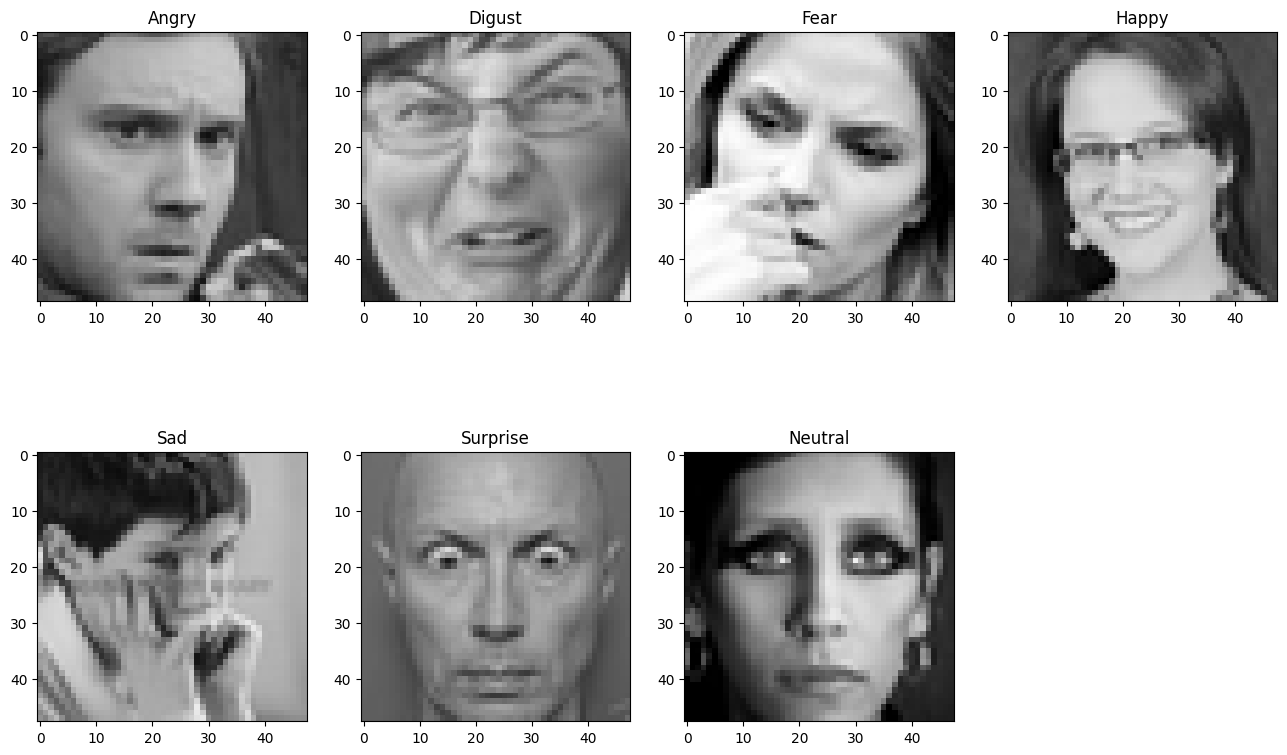
\includegraphics[width=10cm]{Images/fer2013.png}
    \caption{FER-2013 Dataset}
    \label{fig:fer2013}
\end{figure}
A dataset capable of precisely capturing a wide range of human emotions through facial expression was needed for training the model. 
Therefore, the FER-2013 \citep{challenges_in_representation_learning_facial_expression_recognition_challenge} dataset which is a well-known benchmark in the field of  \gls{fer} from the Kaggle competition platform was chosen.
A wide range of facial expressions are included in this dataset, and each of these grayscale images of faces are labelled with one of seven emotions.
This makes it suited for training \gls{fer} models.
\begin{figure}[h!]
    \centering
    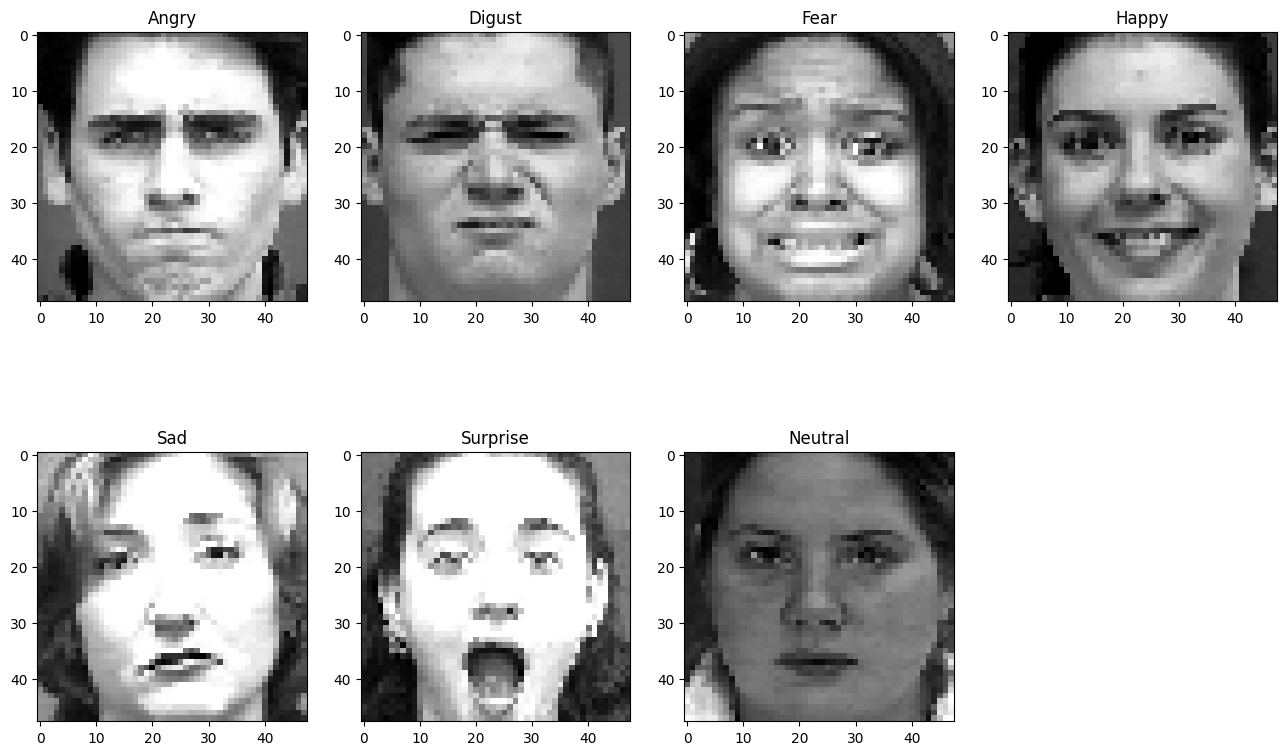
\includegraphics[width=10cm]{Images/ckextended.png}
    \caption{CK+ Dataset}
    \label{fig:ckextended}
\end{figure}
\\
\indent To increase the diversity of the data, CK+ \citep{5543262} dataset is included to the FER-2013. 
This dataset contains labelled facial expressions from varied populations and light scenarios.
This addition was to provide the models a more comprehensive learning environment by exposing them to a greater variety of face emotions and characteristics.
\begin{figure}[h!]
    \centering
    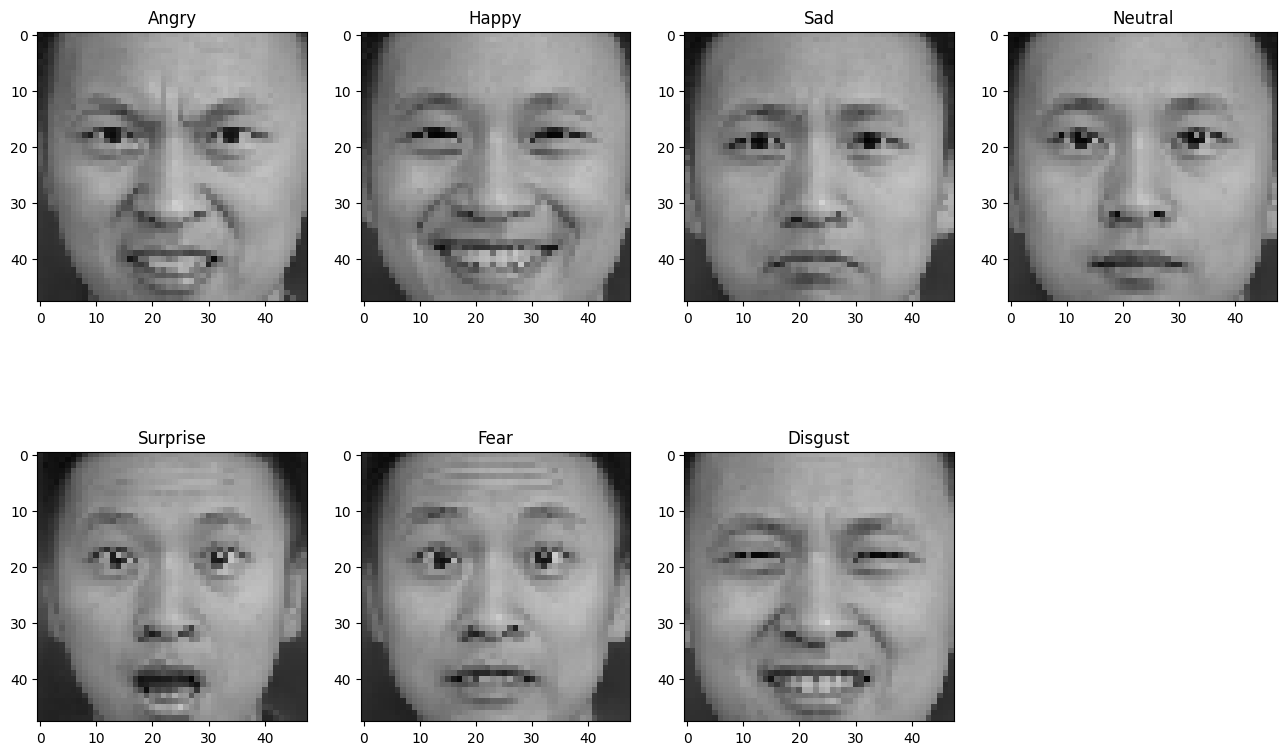
\includegraphics[width=10cm]{Images/szuemodage.png}
    \caption{SZU-EmoDage Dataset}
    \label{fig:szu-emodage}
\end{figure}
\\
\indent Moreover, SZU-EmoDage \citep{who_2022_a} dataset was also included to the collection to ensure the models are capable of identifying facial expressions on Asian faces.
With these additions, each dataset was integrated with a different set of challenges and viewpoints, which then improve the model's accuracy and practicality in real-world situation.
\paragraph{Preprocessing Steps}
Those collected data went through a series of preprocessing stages to standardize input features and optimize them for efficient \gls{ml} before training.
Even though the data were already in grayscale, all images were first converted to grayscale using the \texttt{cv2.cvtColor(image, cv2.COLOR\_BGR2GRAY)} function to ensure that all data were in grayscale in order to simplify the input data and reduce computational cost.
After conversion, all images were shrunk to 48x48 pixels.
It is because neural networks require consistent picture sizes in order to handle batch data efficiently and handle all inputs equally during the learning process.
\\
\indent Following resizing, images were flattened from a format of 2D arrays to a 1D array with 2304 elements (48x48). 
This transformation is necessary because machine learning algorithms generally require a flat array of features for each sample to be handle and analyse.
The flattened image data was then compiled into a pandas DataFrame, which made data handling and analysis in Python simpler.
Before training models, pixel values from each image were standardized to lie within the range of [0,1]. 
This normalization make sure that all input characteristics contribute equally to the model's learning because having different scale will influence the results.
\\
\indent In order to simplify the model and better match the project with its use in music recommendation, the number of emotion categories was cut down from seven to four.
The four categories were kept were `Neutral', `Happy', `Sad' and `Angry'.
These emotions are more easily applied and useful for determining musical mood.
\paragraph{Augmentation}
Keras' function `\texttt{ImageDataGenerator()}' is used to construct a strategic data augmentation process that improved the model's robustness and allowed it to generalize across a variety of face emotions and situations.
The augmentation techniques that were used included random rotation of images up to \(10^\circ\).
This mimics the natural tilts that occur in expressive moments.
Additionally, width and height shifts, which translate images by up to 10\% of their size in both directions.
This helps with situations when faces are not in the center of the frame.
\\
\indent To help the model learn to identify emotions from faces at different camera distances, random zooming was also applied to some of the images.
Moreover, the images were arbitrarily rotated horizontally so that the model could be trained on mirror copies of faces, therefore double the range of face orientations the model saw in the training.
\paragraph{Dataset Splitting}
A key phase in preparing for training and evaluation of \gls{ml} models is splitting the dataset into training, validation, and testing sets. 
The training set was composed from the `Training' data from FER-2013 and the complete CK+ dataset.
This is to increase the model's capacity to generalize across various demographic groups and emotional states by exposing it too a greater variety of facial expressions and environmental factors.
\\
\indent For validation, the `PublicTest' subset of the FER-2013 was used.
This collection is essential for adjusting the hyper-parameters of the model and for providing an unbiased evaluation of the model's fit on the training dataset.
The `PrivateTest' subset of the FER-2013 was used to do the final evaluation of the model's performance.
In addition to the training, validation, and testing data, SZU-EmoDage dataset is used specifically for transfer learning purpose. 
\subsection{Training Process}
\begin{figure}[h!] 
    \centering
\begin{minted}[frame=lines, framesep=2mm, baselinestretch=1.2, fontsize=\footnotesize, linenos]{python}
    param_grid = {
        'conv_1_filters': [32, 64],
        'conv_2_filters': [64, 96, 128],
        'conv_3_filters': [128, 192, 224],
        'conv_4_filters': [128, 160, 224, 256],
        'conv_1_kernel': [3, 6, 8],
        'conv_2_kernel': [3, 5, 8],
        'conv_3_kernel': [3, 5, 8],
        'conv_4_kernel': [3, 5, 8],
        'dropout_1': [0.1, 0.2, 0.4],
        'dropout_2': [0.0, 0.2, 0.3],
        'dropout_3': [0.0, 0.2, 0.3, 0.4],
        'dense_units': [512, 768, 1024],
        'l1_reg': [0.01, 0.001, 0.0001],
        'optimizer': ['adam', 'sgd'],
        'learning_rate': [1e-2, 1e-3, 1e-4], 
        'epochs': [10, 50, 100]
    }
\end{minted}
    \caption{Parameter Grid}
    \label{fig:param_grid}
\end{figure}
In the training process, a common training framework was introduced for both models (Table \ref{tab:cnn-model-1} and Table \ref{tab:cnn-model-2}) to ensure consistency in the methodological approach.
But some specific adjustments to address the unique characteristics of each model is allowed.
The training process started with a thorough grid search to optimize hyper-parameters including dropout rates, kernel sizes, convolutional filter counts, and dense layer unit counts.
Both models shared the same parameter grid as Figure \ref{fig:param_grid}.
This approach made it easier to explore the configuration space in an organized way, ensuring that each model was tuned to perform optimally.
\\
\indent After searching through the parameter grid (\ref{app:appendix-a}), the process focuses on configuring each model's architecture to best capture the nuances of facial expression for \gls{fer}.
Model 1 (Table \ref{tab:cnn-model-1}) has a relatively simple architecture, which require careful tuning if dropout rates and filter sizes to balance feature learning against the risk of over-fitting.
Model 2 (Table \ref{tab:cnn-model-2}) has more additional layers to capture a richer set of features before the final classification layer . 
But this led to a more thorough analysis required for the network's depth in relation to its performance on the validation set, which assisted in identifying when to add dropout and how to adjust the pooling layers.  
\\
\begin{figure}[h!] 
    \centering
\begin{minted}[frame=lines, framesep=2mm, baselinestretch=1.2, fontsize=\footnotesize, linenos]{python}
    es = EarlyStopping(monitor='val_accuracy', patience=5, restore_best_weights=True)
\end{minted}
    \caption{Early Stopping}
    \label{fig:earlystopping}
\end{figure}
\\
\indent To prevent over-fitting, early stopping mechanism, which configured as `EarlyStopping' callback (Figure \ref{fig:earlystopping}), is integrated into the training to monitor validation accuracy and automatically halt training if no improvement was detected for five consecutive epochs.
Most important of all, the callback (Figure \ref{fig:earlystopping}) was set to restore the weights form the epoch with the best validation accuracy, ensuring that the model maintained any progress made prior to the plateau.
This approach allows to train the model as long as beneficial, in the meantime, avoiding over-fitting and maintaining the optimal state achieved during training.
\\
\begin{figure}[h!] 
    \centering
\begin{minted}[frame=lines, framesep=2mm, baselinestretch=1.2, fontsize=\footnotesize, linenos]{python}
    steps_per_epoch=len(train_X) / batch_size
\end{minted}
    \caption{Steps per epoch}
    \label{fig:steps_per_epoch}
\end{figure}
\\
\indent Furthermore, the `\texttt{steps\_per\_epoch}' (Figure \ref{fig:steps_per_epoch}) parameter was calculated to ensure that each epoch processed the entire dataset.
With these techniques, early stopping and calculated epoch steps, the models were able to achieve a balance between computational prudence and strong learning.
Consequently, the models were well-positioned for dependable performance in \gls{fer}, having learned from training data efficiently and been prevented from the risk of over-fitting. 
\subsection{Model Evaluation}

\subsection{Model Comparison and Selection}
\begin{table}[ht]
    \centering
    \renewcommand{\arraystretch}{1.5}
    \begin{tabular*}{\textwidth}{@{\extracolsep{\fill}}lcr}
    \toprule
    \textbf{Property} & \textbf{Model 1} & \textbf{Model 2} \\
    \midrule
    Input shape & 48 x 48 x 1 & 48 x 48 x 1 \\
    Weight layers & 6 & 10 \\
    Conv layers & 4 & 7 \\
    Kernel size & 3x3 & 3x3 \\
    Training params & 32,113,028 & 56,303,556 \\
    Model size & - & - \\
    Accuracy (\%) & 72.36 & - \\
    \bottomrule
    \end{tabular*}
    \caption{Comparison of Model 1 with Model 2}
    \label{tab:comparison-models}
\end{table}
\section{Web Application}
\begin{figure}[h!]
    \centering
    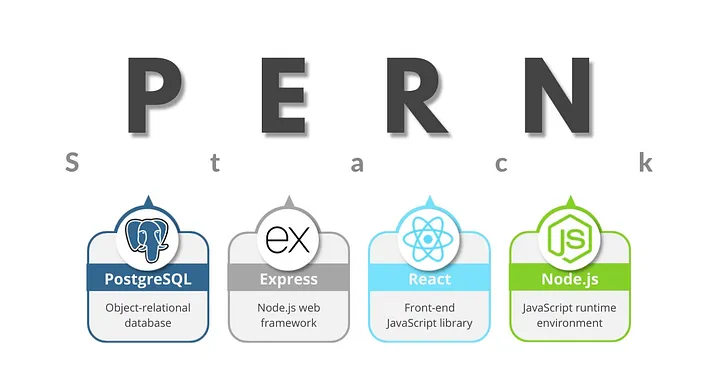
\includegraphics[width=10cm]{Images/pern.png}
    \caption{PERN Stack \citep{alves_2023_get}}
    \label{fig:pern}
\end{figure}
The web application uses the PERN stack (Figure \ref{fig:pern}), which is an acronym for PostgreSQL \citep{thepostgresqlglobaldevelopmentgroup_2019_postgresql}, Express \citep{openjsfoundation_2017_express}, React \citep{metaopensource_2024_react} and Node.js \citep{nodejs_2023_nodejs}.
This set of technologies provides a comprehensive end-to-end foundation for creating dynamic web application.
\\
\indent The frontend was built with React.js, a widely-used \gls{js} \gls{ui} framework, which was chosen for its declarative and effective method of creating \gls{ui}.
For the backend, Node.js was chosen for its non-blocking, event-driven architecture.
This architecture is well-suited for managing workloads that involve asynchronous operations, real-time applications and I/O-bound tasks.
The backend API is then constructed using Express.js, a simple and adaptable Node.js web application framework.
PostgreSQL is the chosen database system as it is well-known for its advanced features, data integrity and robustness.
\subsection{Login and Registration}
\begin{figure}[h!]
    \centering
    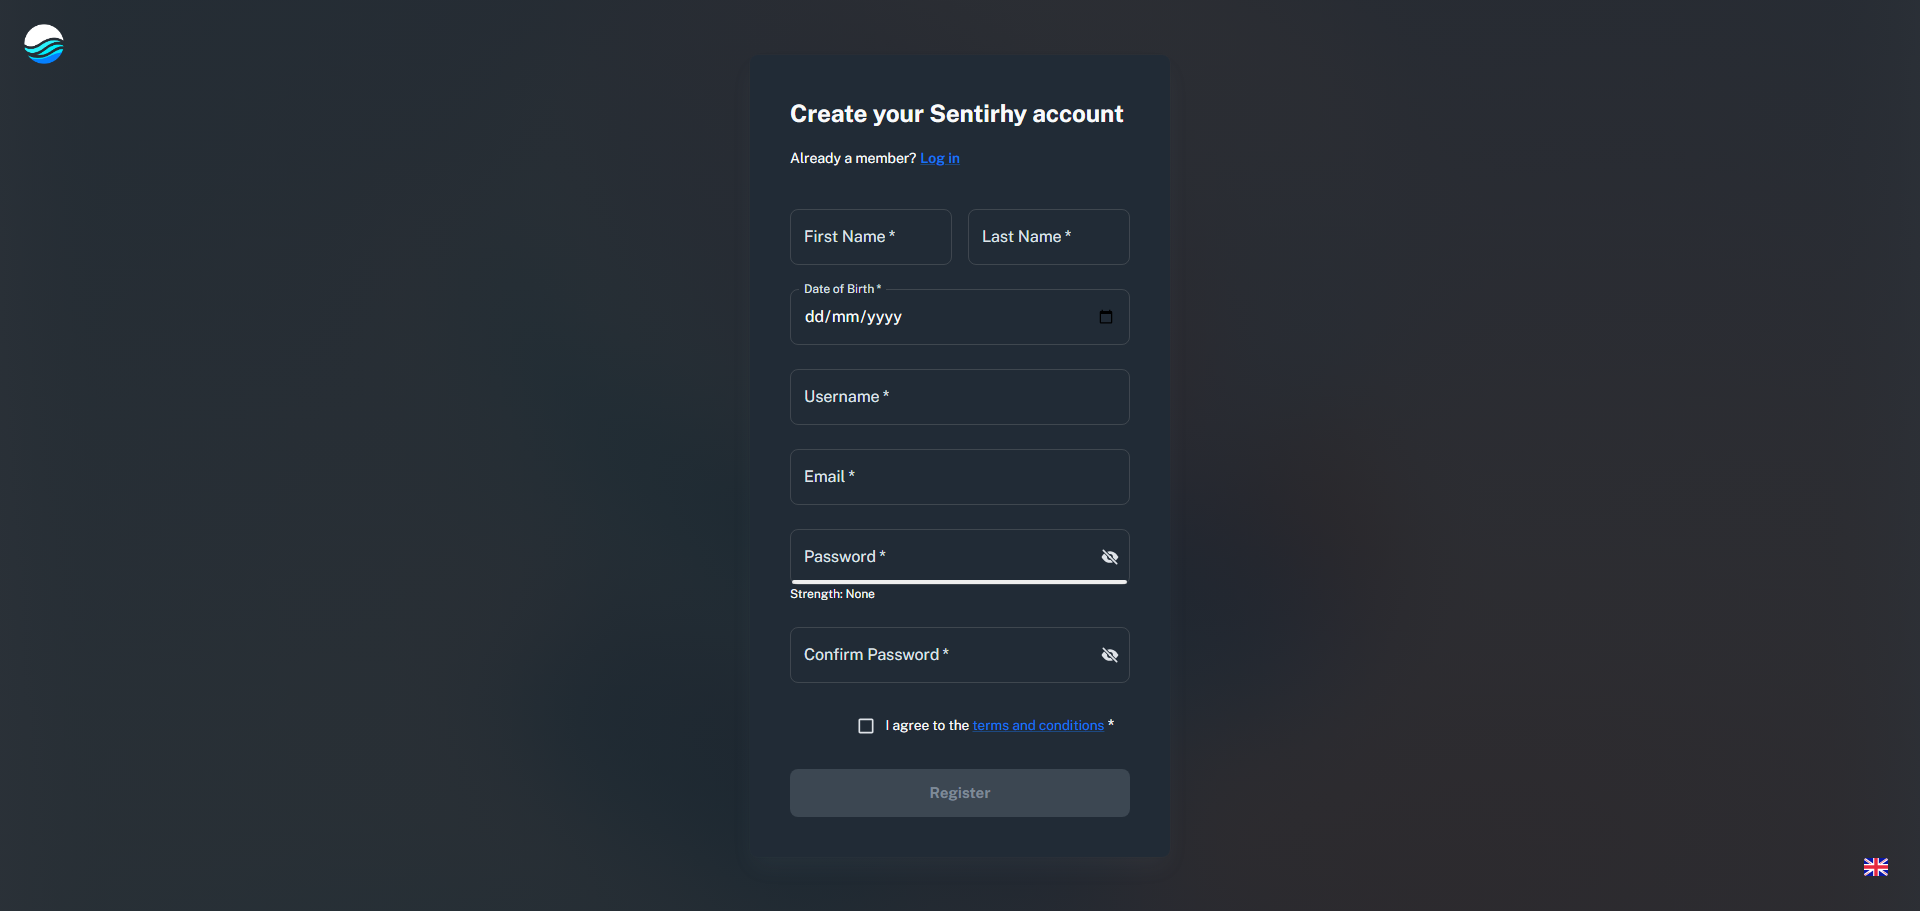
\includegraphics[width=14cm]{Images/register-ui.png}
    \caption{Register Page - UI}
    \label{fig:register-page-ui}
\end{figure}
Users first provide their personal information, which consists of their date of birth, fist and last names, preferred username, and email address, to begin the registration process. (Figure \ref{fig:register-page-ui}) 
The entered data is then validated by cross-referencing it with existing entries in the `sentirhy.user' table within the PostgreSQL database.
If there is duplicated username or email, the user will be notified that the credentials have already been taken and the process will stopped.
When there is no duplicate entry, the user's password is securely hashed with `bcrypt', and the crypto module sends an unique activation token to the user's email for account verification.
The generated token with an expiration date is also stored in the database with the user credentials for security purposes. 
\\
\begin{figure}[h!]
    \centering
    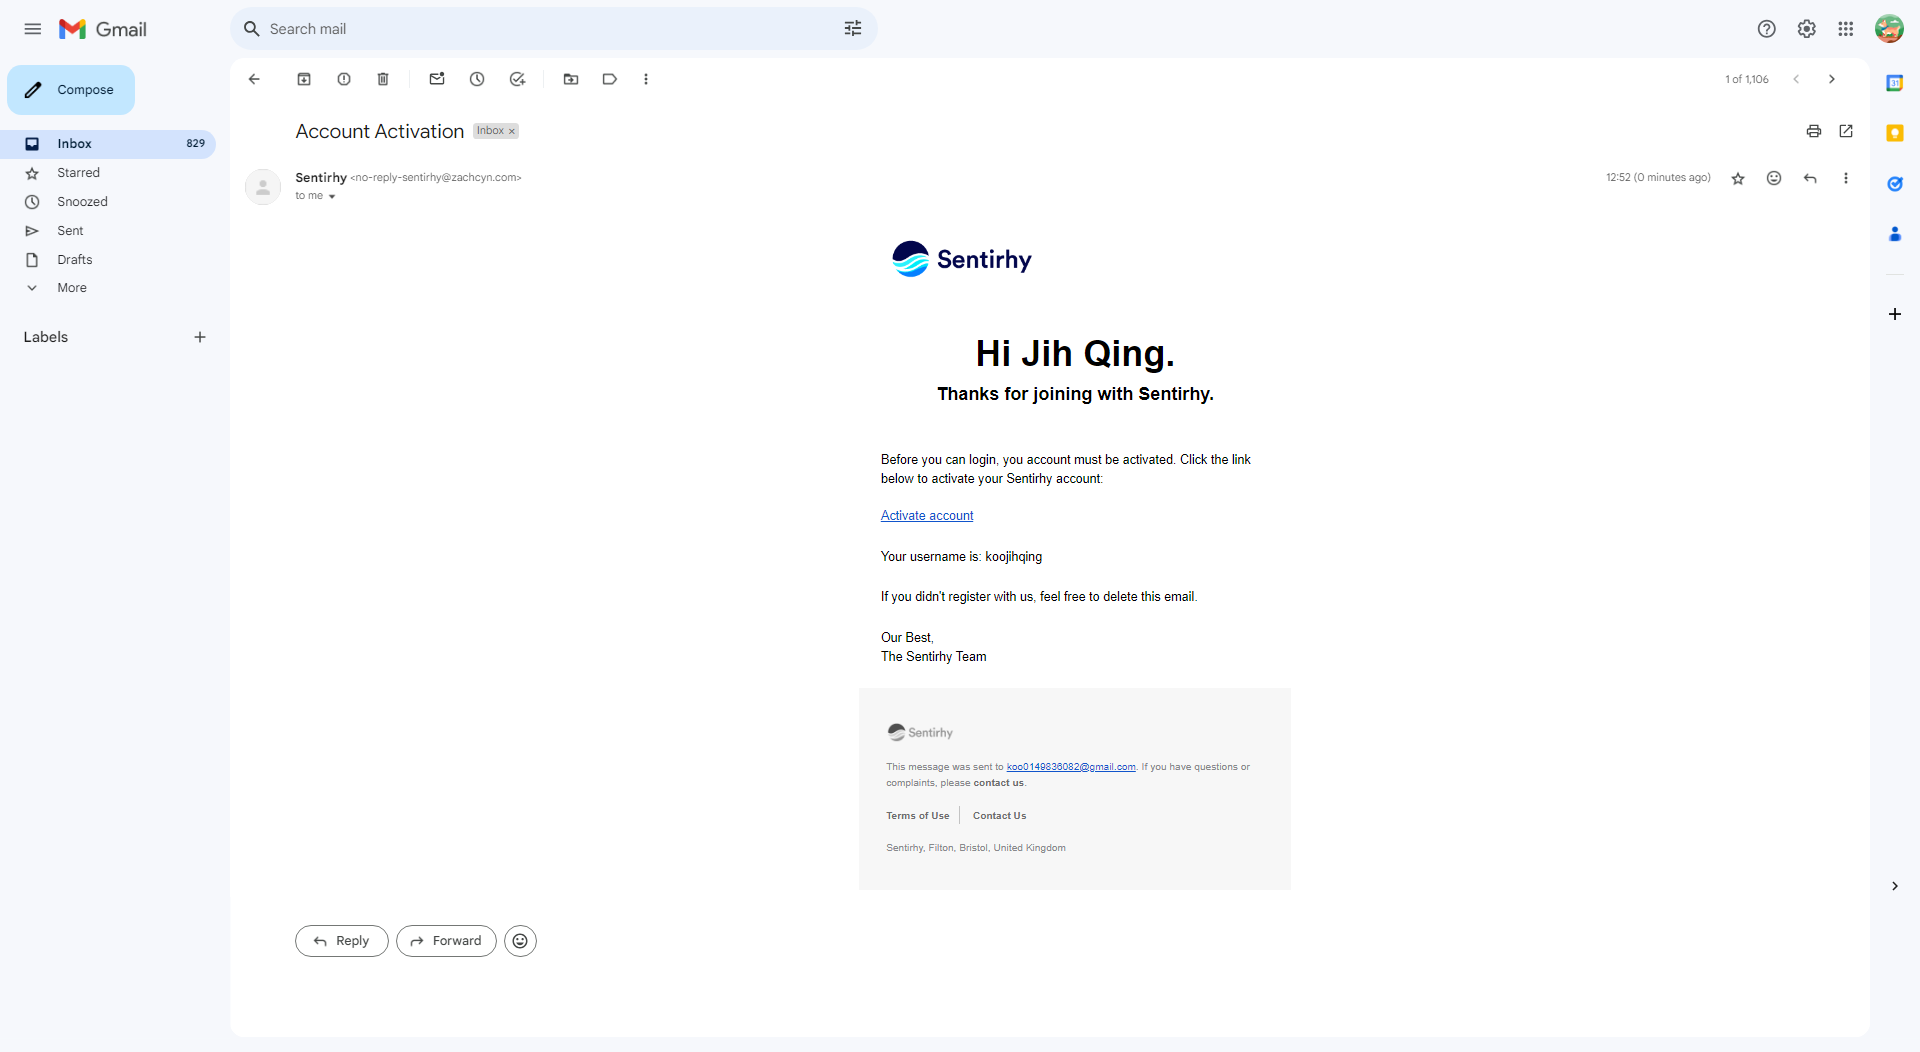
\includegraphics[width=14cm]{Images/acc-activation.png}
    \caption{Account Activation Email - UI}
    \label{fig:account-activation-ui}
\end{figure}
\begin{figure}[h!]
    \centering
    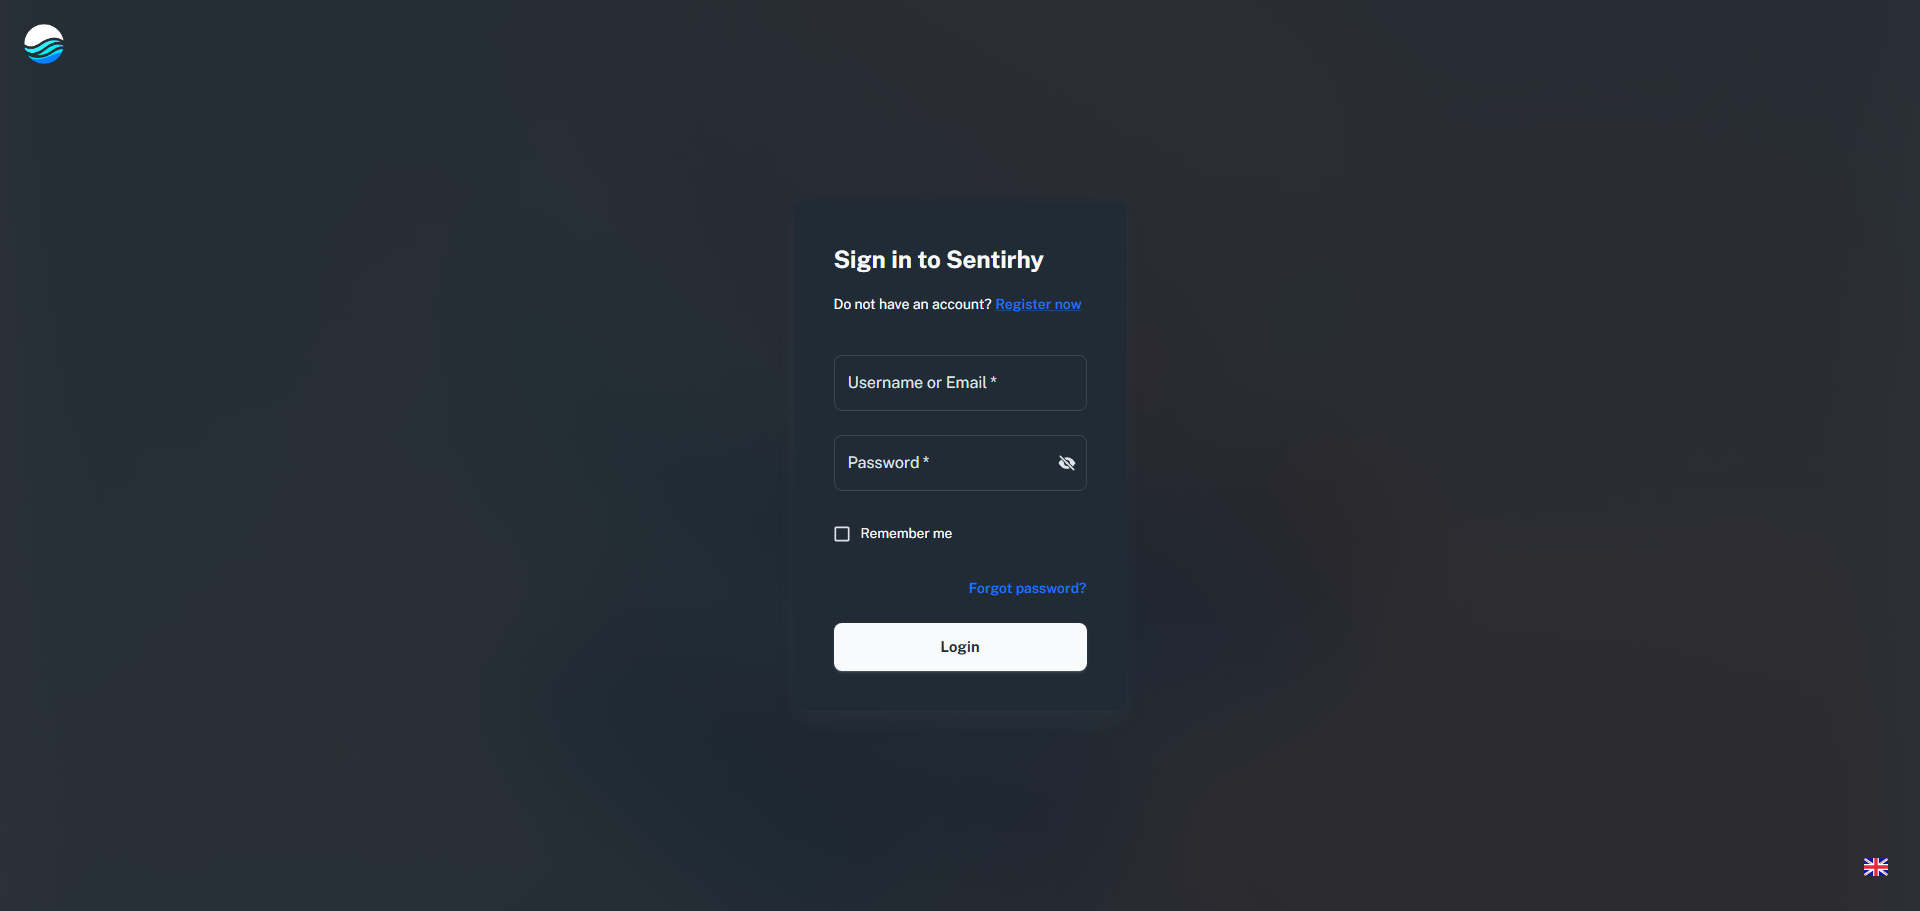
\includegraphics[width=14cm]{Images/login-ui.png}
    \caption{Login Page - UI}
    \label{fig:login-page-ui}
\end{figure}
\\
\indent An activation email (Figure \ref{fig:account-activation-ui}) is sent out using the `nodemailer' after the new user's database entry.
For the login process (Figure \ref{fig:login-page-ui}), the username and password are required.
After user submitted the credentials, the system compares those credentials to those kept in the database. 
Then, access to the application is granted with a successful match and an activated account.
\\
\subsection{Integration with Music Services}
\begin{figure}[h!]
    \centering
    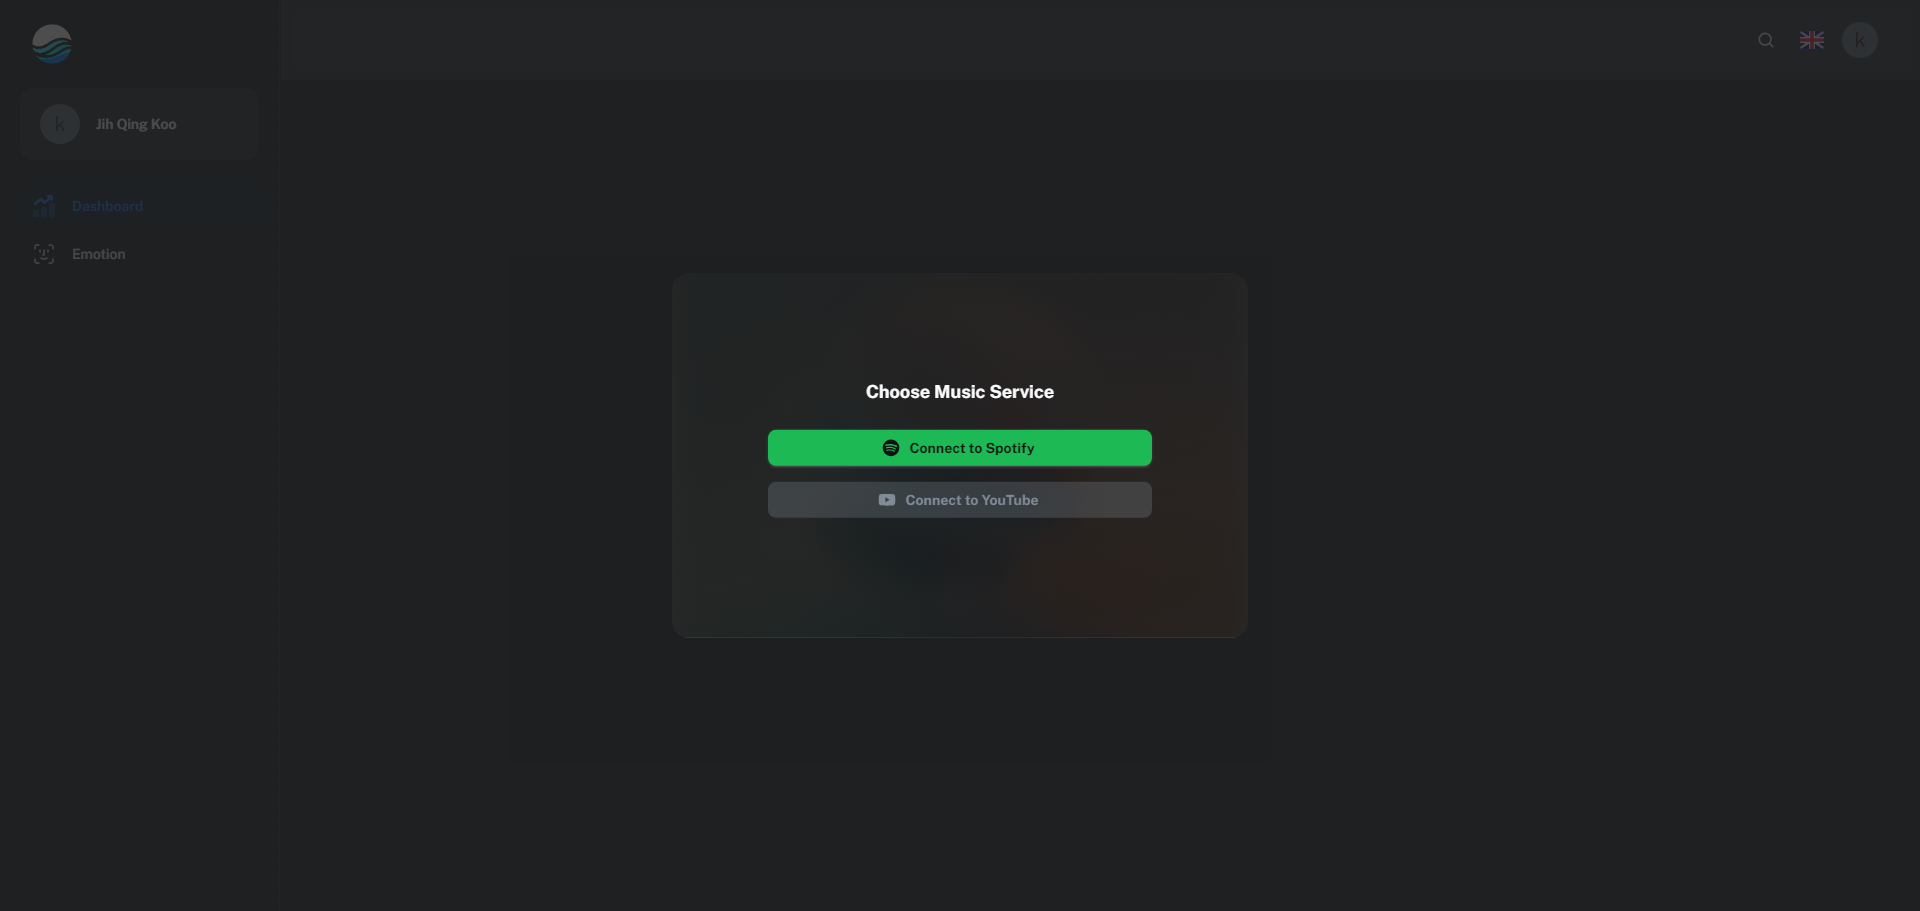
\includegraphics[width=14cm]{Images/connect-api.png}
    \caption{Music Services Connection - UI}
    \label{fig:music-service}
\end{figure}
As users log into the application, they are greeted with a dashboard.
There will be a modal component (Figure~\ref{fig:music-service}) showing on the dashboard, allowing users to connect to different music services, which is required to the app's function to play music.
Users are redirected to Spotify's authorization interface through an OAuth 2.0 authorization flow in order to grant permissions when they choose to link their accounts.
Once user's permission is acquired, an access token from Spotify's token endpoint gives the application the authority to request services from the Spotify API on the user's behalf, like playing music.
Unfortunately, as of right now, the only integration that is operational is Spotify; Youtube connectivity is indicated as a planned addition.
\\
\subsection{Emotion Detector}
\begin{figure}[h!]
    \centering
    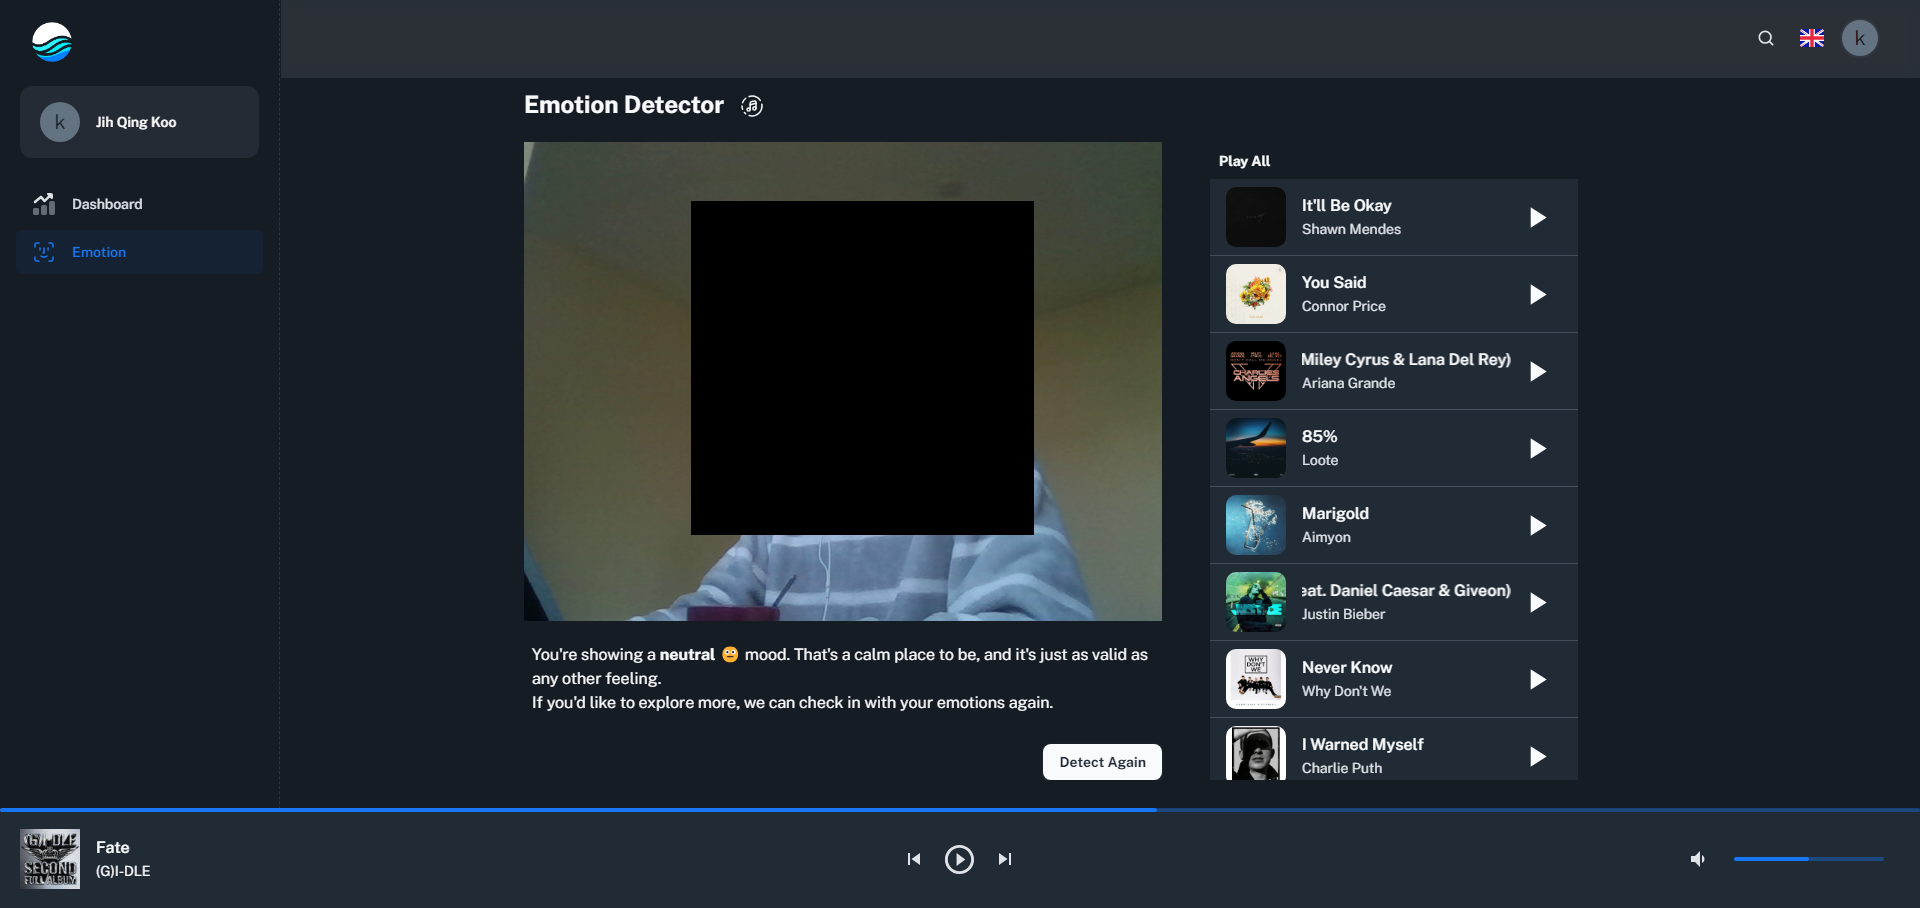
\includegraphics[width=14cm]{Images/emotion-detector.png}
    \caption{Emotion Detector - UI}
    \label{fig:emo-detect}
\end{figure}
When user enters the Emotion Detection page (Figure~\ref{fig:emo-detect}), they encounter an interactive interface that requires access to the camera to proceed.
With the user's permission, the application launches the Haarcascade frontal face identification algorithm and opencv.js, the \gls{js} library of OpenCV, enabling real-time face detection through the live video feed.
\\
\begin{figure}[h!] 
    \centering
\begin{minted}[frame=lines, framesep=2mm, baselinestretch=1.2, fontsize=\footnotesize, linenos, breaklines]{python}
    async function predictEmotion(imageFilename) {
        const imagePath = path.join(__dirname, '/user_emotion/', imageFilename);
        const model = await loadModel()
        const imageBuffer = await fs.promises.readFile(imagePath);
        const tensor = tf.node.decodeImage(imageBuffer).resizeBilinear([48, 48]).mean(2).expandDims(-1).expandDims(0).toFloat().div(tf.scalar(255));
        const prediction = model.predict(tensor);
        const emotionIndex = prediction.argMax(1).dataSync()[0];

        return emotions[emotionIndex];
    }
\end{minted}
    \caption{Load Model and Preprocess data}
    \label{fig:load-process}
\end{figure}
\indent The system is designed to identify faces quickly and captures the frame.
The captured frame is then sent to the backend in a binary format appropriate for transmission over the network.
The backend, which has been configured with TensorFlow.js, awaits the binary format data to perform its function.
It loads the trained model, then resize the image to 48x48 pixels, converted to grayscale, normalized to scale the pixel values, and batched for the model's evaluation in order to meet the model's needs. (Figure~\ref{fig:load-process})
\\
\begin{figure}[h!] 
    \centering
\begin{minted}[frame=lines, framesep=2mm, baselinestretch=1.2, fontsize=\footnotesize, linenos, breaklines]{python}
    function generateProgressivePlaylist(user_emotion_tracks, neutral_tracks, happy_tracks, playlistLength) {

        const allTracks = user_emotion_tracks.concat(neutral_tracks, happy_tracks);
        allTracks.sort((a, b) => a.valence - b.valence);
        const step = Math.floor(allTracks.length / playlistLength);

        const selectedTracks = [];
        for (let i = 0; i < playlistLength && (i * step) < allTracks.length; i++) {
            selectedTracks.push(allTracks[i * step]);
        }

        return selectedTracks;
    }
\end{minted}
    \caption{Generate Playlist}
    \label{fig:generate-playlist}
\end{figure}
\indent When the image is in an acceptable format, the model starts to recognize the user's current emotional state.
Once the emotion is deciphered, the system responds by creating playlist that corresponds with the feeling. (Figure~\ref{fig:generate-playlist})
The generated playlist is then dynamically displayed on the \gls{ui}.
 % Section/Chapter entries can be done in the Main.tex file or in a  
                       % separate tex file for longer and more complex documents

% -------------------  PROJECT EVALUATION  ---------------------
\chapter{Project Evaluation}
\section{Introduction}
Project evaluation allows to reflect on the project's successes and limitations.
The end product was a responsive web application combined with advanced machine learning algorithms to create an emotion-based music recommendation system.
\gls{cnns} model at the core of the system was trained on robust datasets and refined through transfer learning to improve recognition accuracy, especially for underrepresented demographics.
This section is an opportunity to consider the feedback loop form supervisor, integrating their thoughts into the project's development.

\subsection{Reflection on Project Phases}
To improve the project's foundation, the research phase needs to include a deeper look into several key areas.
First, integrating empirical research and well-established psychological theories will enrich the scientific basis of the emotion-music interaction, supporting the algorithmic approach for music recommendation.
Additionally, adaptive algorithms that can customize recommendations based on user feedback should also be considered to improve user engagement and satisfaction.
\\
\indent To ensure the system's global applicability and adherence to ethical standards, especially privacy and cultural sensitivity, it is also essential to address ethical and cultural issues.
Last but not least, by recognizing and addressing the limitations of current music therapy practices, the project may be positioned as a technical advancement that provides accessible and personalized therapeutic solutions.
\\
\indent The project was originally designed with a defined set of features that were essential for a music therapy application, such as user registration, emotion detection, music recommendations, along with an integration with Spotify's Web Playback API.
However, as the project developed, emerging challenges and deeper insights made it necessary to reevaluate and modify these requirements.
As the appendix's Gantt chart (Figure~\ref{fig:gantt-chart}) shows, the development of \gls{ml} models and the integration with Spotify's API took longer than expected. 
The main cause of these delays was the unfamiliar with integrating API into web application and discovering the way to enhance the model's performance but still considering the amount of computational resources required.
\\
\indent Due to the delay which cause time constraints, the YouTube API integration was deprioritized and eventually not deployed.
This decision is made to ensure the project could proceed gradually and the robustness and functionality of the core features, which were critical to the project's success, are developed on time.
\\
\indent During the implementation phase, a well-chosen technology stack and adaptable development techniques helped the project to be completed.
The PERN stack was chosen for its reliability and scalability. 
The agile methodologies was chosen as it allows iterative improvements and flexibility in response to changing project requirements.
\\
\indent Using opencv.js for real-time face identification in the web application was one of the biggest obstacles, which required significant technical adjustments to ensure compatibility and efficiency.
Another considerable challenge was the intensive hyperparameter tuning required for the models, especially the second one, for which it took approximately seven days to go through the parameter grid (Figure~\ref{fig:param_grid}). 
Then, the project timeline was impacted by this procedure, which was important but time-consuming.

\subsection{Limitations and Test Results}
In project evaluation, it is critical to address the limitations.
One significant limitation in the emotion recognition system was its varying accuracy when exposed to different lighting conditions or when faced with unusual facial expressions, which may affect the accuracy of the results.
\\
\indent Additionally, even though the models work excellent on the dataset used, there were limits to the datasets themselves.
For example, there were diversity issues with the datasets, FER2013 (Figure~\ref{fig:fer2013}) and CK+ (Figure~\ref{fig:ckextended}), especially with regard to ethnic representation.
Also, the model may become biased towards to those more commonly represented categories, such as `Neutral' faces in FER2013.
This could limits the system applicability in real-world and diverse settings.
\\
\indent As Table \ref{tab:test-case} showed, the project went through a set of testing that covered a wide range of functionality from backend operations to user interface interactions.
The test showed the application's capability to handle user interactions and to interface with other services in an effective way. 
Tests for \gls{fer} validated the face recognition algorithms' reliability, which is crucial for the project's core functionality.
But, scalability testing, which is essential for evaluating the application's performance under various load conditions, is not part of the testing. 

\subsection{Supervisor's Feedback Utilization}
The scope of the project was refined due to the frequent communication with the supervisor (Table~\ref{tab:meeting-log}). 
The project was previously intended to identify seven different emotions: angry, sad, neutral, happy, disgust, fear, and surprise.
However, based on observations highlighting the importance of these fundamental emotions in music therapy, the scope was reduced to just focus on the first four.
This modification ensured that the system was built with a clear focus on usability and efficacy for real-world applications, which also reduced the complexity and brought the project more directly in line with its therapeutic aims.
 % Section/Chapter entries can be done in the Main.tex file or in a  
                       % separate tex file for longer and more complex documents
                                           
% -------------------  BIBLIOGRAPHY ---------------------
\newpage
% \bibliographystyle{abbrvnat}
\bibliographystyle{agsm}
\bibliography{References}
\addcontentsline{toc}{chapter}{References} % Adds References Section to Table of Contents
% -------------------  Appendix  ---------------------
\chapter*{Appendix}
\addcontentsline{toc}{chapter}{Appendix}
% Appendix A

% \addcontentsline{toc}{section}{Appendix A}
\section{}
\label{app:appendix-a}

\begin{minted}[frame=single, framesep=2mm, baselinestretch=1.2, fontsize=\footnotesize, breaklines,linenos, numbersep=5pt]{text}
2023-12-27 23:22:26.546868:
(32, 64, 128, 128, 3, 3, 3, 3, 0.1, 0.0, 0.0, 512, 'adam', 32, 10) CHECKED
Best Score: 0.5725693106651306
Best Params: {'conv_1_filters': 32, 'conv_2_filters': 64, 'conv_3_filters': 128, 'conv_4_filters': 128, 'conv_1_kernel': 3, 'conv_2_kernel': 3, 'conv_3_kernel': 3, 'conv_4_kernel': 3, 'dropout_1': 0.1, 'dropout_2': 0.0, 'dropout_3': 0.0, 'dense_units': 512, 'optimizer': 'adam'}
(32, 64, 128, 128, 3, 3, 3, 3, 0.1, 0.0, 0.0, 768, 'adam', 32, 10) CHECKED
Best Score: 0.5725693106651306
Best Params: {'conv_1_filters': 32, 'conv_2_filters': 64, 'conv_3_filters': 128, 'conv_4_filters': 128, 'conv_1_kernel': 3, 'conv_2_kernel': 3, 'conv_3_kernel': 3, 'conv_4_kernel': 3, 'dropout_1': 0.1, 'dropout_2': 0.0, 'dropout_3': 0.0, 'dense_units': 512, 'optimizer': 'adam'}
2023-12-27 23:24:26.831029:
(32, 64, 128, 128, 3, 3, 3, 3, 0.1, 0.0, 0.0, 1024, 'adam', 32, 10) CHECKED
Best Score: 0.5765619874000549
Best Params: {'conv_1_filters': 32, 'conv_2_filters': 64, 'conv_3_filters': 128, 'conv_4_filters': 128, 'conv_1_kernel': 3, 'conv_2_kernel': 3, 'conv_3_kernel': 3, 'conv_4_kernel': 3, 'dropout_1': 0.1, 'dropout_2': 0.0, 'dropout_3': 0.0, 'dense_units': 1024, 'optimizer': 'adam'}
2023-12-27 23:25:37.281540:
(32, 64, 128, 128, 3, 3, 3, 3, 0.1, 0.0, 0.2, 512, 'adam', 32, 10) CHECKED
Best Score: 0.5906981825828552
Best Params: {'conv_1_filters': 32, 'conv_2_filters': 64, 'conv_3_filters': 128, 'conv_4_filters': 128, 'conv_1_kernel': 3, 'conv_2_kernel': 3, 'conv_3_kernel': 3, 'conv_4_kernel': 3, 'dropout_1': 0.1, 'dropout_2': 0.0, 'dropout_3': 0.2, 'dense_units': 512, 'optimizer': 'adam'}
2023-12-27 23:26:47.249360: 
(32, 64, 128, 128, 3, 3, 3, 3, 0.1, 0.0, 0.2, 768, 'adam', 32, 10) CHECKED
Best Score: 0.5906981825828552
Best Params: {'conv_1_filters': 32, 'conv_2_filters': 64, 'conv_3_filters': 128, 'conv_4_filters': 128, 'conv_1_kernel': 3, 'conv_2_kernel': 3, 'conv_3_kernel': 3, 'conv_4_kernel': 3, 'dropout_1': 0.1, 'dropout_2': 0.0, 'dropout_3': 0.2, 'dense_units': 512, 'optimizer': 'adam'}
2023-12-27 23:27:57.635618: 
(32, 64, 128, 128, 3, 3, 3, 3, 0.1, 0.0, 0.2, 1024, 'adam', 32, 10) CHECKED
Best Score: 0.5906981825828552
Best Params: {'conv_1_filters': 32, 'conv_2_filters': 64, 'conv_3_filters': 128, 'conv_4_filters': 128, 'conv_1_kernel': 3, 'conv_2_kernel': 3, 'conv_3_kernel': 3, 'conv_4_kernel': 3, 'dropout_1': 0.1, 'dropout_2': 0.0, 'dropout_3': 0.2, 'dense_units': 512, 'optimizer': 'adam'}
2023-12-27 23:29:09.047680:
(32, 64, 128, 128, 3, 3, 3, 3, 0.1, 0.0, 0.3, 512, 'adam', 32, 10) CHECKED
Best Score: 0.5906981825828552
Best Params: {'conv_1_filters': 32, 'conv_2_filters': 64, 'conv_3_filters': 128, 'conv_4_filters': 128, 'conv_1_kernel': 3, 'conv_2_kernel': 3, 'conv_3_kernel': 3, 'conv_4_kernel': 3, 'dropout_1': 0.1, 'dropout_2': 0.0, 'dropout_3': 0.2, 'dense_units': 512, 'optimizer': 'adam'}
2023-12-27 23:30:18.471026:
(32, 64, 128, 128, 3, 3, 3, 3, 0.1, 0.0, 0.3, 768, 'adam', 32, 10) CHECKED
Best Score: 0.5906981825828552
Best Params: {'conv_1_filters': 32, 'conv_2_filters': 64, 'conv_3_filters': 128, 'conv_4_filters': 128, 'conv_1_kernel': 3, 'conv_2_kernel': 3, 'conv_3_kernel': 3, 'conv_4_kernel': 3, 'dropout_1': 0.1, 'dropout_2': 0.0, 'dropout_3': 0.2, 'dense_units': 512, 'optimizer': 'adam'}
\end{minted}

\newpage

% \addcontentsline{toc}{section}{Appendix B}
\section{}
\label{app:appendix-b}

\newpage
\begin{landscape}
\section{}
\label{app:appendix-c}
\begin{longtable}{ |m{1cm}|m{1cm}|m{5cm}|m{5cm}|m{5cm}|m{2cm}| }
    \hline
    \rowcolor{lightgray}
    \textbf{Test No.} & \textbf{Cats.} & \textbf{Intention} & \textbf{Expected Result} & \textbf{Actual Result} & \textbf{Pass/Fail} \\
    \hline
    \endfirsthead

    \hline
    \rowcolor{lightgray}
    \textbf{Test No.} & \textbf{Cats.} & \textbf{Intention} & \textbf{Expected Result} & \textbf{Actual Result} & \textbf{Pass/Fail} \\
    \hline
    \endhead
    1 & \gls{ui} & Registration & User registered & User registered and information added to database & Pass \\
    \hline
    2 & \gls{ui} & Login & User logged in & User logged in successfully & Pass \\
    \hline
    3 & \gls{ui} & Incorrect credentials upon login & User login failed and error message display & Error message displayed and user unable to login & Pass \\
    \hline
    4 & \gls{ui} & Account Activation & User received email and activate account from link & User activate account successfully from link & Pass \\
    \hline
    \caption{Test Table}
\end{longtable}
\end{landscape}
 % Section/Chapter entries can be done in the Main.tex file or in a  
                       % separate tex file for longer and more complex documents                       

\end{document}
%  -------------------------------------------------
%  --------- The document ends from here ----------- 
%  -------------------------------------------------